%**************************************************************************************
% License:
% CC BY-NC-SA 4.0 (http://creativecommons.org/licenses/by-nc-sa/4.0/)
%**************************************************************************************

\documentclass[notes]{beamer}

\mode<presentation> {

\usetheme{Madrid}

% Burnt orange
\definecolor{burntorange}{rgb}{0.8, 0.33, 0.0}
\colorlet{beamer@blendedblue}{burntorange}
% Pale yellow
\definecolor{paleyellow}{rgb}{1.0, 1.0, 0.953}
\setbeamercolor{background canvas}{bg=paleyellow}
% Secondary and tertiary palett
\setbeamercolor*{palette secondary}{use=structure,fg=white,bg=burntorange!80!black}
\setbeamercolor*{palette tertiary}{use=structure,fg=white,bg=burntorange!60!black}

% To remove the footer line in all slides uncomment this line
%\setbeamertemplate{footline}
% To replace the footer line in all slides with a simple slide count uncomment this line
%\setbeamertemplate{footline}[page number]

% To remove the navigation symbols from the bottom of all slides uncomment this line
%\setbeamertemplate{navigation symbols}{}
}

\usepackage{amsmath}
\usepackage{bm}
\usepackage{breqn}
\usepackage{graphicx} % for figures
\usepackage{subcaption} % for subplots 
\usepackage[labelsep=space,tableposition=top]{caption}
\renewcommand{\figurename}{Fig.} 
\usepackage{cleveref}
\usepackage{caption,subcaption}% http://ctan.org/pkg/{caption,subcaption}
\usepackage{booktabs} % Allows the use of \toprule, \midrule and \bottomrule in tables
\usepackage{multirow}

% To print 2 slides on a page
%\usepackage{handoutWithNotes}
%\pgfpagesuselayout{2 on 1}[border shrink=2mm]
%----------------------------------------------------------------------------------------
%	TITLE PAGE
%----------------------------------------------------------------------------------------
% The short title appears at the bottom of every slide, the full title is only on the title page
\title[CE394M: FEM Geo]{CE394M: Finite Element Analysis in Geotechnical Engineering} 
\author{Krishna Kumar} % name
\institute[UT Austin] % institution 
{
University of Texas at Austin \\
\medskip
\textit{
  \url{krishnak@utexas.edu}} % Your email address
}
\date{\today} % Date, can be changed to a custom date

\begin{document}

\begin{frame}
\titlepage % title page as the first slide
\end{frame}

\begin{frame}
 % Table of contents slide, comment this block out to remove it
 \frametitle{Overview}
  %Throughout your presentation, if you choose to use \section{} and \subsection{} 
  %commands, these %will automatically be printed on this slide as an overview 
 \tableofcontents
\end{frame}

%----------------------------------------------------------------------------------------
% slides
%----------------------------------------------------------------------------------------
\section{Geotechnical FEA}
%------------------------------------------------
\begin{frame}
\frametitle{FE Disclaimer}
\begin{figure}[ht]
	\centering
	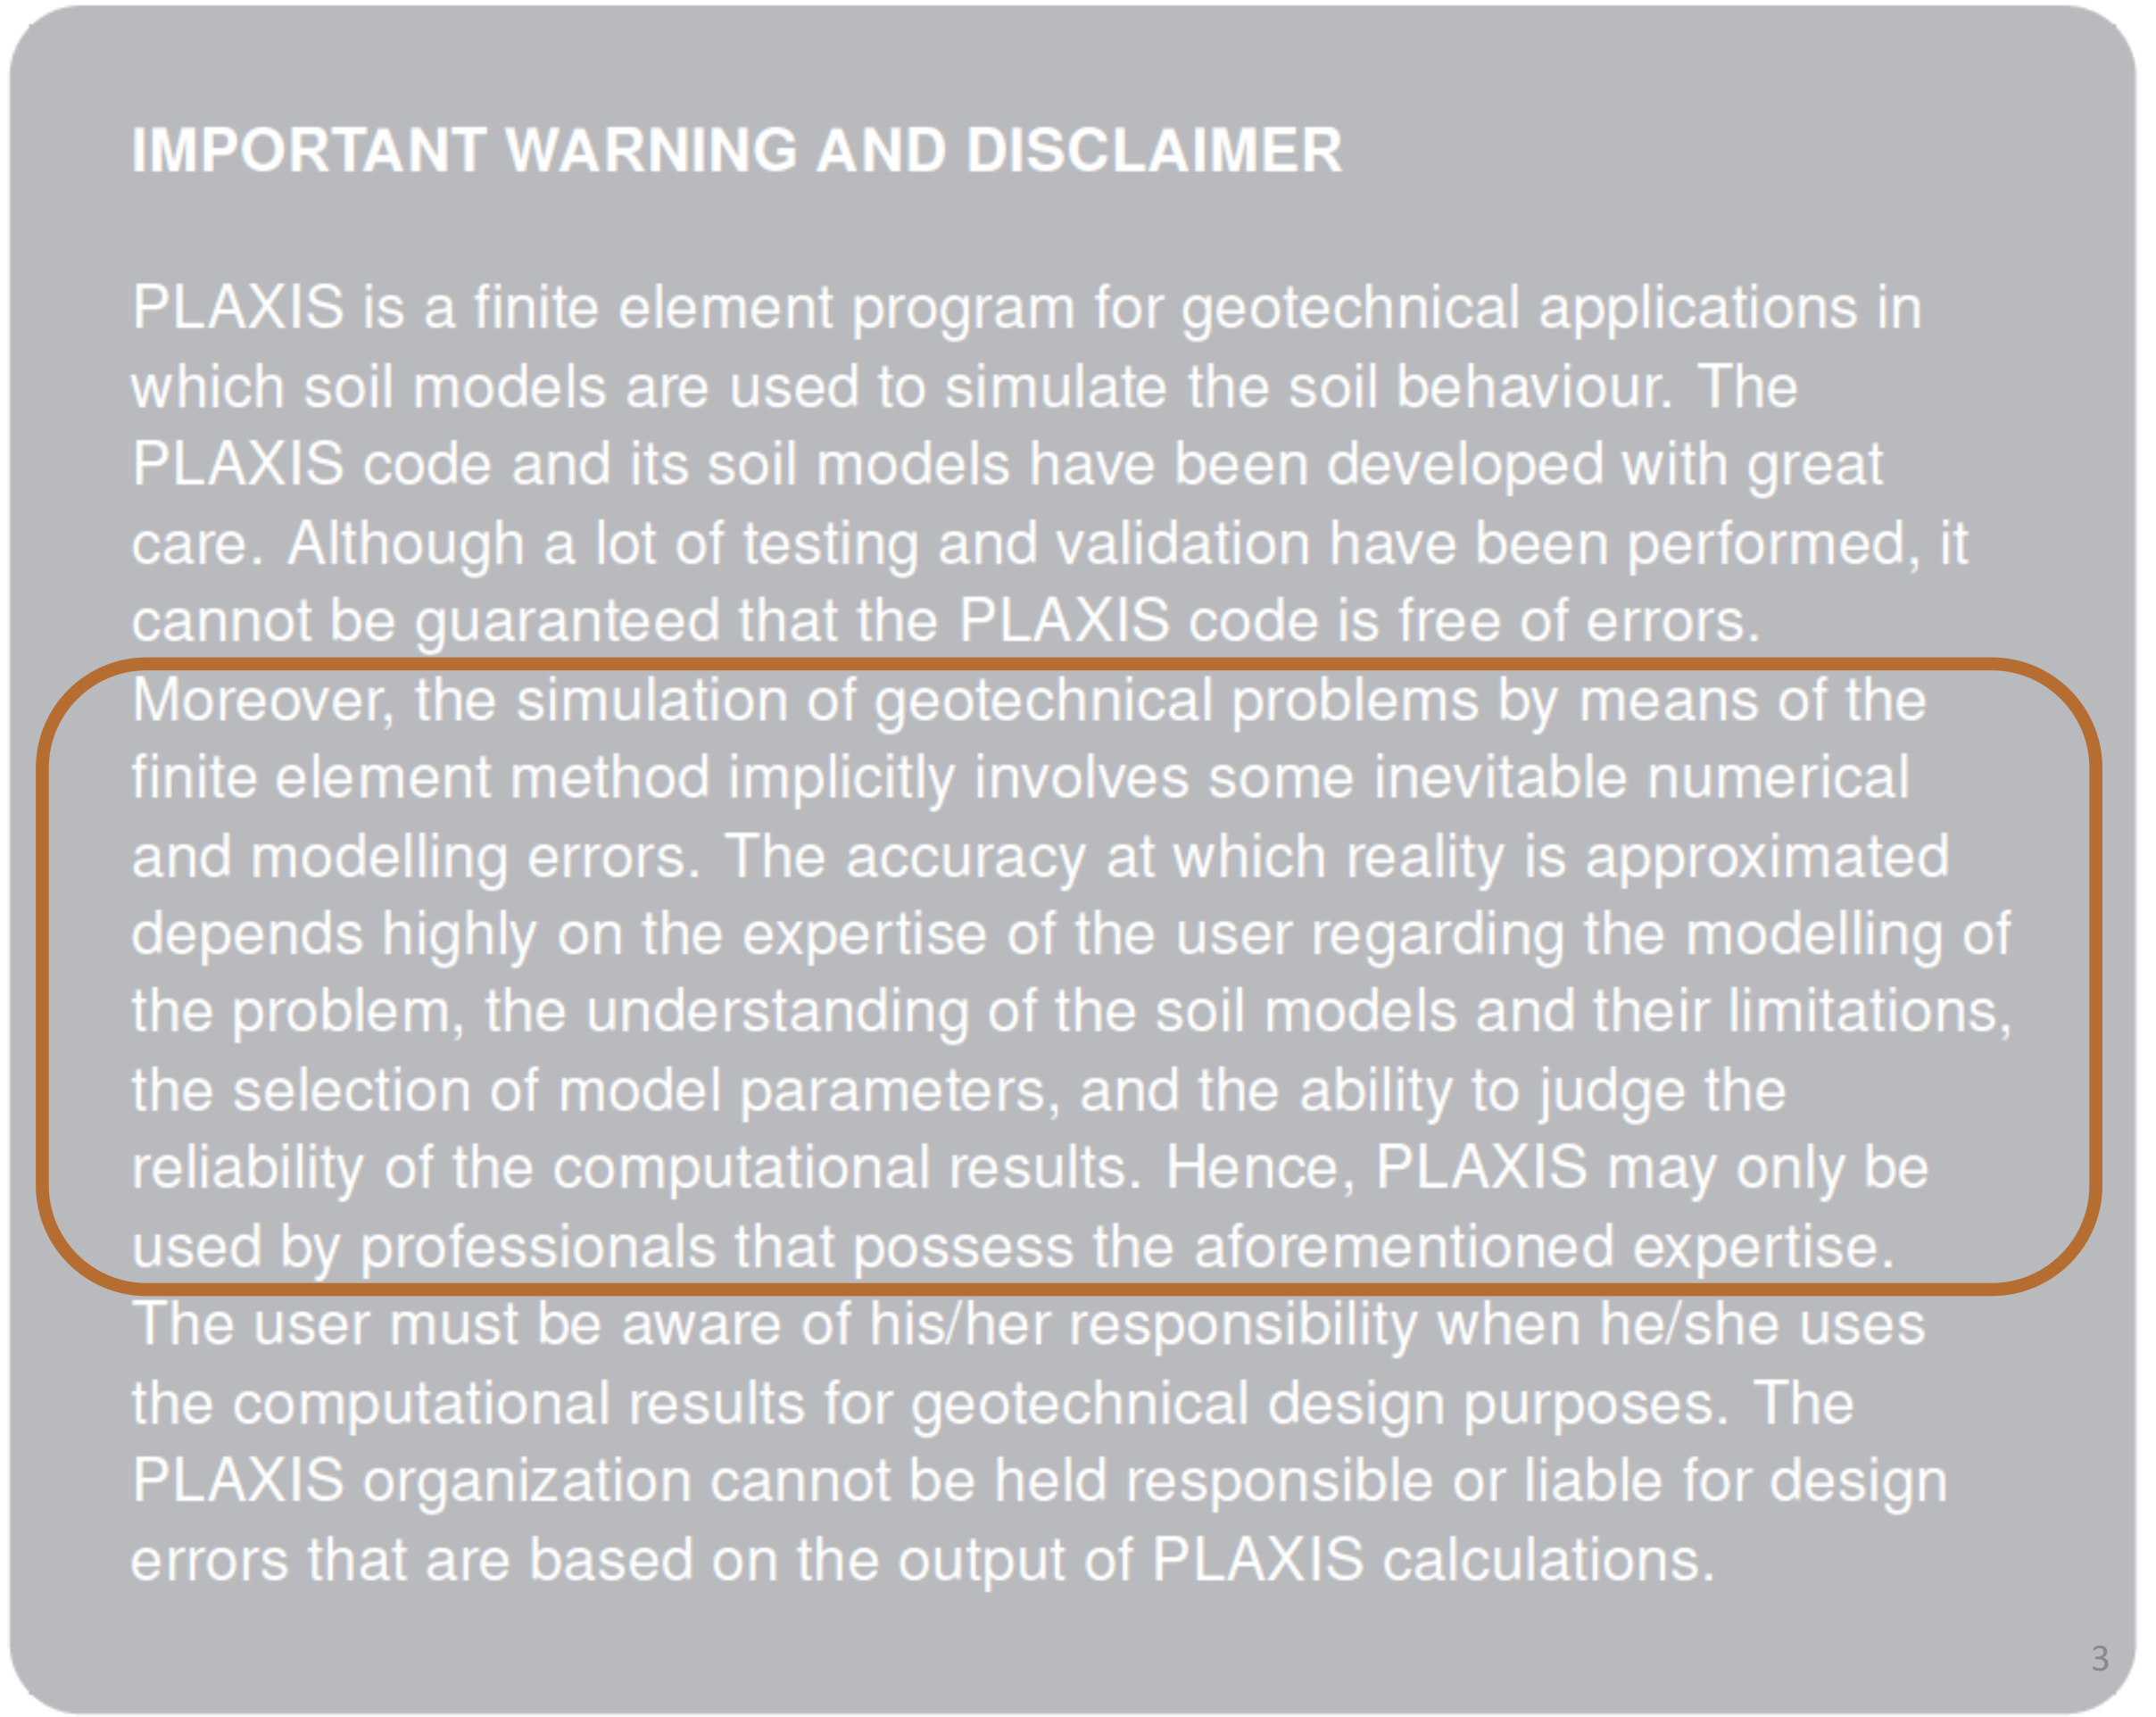
\includegraphics[width=0.85\textwidth]{figs/plaxis-disclaimer.png}
\end{figure}
\end{frame}

%------------------------------------------------
\begin{frame}
\frametitle{Consistent system of units}
\begin{figure}[ht]
	\centering
	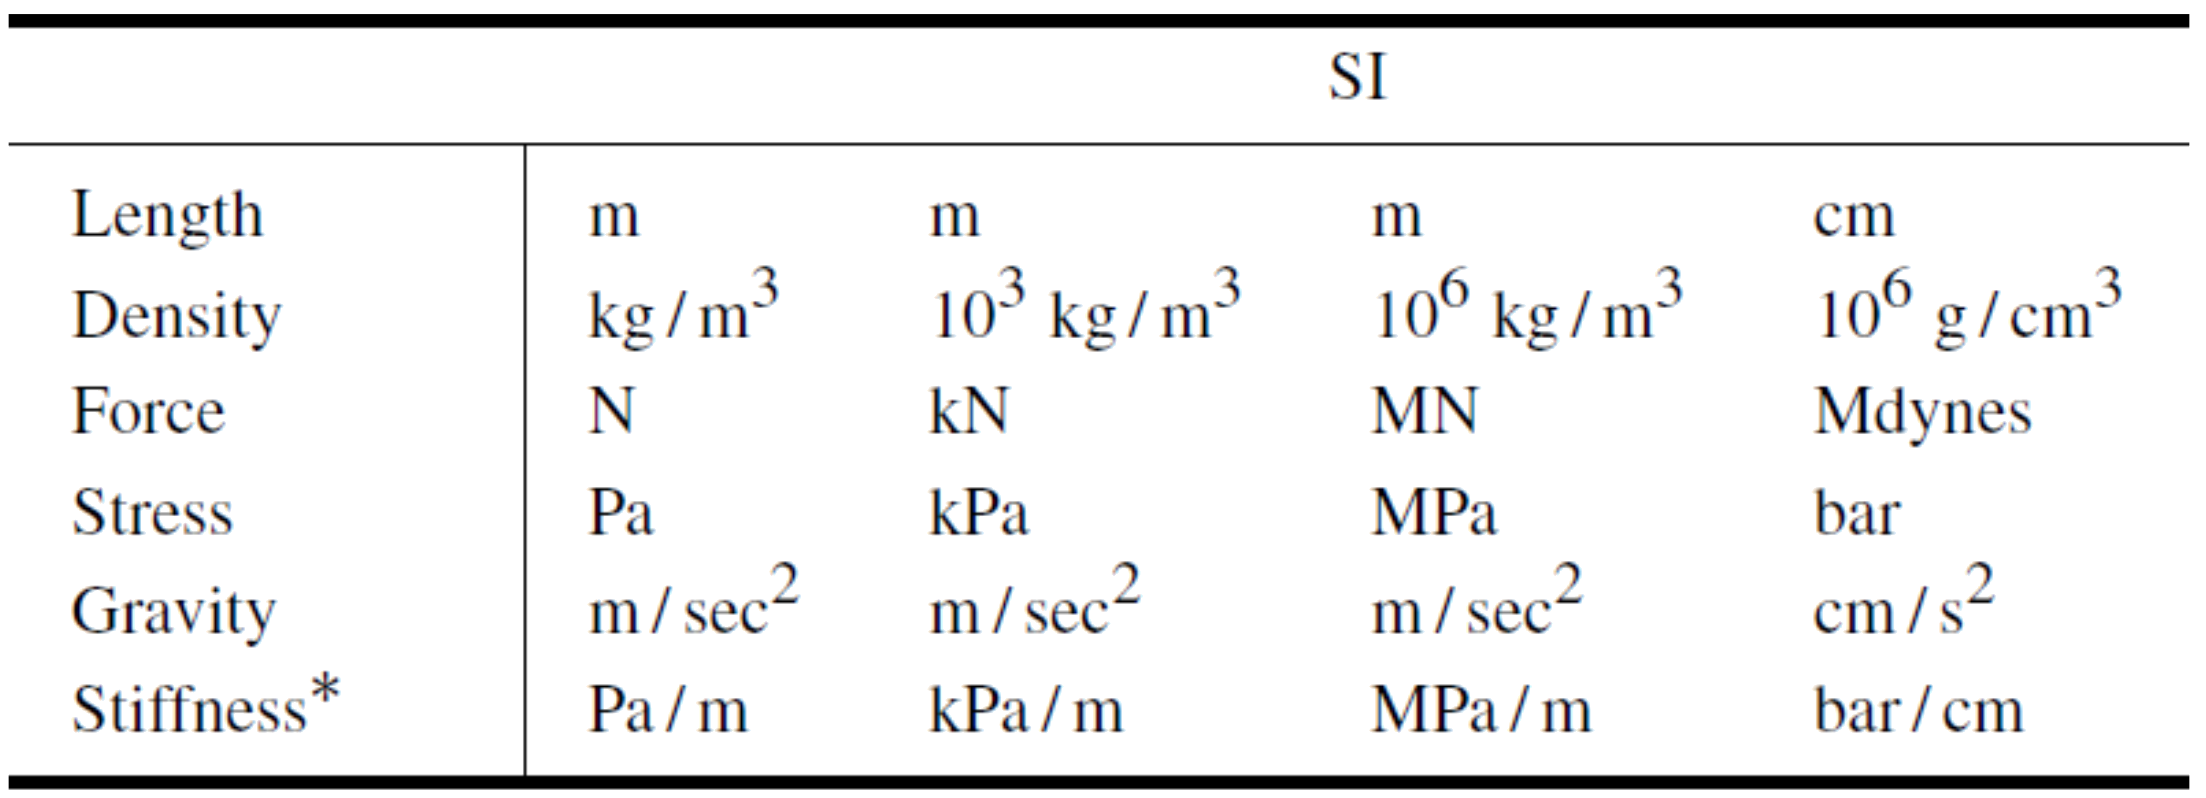
\includegraphics[width=0.85\textwidth]{figs/units.png}
\end{figure}
\end{frame}

%------------------------------------------------
\begin{frame}
\frametitle{Problem definition}
\mode<beamer>{
	\begin{figure}[ht]
		\centering
		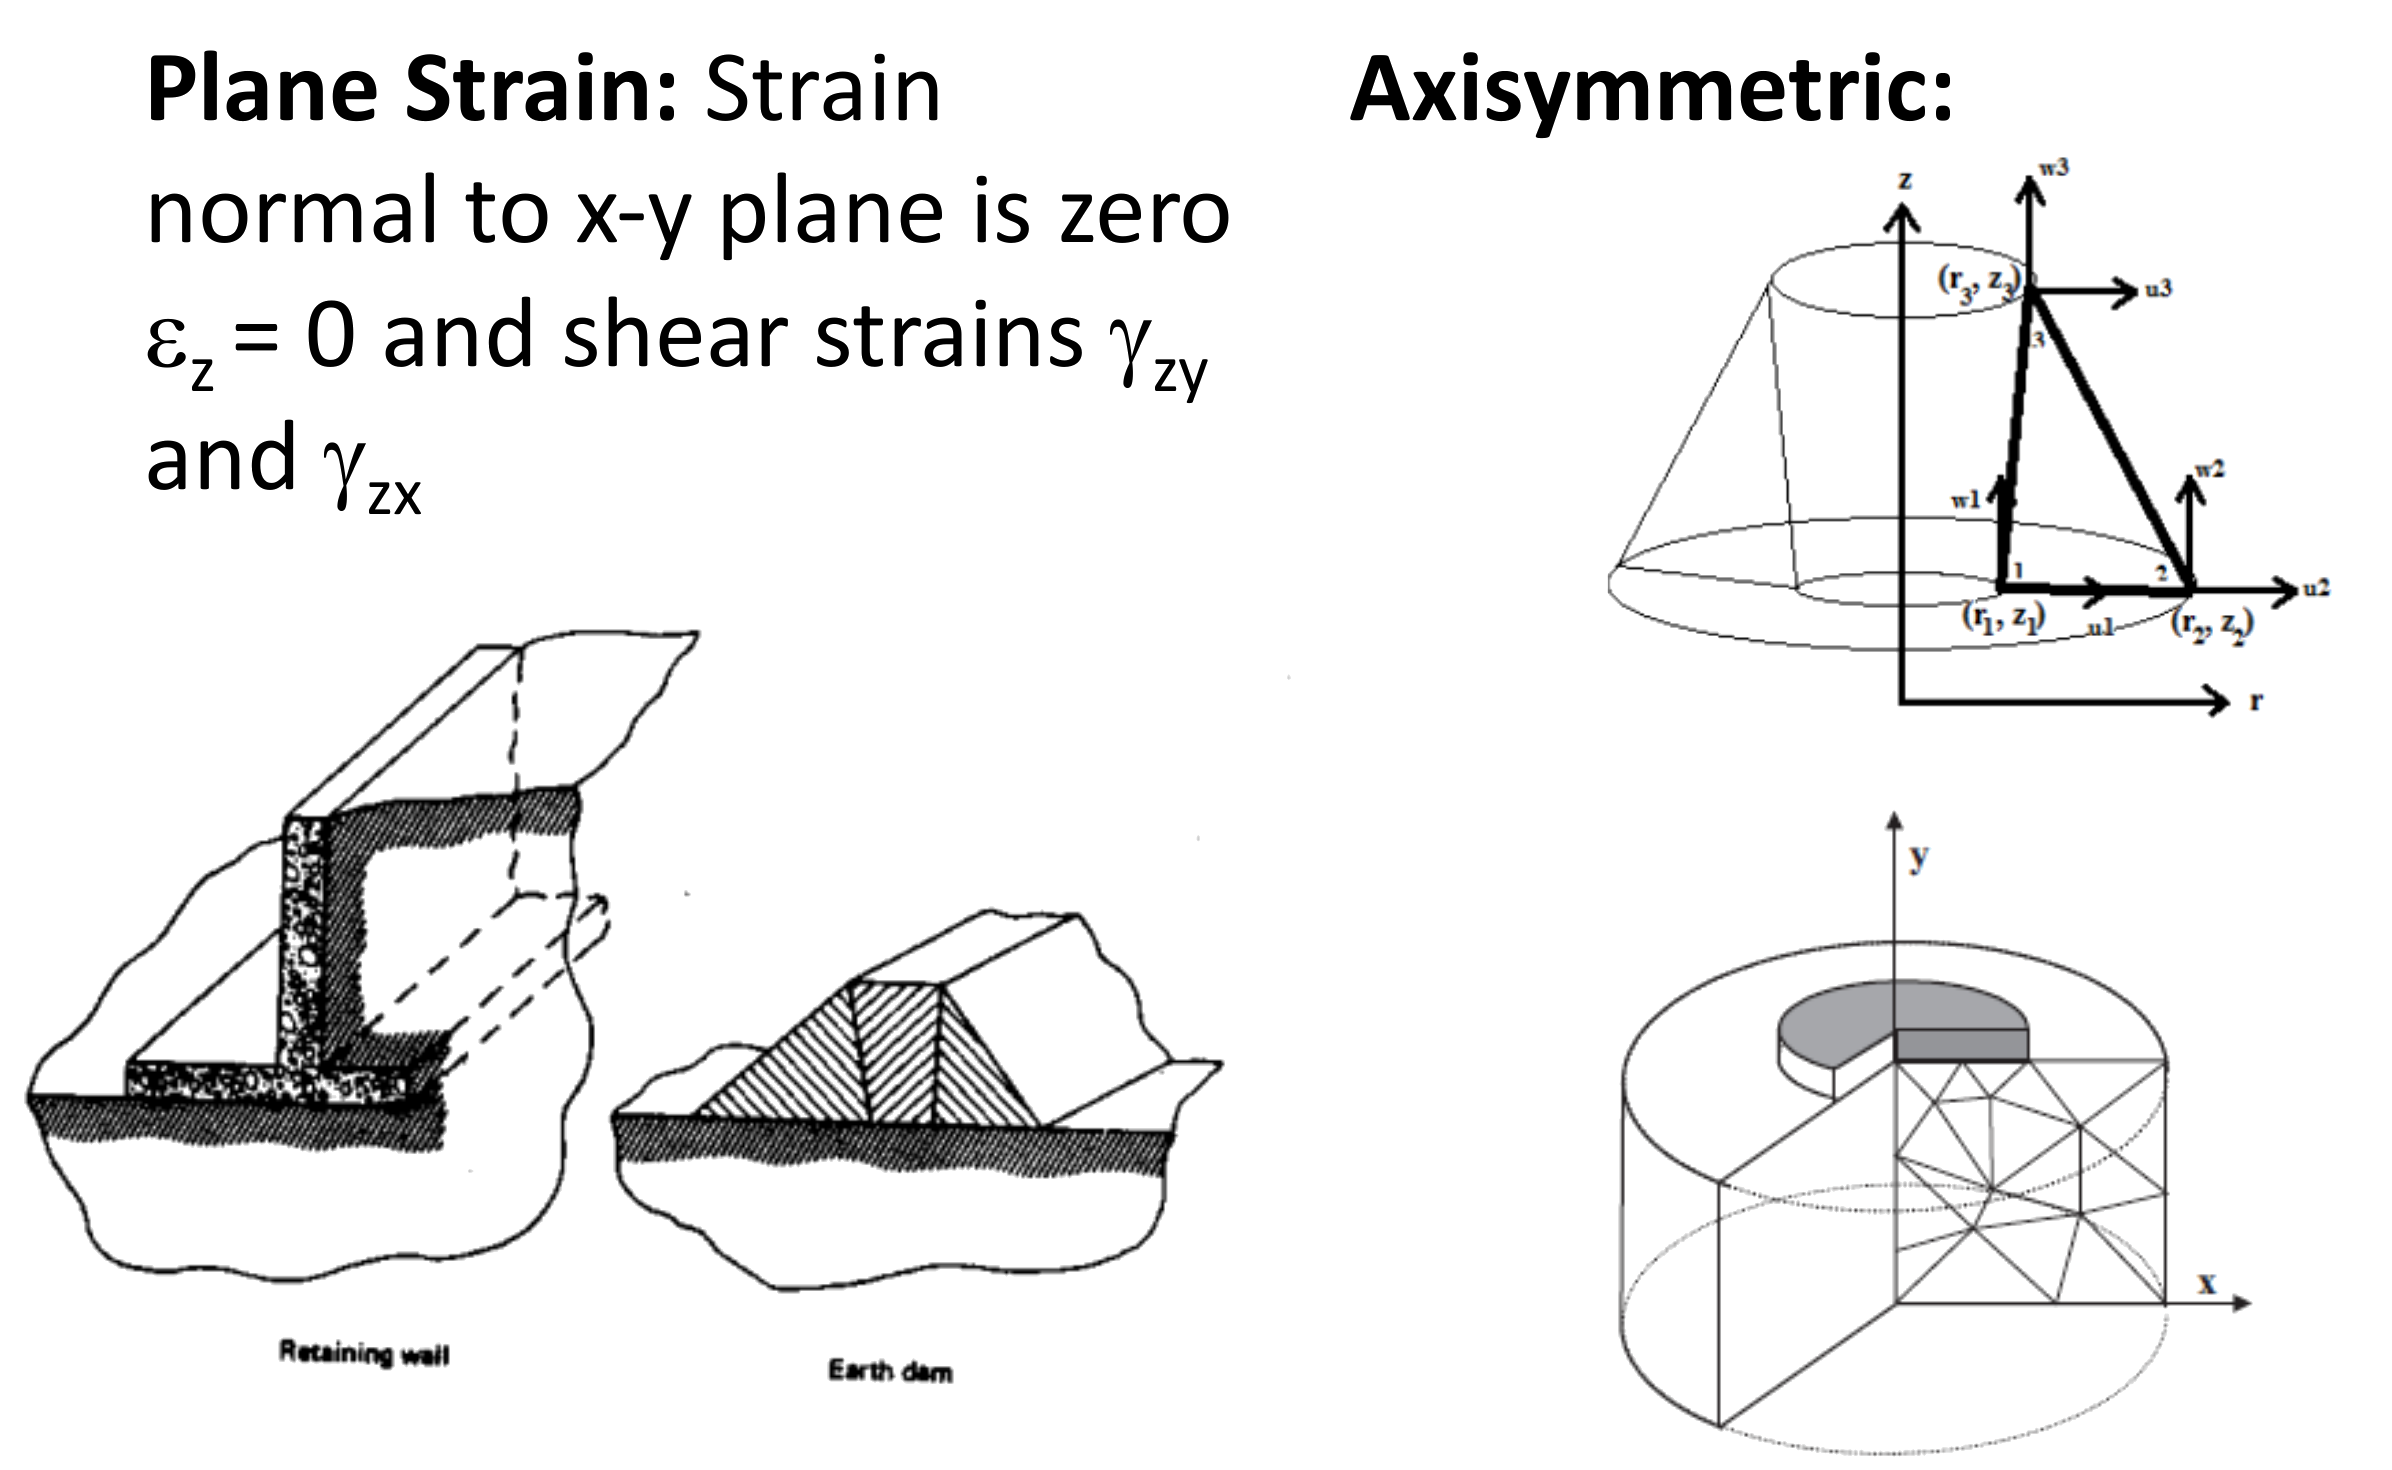
\includegraphics[width=0.85\textwidth]{figs/planestrain-axisymmetric.png}
		\caption*{Take advantage of symmetry}
	\end{figure}
}
\mode<handout>{
	\vspace{6cm}
}
\end{frame}

\subsection{Element types}
%------------------------------------------------
\begin{frame}
\frametitle{1D Finite Elements: Bar element}
Two node element with axial stiffness only (no flexural or shear
resistance).\mode<beamer>{Examples of this type of structure are cables, reinforcing bars.}
\begin{figure}[ht]
	\centering
	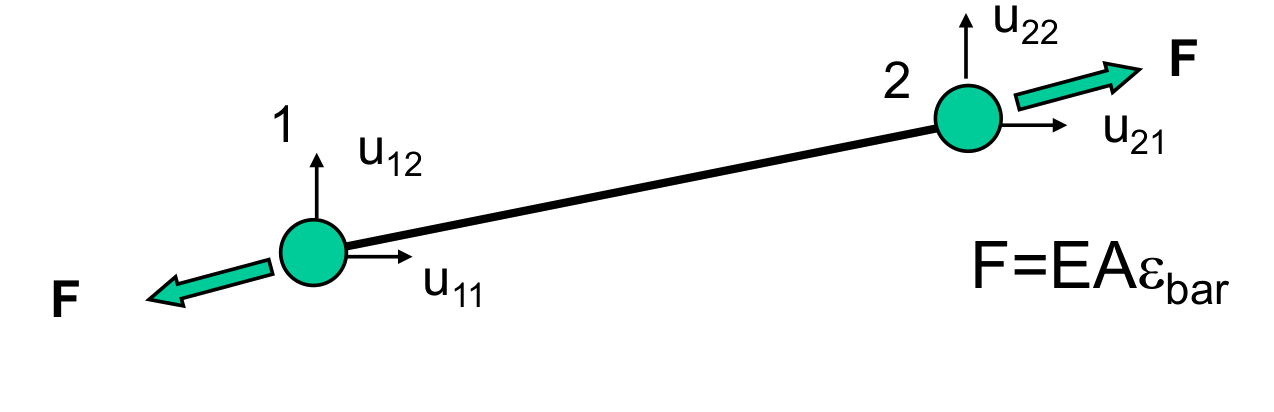
\includegraphics[width=0.65\textwidth]{figs/bar-element.png}
\end{figure}
\mode<handout>{
	\vspace{3cm}
}
\end{frame}

\note{
	\begin{enumerate}
		\item Node to Node: are springs that are used to model ties between two points. 
		\item It’s not recommended to draw geometry line at position where node-to-node anchor is to be placed. 
		\item It’s a 2 node elastic spring element with normal stiffness (Spring constant)
		\item Element can sustain both tensile forces (anchors) as well as compressive forces (struts).
		\item Fixed-End anchors:  Modelling of struts or props to sheet pile walls. 
	\end{enumerate}
}

\note{
	\begin{enumerate}
		\item Geogrids are slender structures with a normal stiffness but no bending stifness. 
		\item Geogrids can only sustain \textbf{Tensile forces} and no compression!
		\item Structures involving geotextiles. 
	\end{enumerate}
	\begin{figure}[ht]
		\centering
		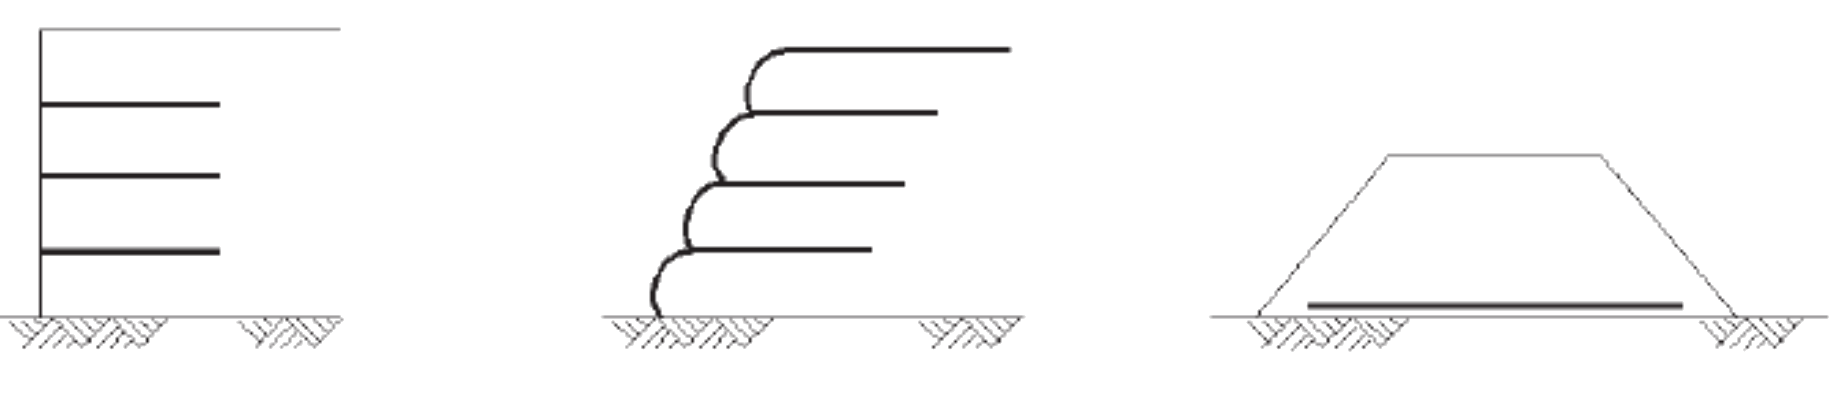
\includegraphics[width=0.85\textwidth]{figs/geogrids.png}
	\end{figure}
}

%------------------------------------------------
\begin{frame}
\frametitle{1D Finite Elements: Beam element}
two node structure element with axial and bending stiffness (no
transverse shear deformation). Three degrees of freedom for 2D beam element (1, 2
displacements and a moment). \mode<beamer>{Examples are sheet pile walls, structural foundation
	beams, structural facing for reinforced soil walls.}
\begin{figure}[h]
	\centering
	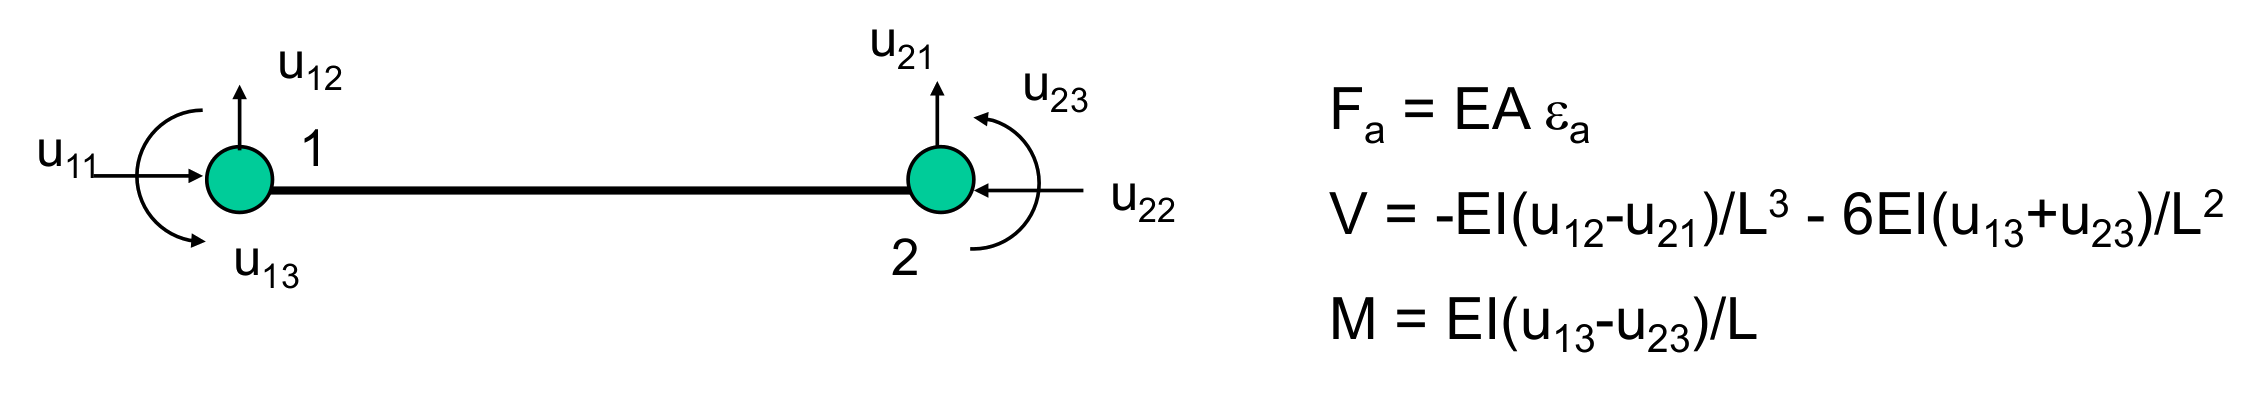
\includegraphics[width=0.75\textwidth]{figs/beam-element.png}
\end{figure}
\begin{figure}[h]
	\centering
	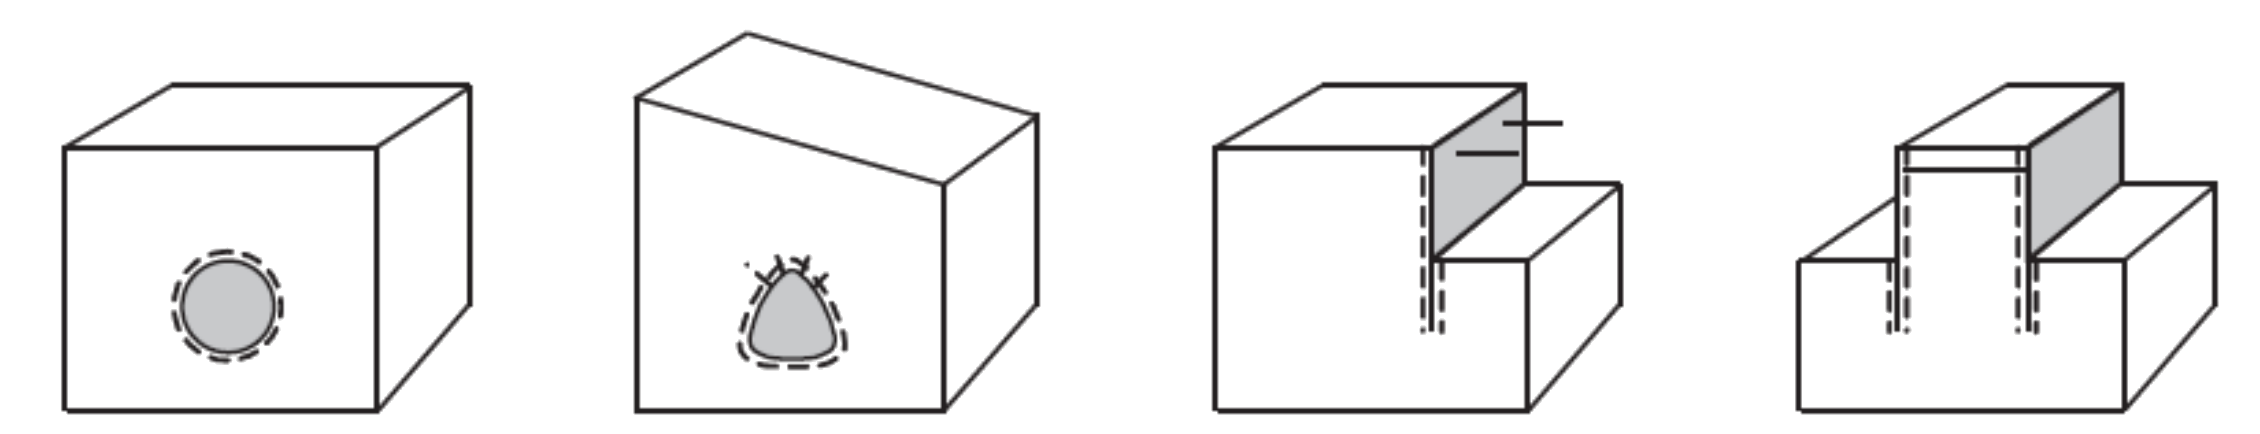
\includegraphics[width=0.75\textwidth]{figs/plate-elements.png}
\end{figure}
\end{frame}

%------------------------------------------------
\begin{frame}
\frametitle{2D plane-strain / axisymmetric elements}
\begin{figure}[ht]
	\centering
	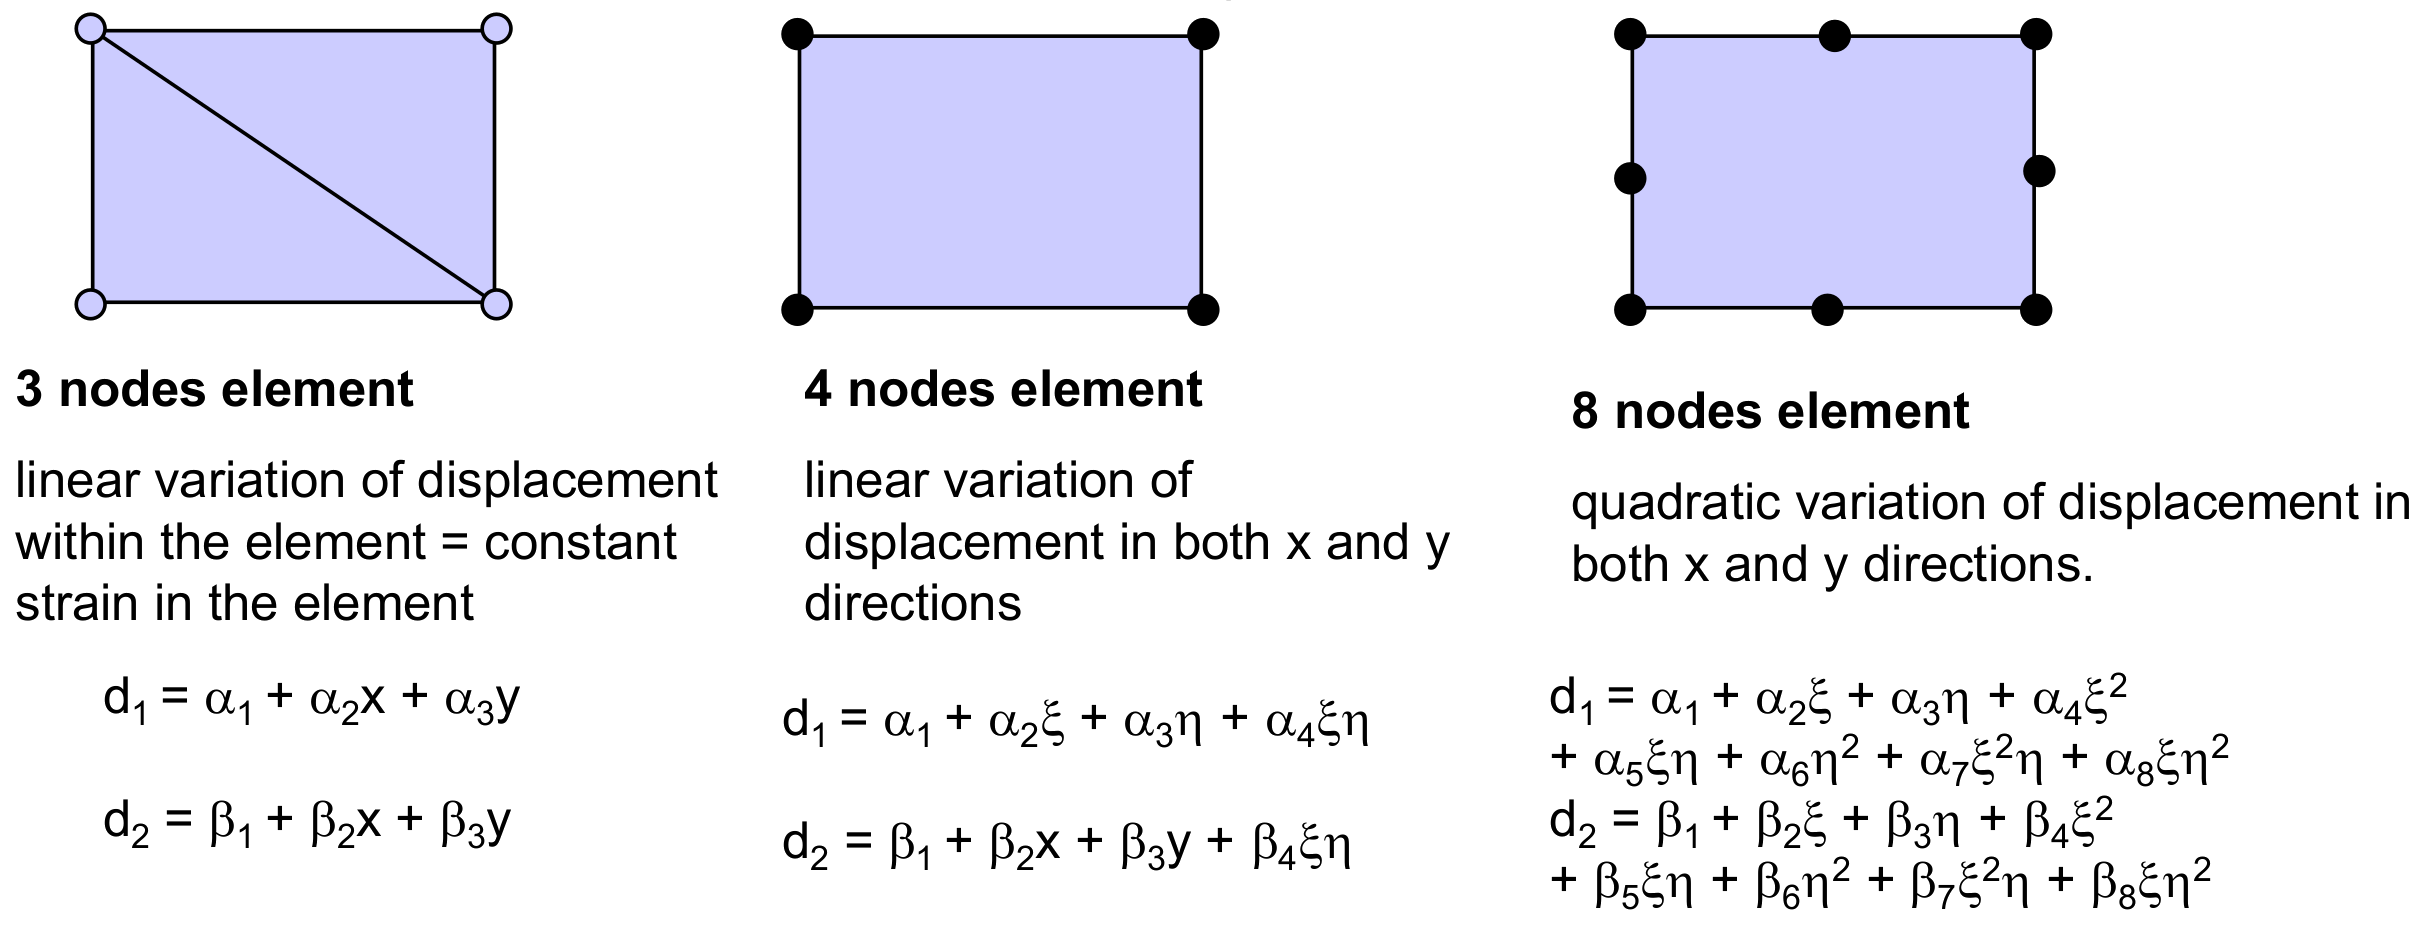
\includegraphics[width=\textwidth]{figs/2d-fe-elements.png}
\end{figure}
\end{frame}

%------------------------------------------------
\begin{frame}
\frametitle{2D/3D Finite elements}
\begin{figure}[ht]
	\centering
	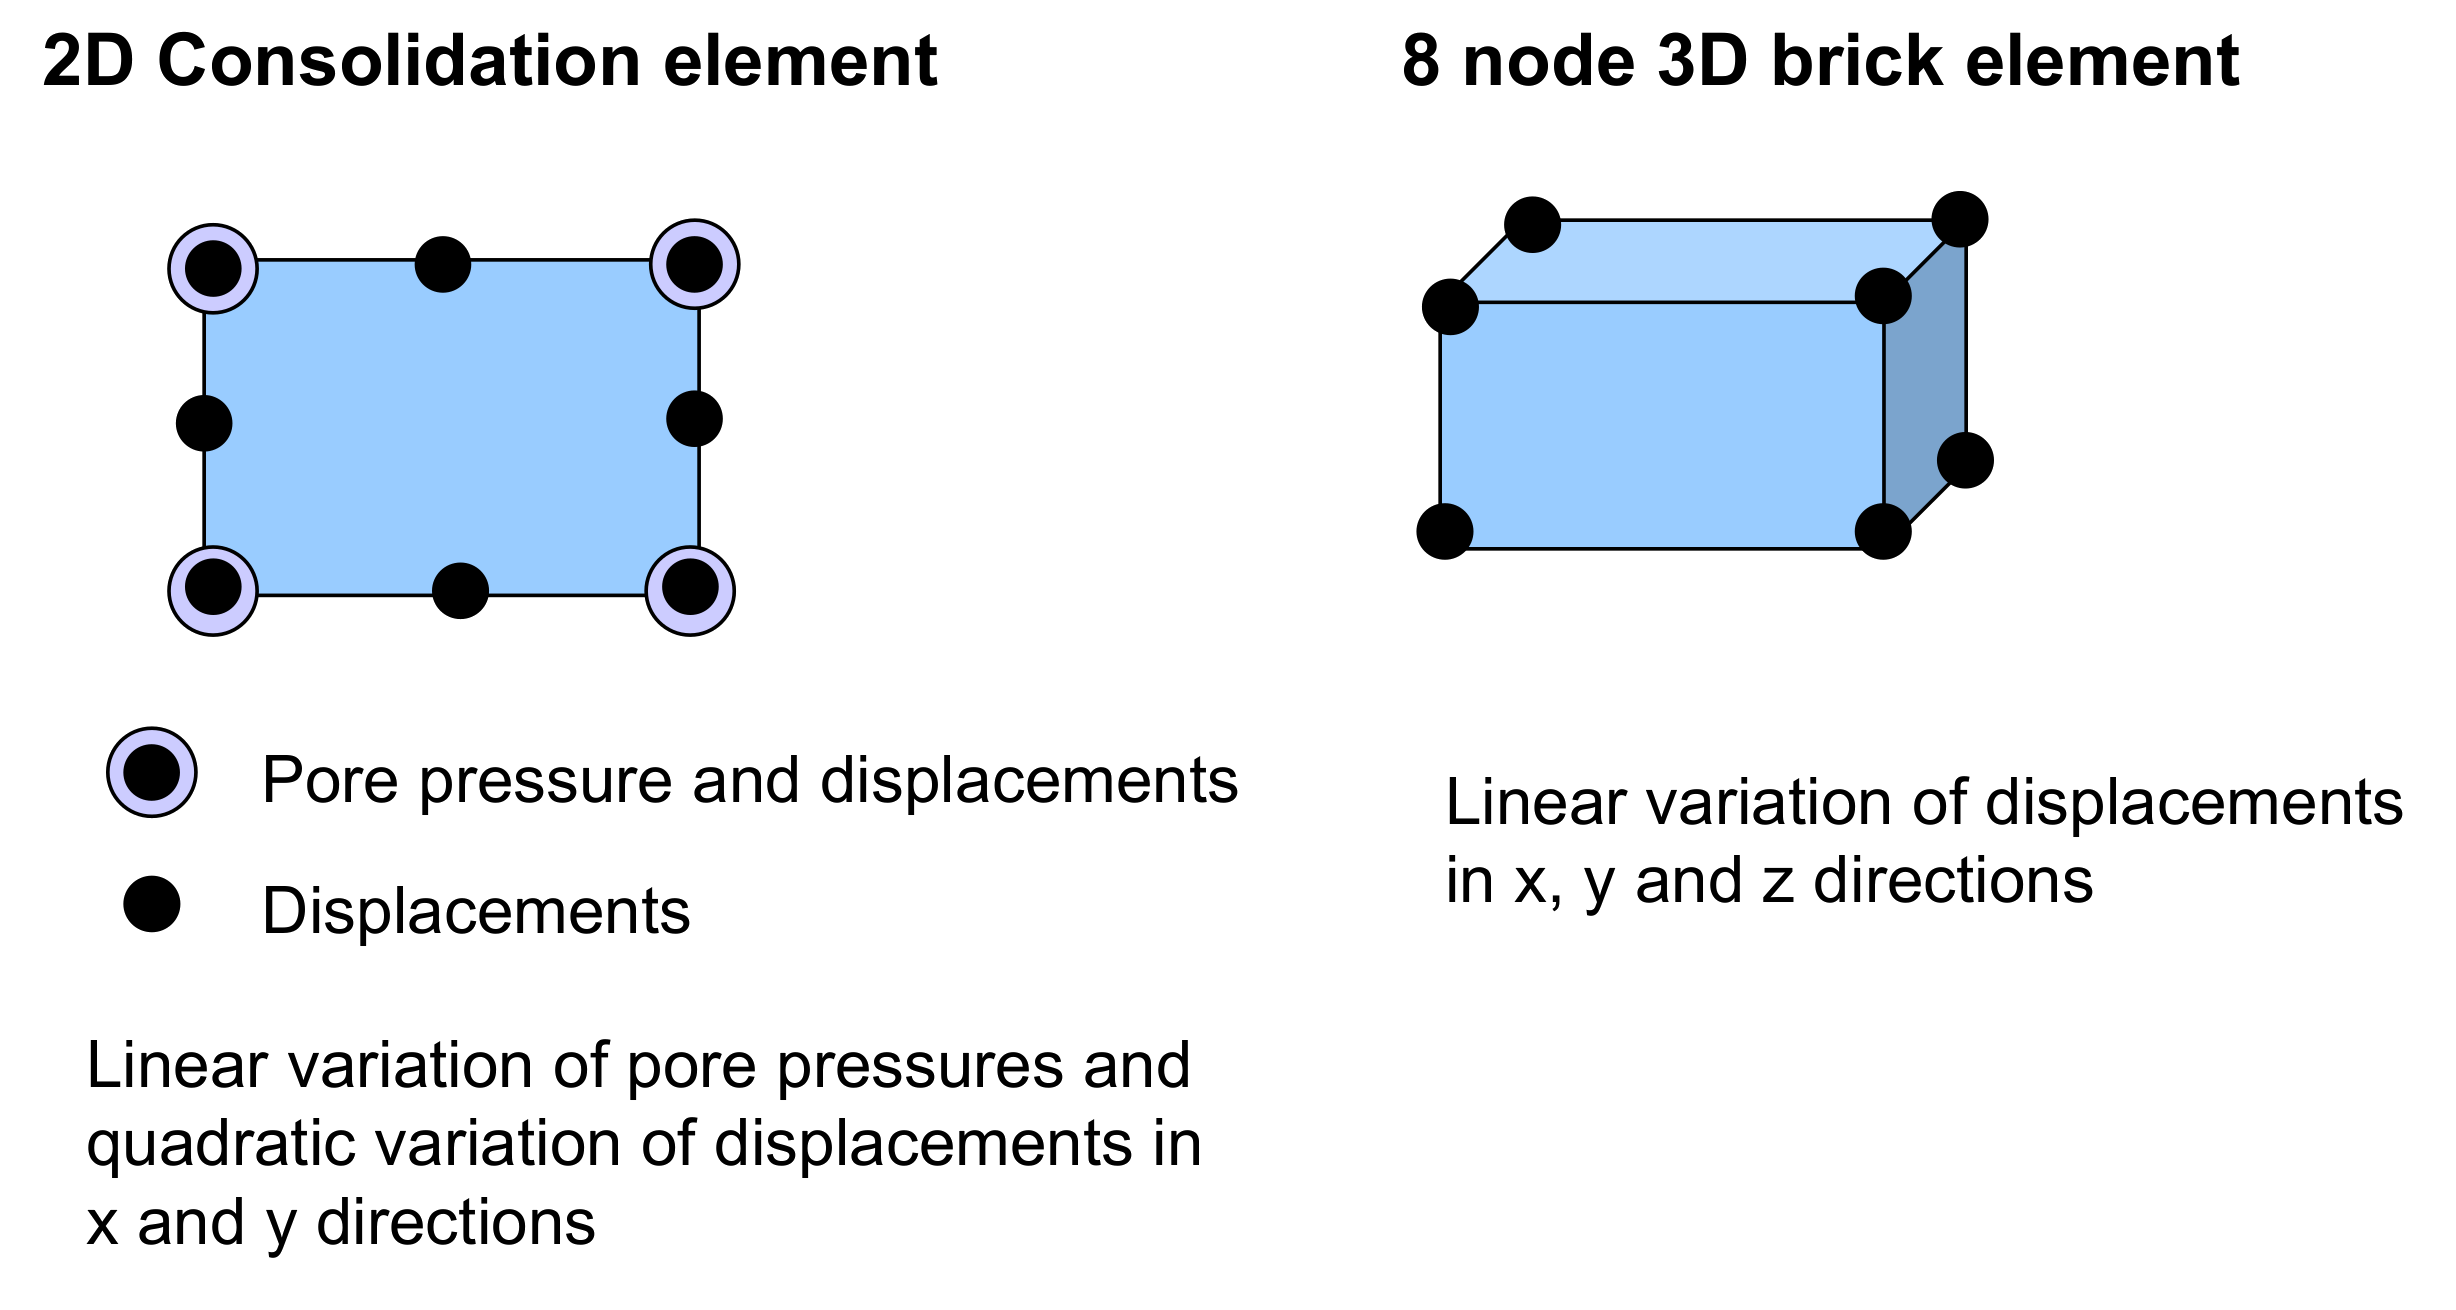
\includegraphics[width=\textwidth]{figs/2d-3d-elements.png}
\end{figure}
\end{frame}

%------------------------------------------------
\begin{frame}
\frametitle{Interface element}
\begin{figure}[ht]
	\centering
	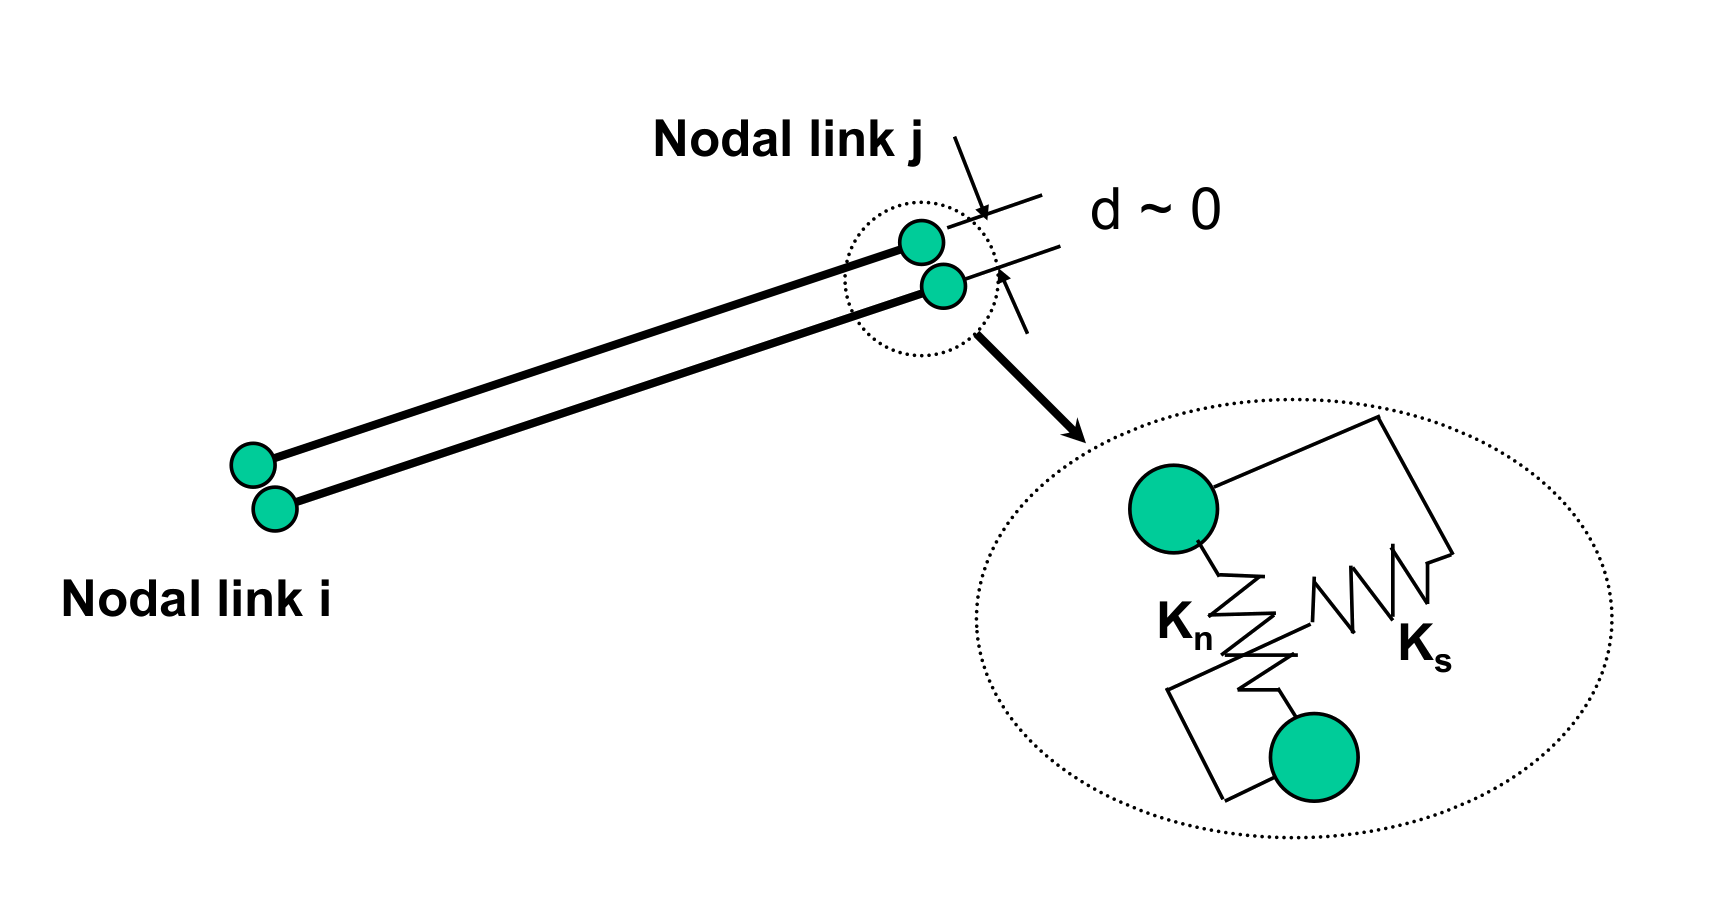
\includegraphics[width=0.5\textwidth]{figs/interface-element.png}
\end{figure}
\begin{figure}[ht]
	\centering
	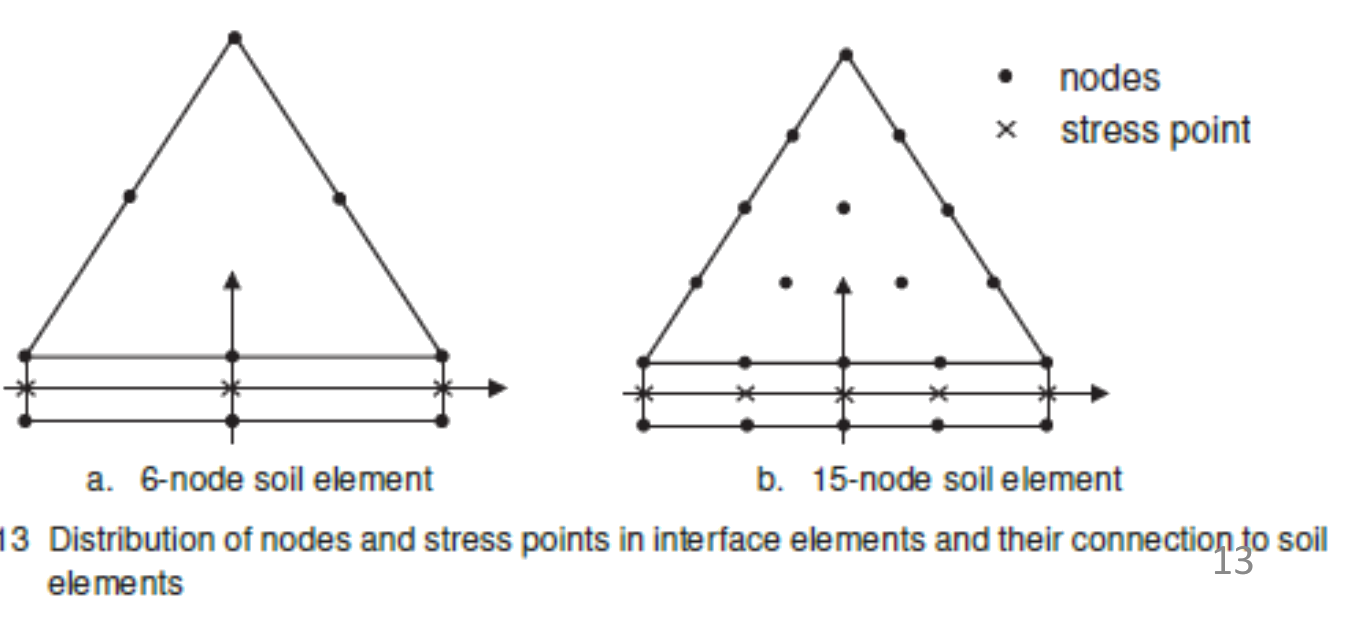
\includegraphics[width=0.6\textwidth]{figs/fe-interface.png}
	\caption*{Use a reduced strength at the interface}
\end{figure}
\end{frame}

\note{This element allows relative displacement between
elements. It is capable to model soil/structure interface conditions, shear planes
within a soil mass. The element is ‘fictitious’ four node element made up of two
independent nodal links. Each link consists of two nodes connected by a normal
and shear spring as shown below. The stiffness of the springs can be non-linear,
modelling frictional slip behaviour. The thickness of the element is assumed to be
negligibles}

%------------------------------------------------
\begin{frame}
\frametitle{Interface elements for Soil Structure Interactions}
\begin{figure}[ht]
	\centering
	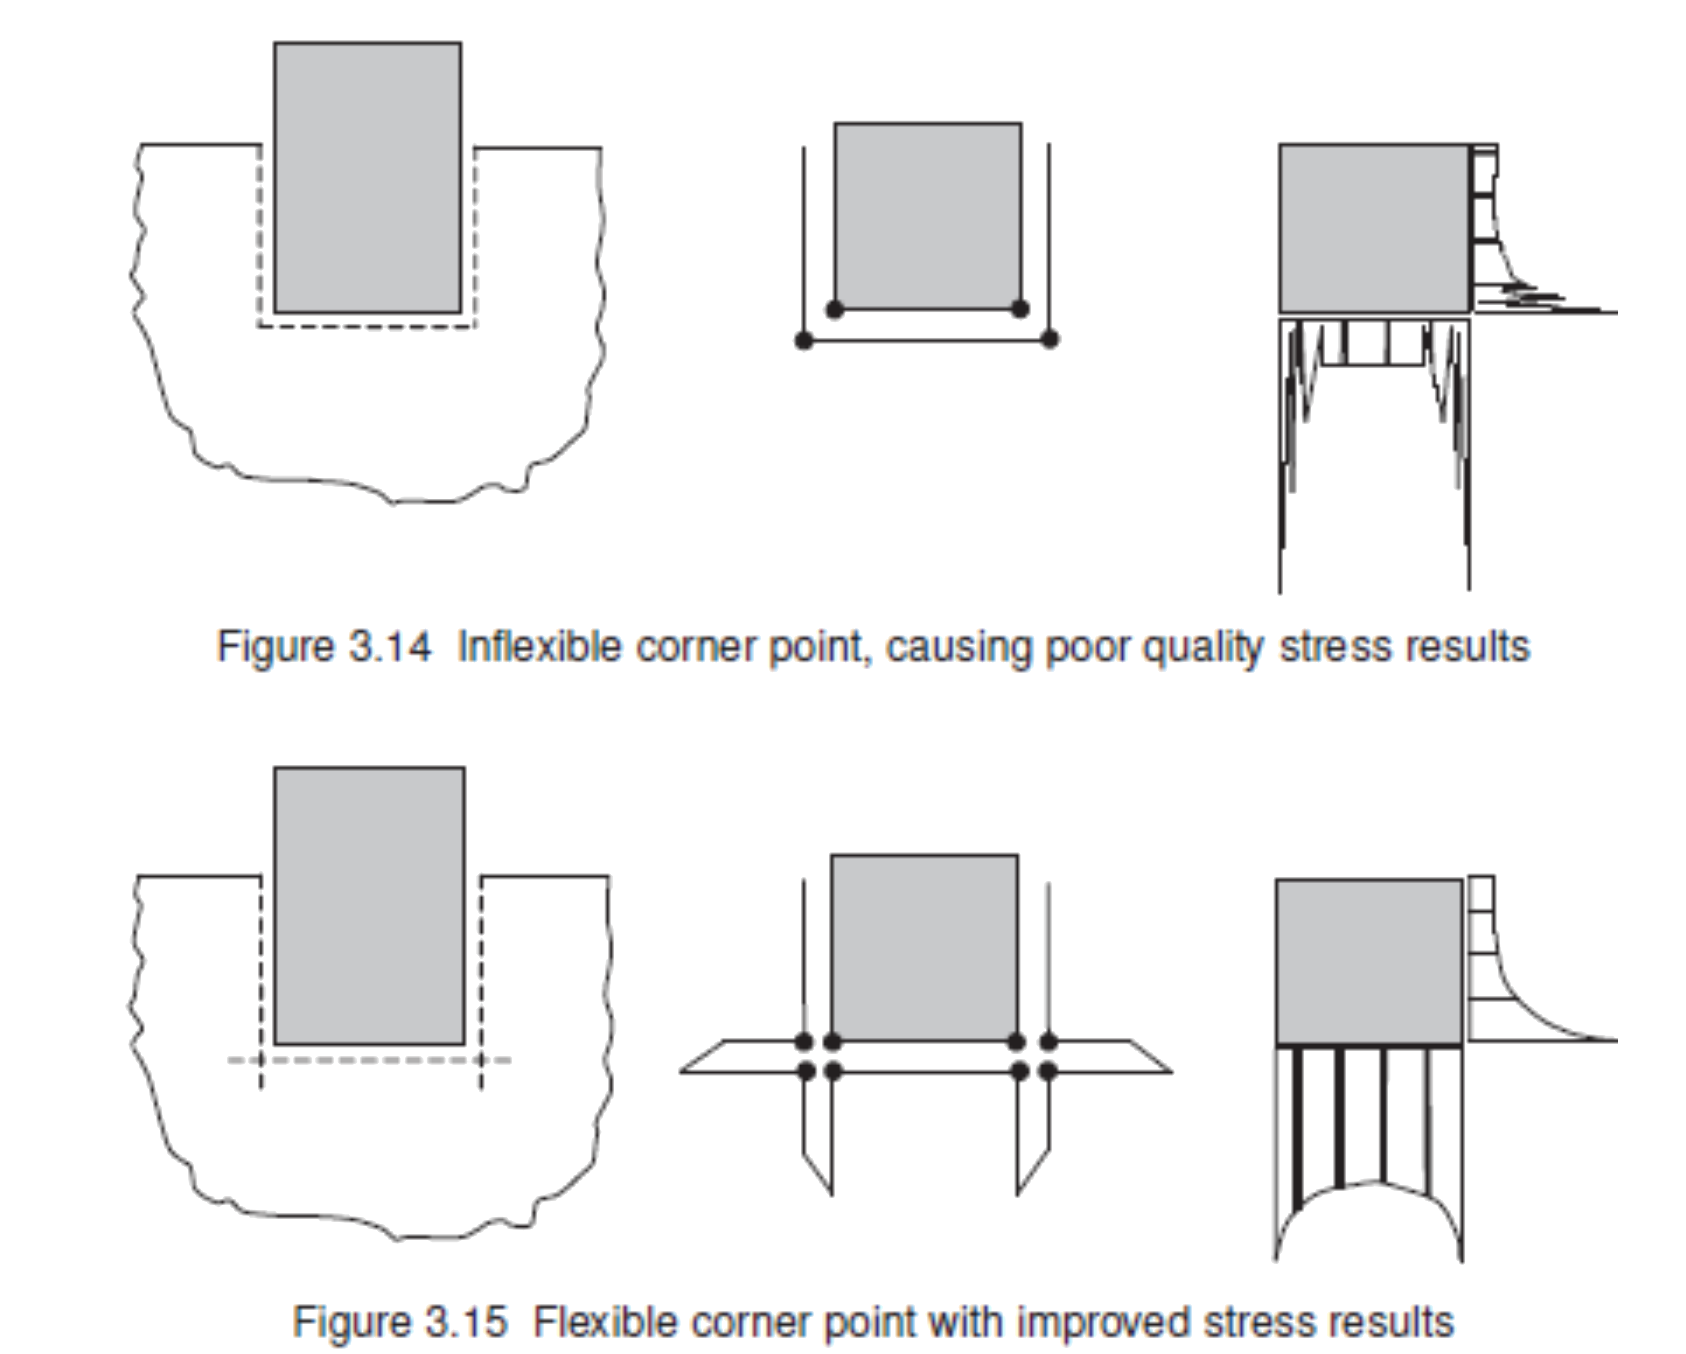
\includegraphics[width=0.65\textwidth]{figs/interface-ssi.png}
\end{figure}
\end{frame}

\subsection{Discretization}
%------------------------------------------------
\begin{frame}
\frametitle{FE discretization}
\begin{figure}[ht]
	\centering
	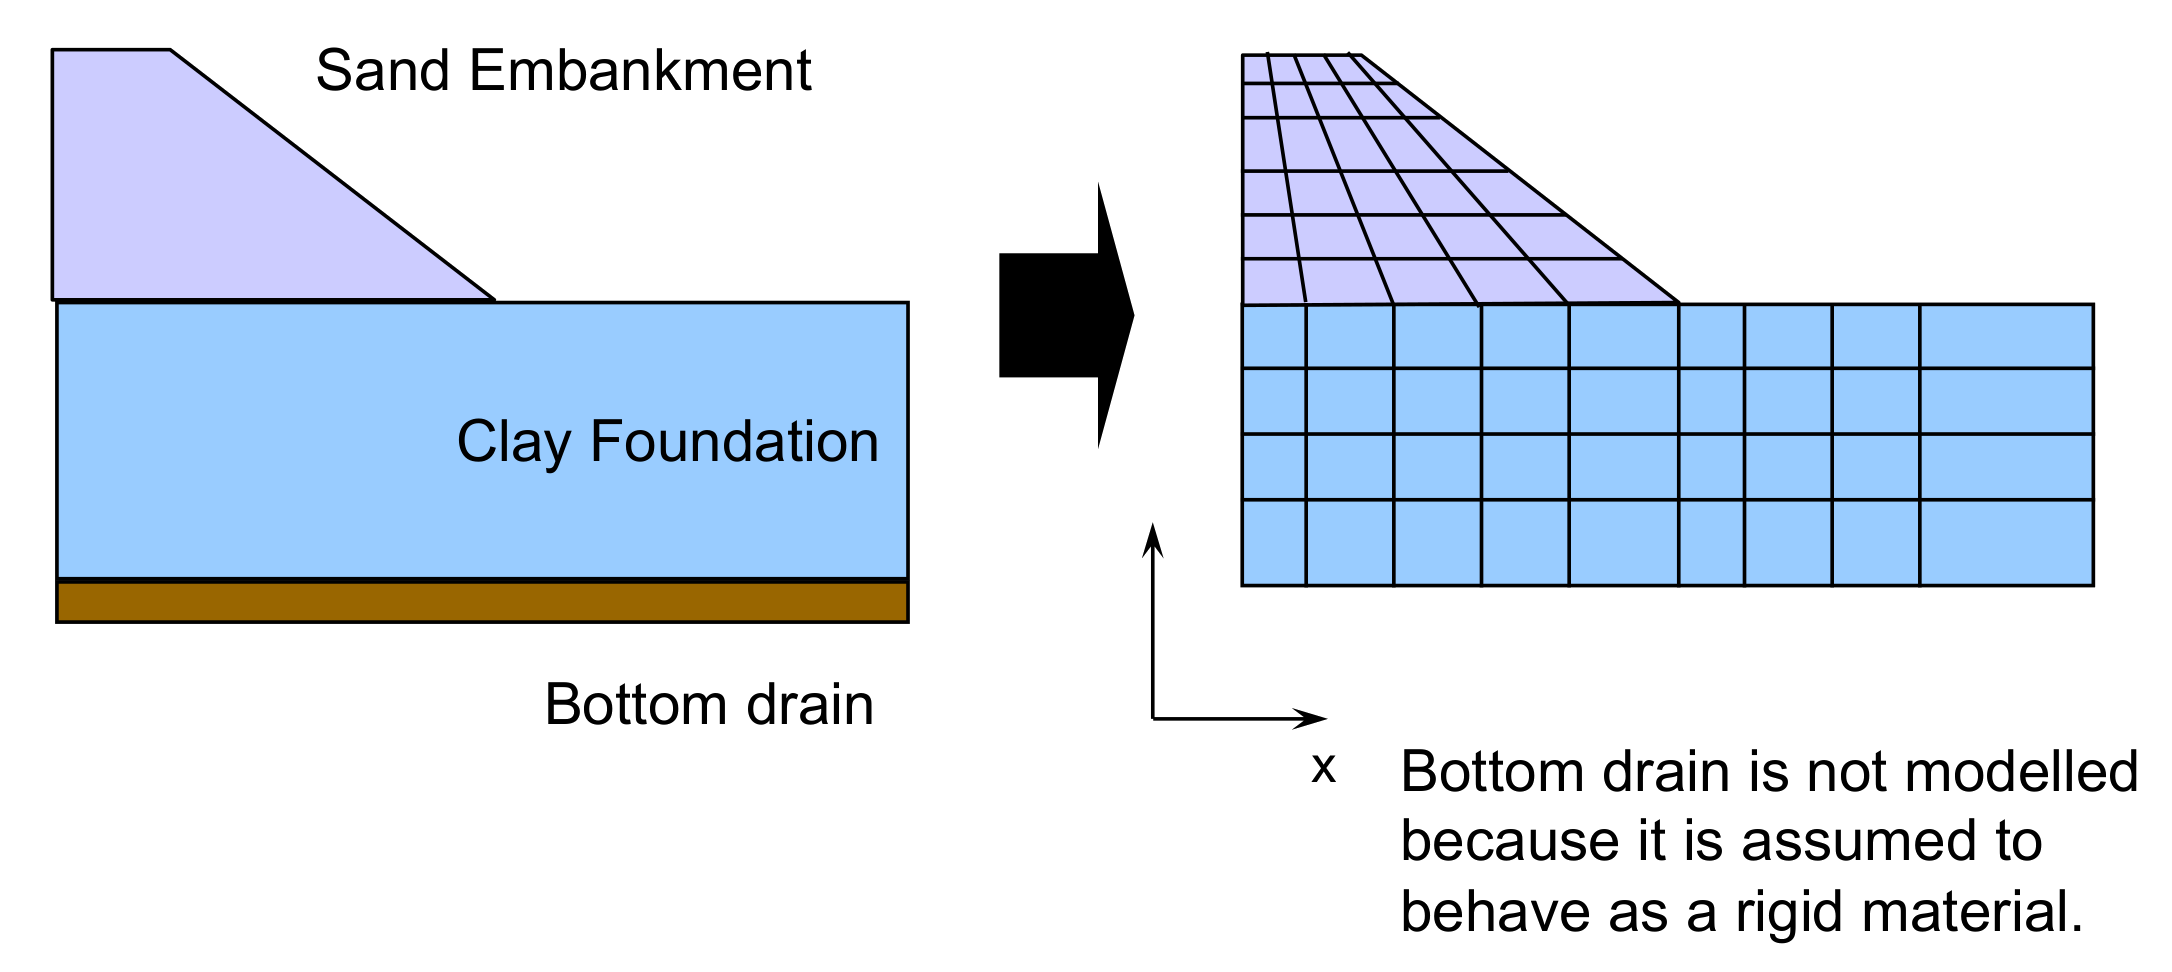
\includegraphics[width=\textwidth]{figs/discretization.png}
\end{figure}
\end{frame}

%------------------------------------------------
\begin{frame}
\frametitle{FE discretization}
\begin{figure}[ht]
	\centering
	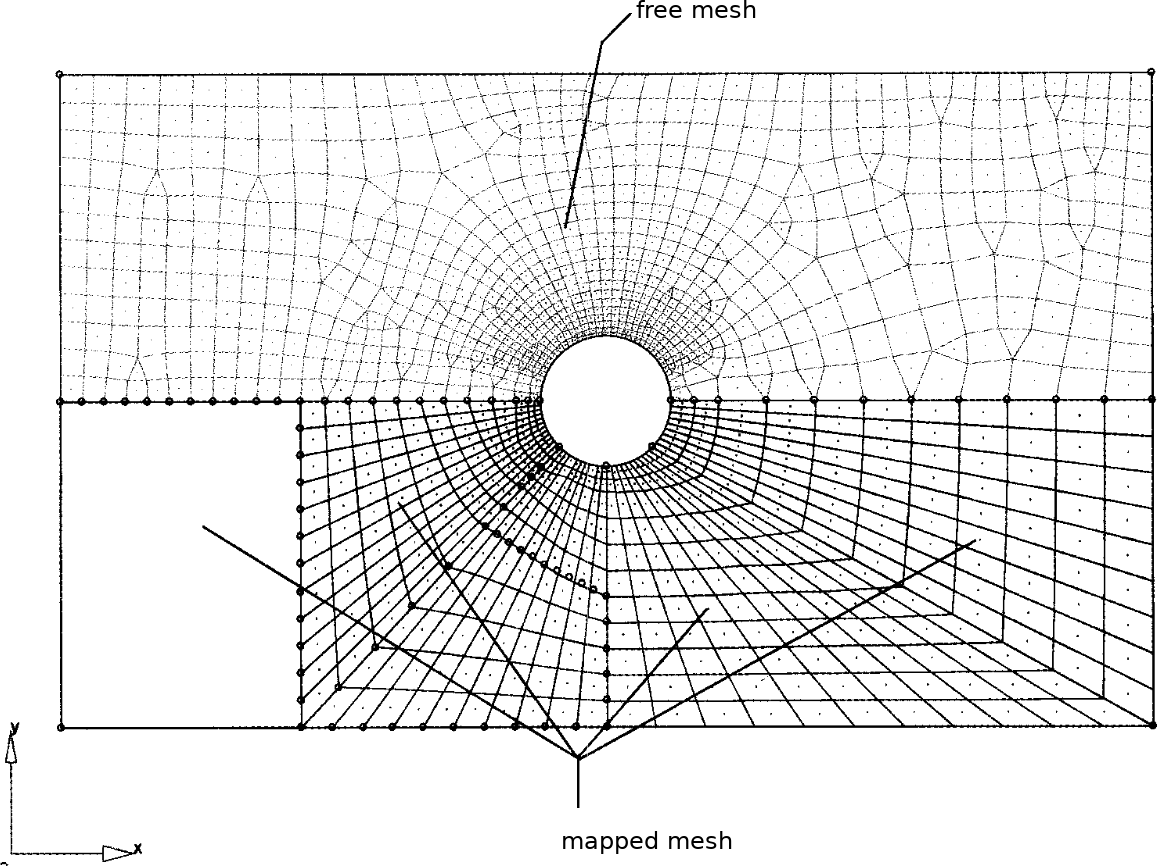
\includegraphics[width=0.8\textwidth]{figs/mesh-discretization.png}
\end{figure}
\end{frame}

\note{
	There are many algorithms to generate mesh for a given object. The top part of the geometry is a
	mesh generated by ``\textit{free meshing}'', in which elements are generated automatically with triangles
	and quadrilaterals within the whole domain. The bottom part of the geometry is a mesh generated by
	``\textit{mapped meshing}'', in which quadrilateral elements are placed in subzones with a more regular
	manner. The mesh density is also more controlled.\\
	
	Some elements generated in the previous figure show that the interior nodes are shared by
	more than one element. The number of elements that share a node is called valence. The
	ideal valence of interior nodes for quadrilaterals is four to achieve the optimum interior angle
	of 90 degrees. For triangles, it is six. After a mesh is generated, it is ideal to clean up the
	mesh.
}

%------------------------------------------------
\begin{frame}
\frametitle{FE discretization}
	
\noindent
\fboxsep=0pt
\noindent
\begin{minipage}[t]{0.49\linewidth}
	\begin{figure}
		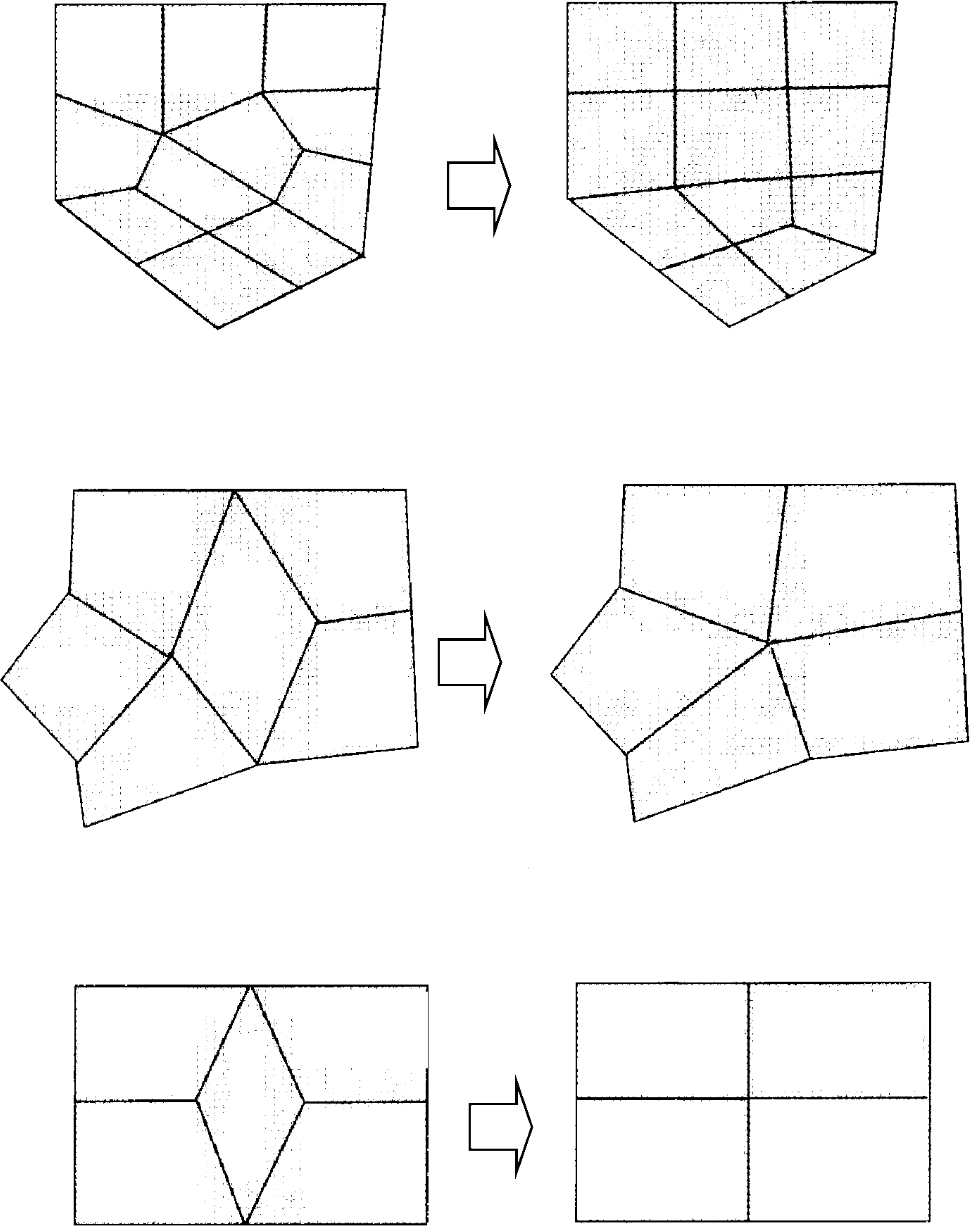
\includegraphics[width=\textwidth]{figs/element-repair.png}
	\end{figure}
\end{minipage}%
\hfill%
\begin{minipage}[t]{0.49\linewidth}
	\begin{enumerate}
		\item Node valence less or equal to two and greater than or equal to
		six should be eliminated.
		\item The number of nodes with valence of three or five should be
		minimized.
		\item Angles greater than 160 degrees should be eliminated.
		\item The aspect ratio should be less than 3 for stress analysis and
		10 for displacement analysis.
	\end{enumerate}
\end{minipage}	
\end{frame}

\note{
	\begin{itemize}
		\item A square element is ideal. 
		\item Minimize ``\textit{skew}'': $\left|\left|\mathrm{angle} - 90\deg\right|\right|$
		\item Minimize aspect ratio: $\frac{\left|\left|\mathrm{longest edge}\right|
			\right|}{\left|\left|\mathrm{shortest edge}\right|
			\right|}$
		\item Keep bad elements away from the boundary
	\end{itemize}

}


%------------------------------------------------
\begin{frame}
\frametitle{FE discretization}
\begin{figure}[ht]
	\centering
	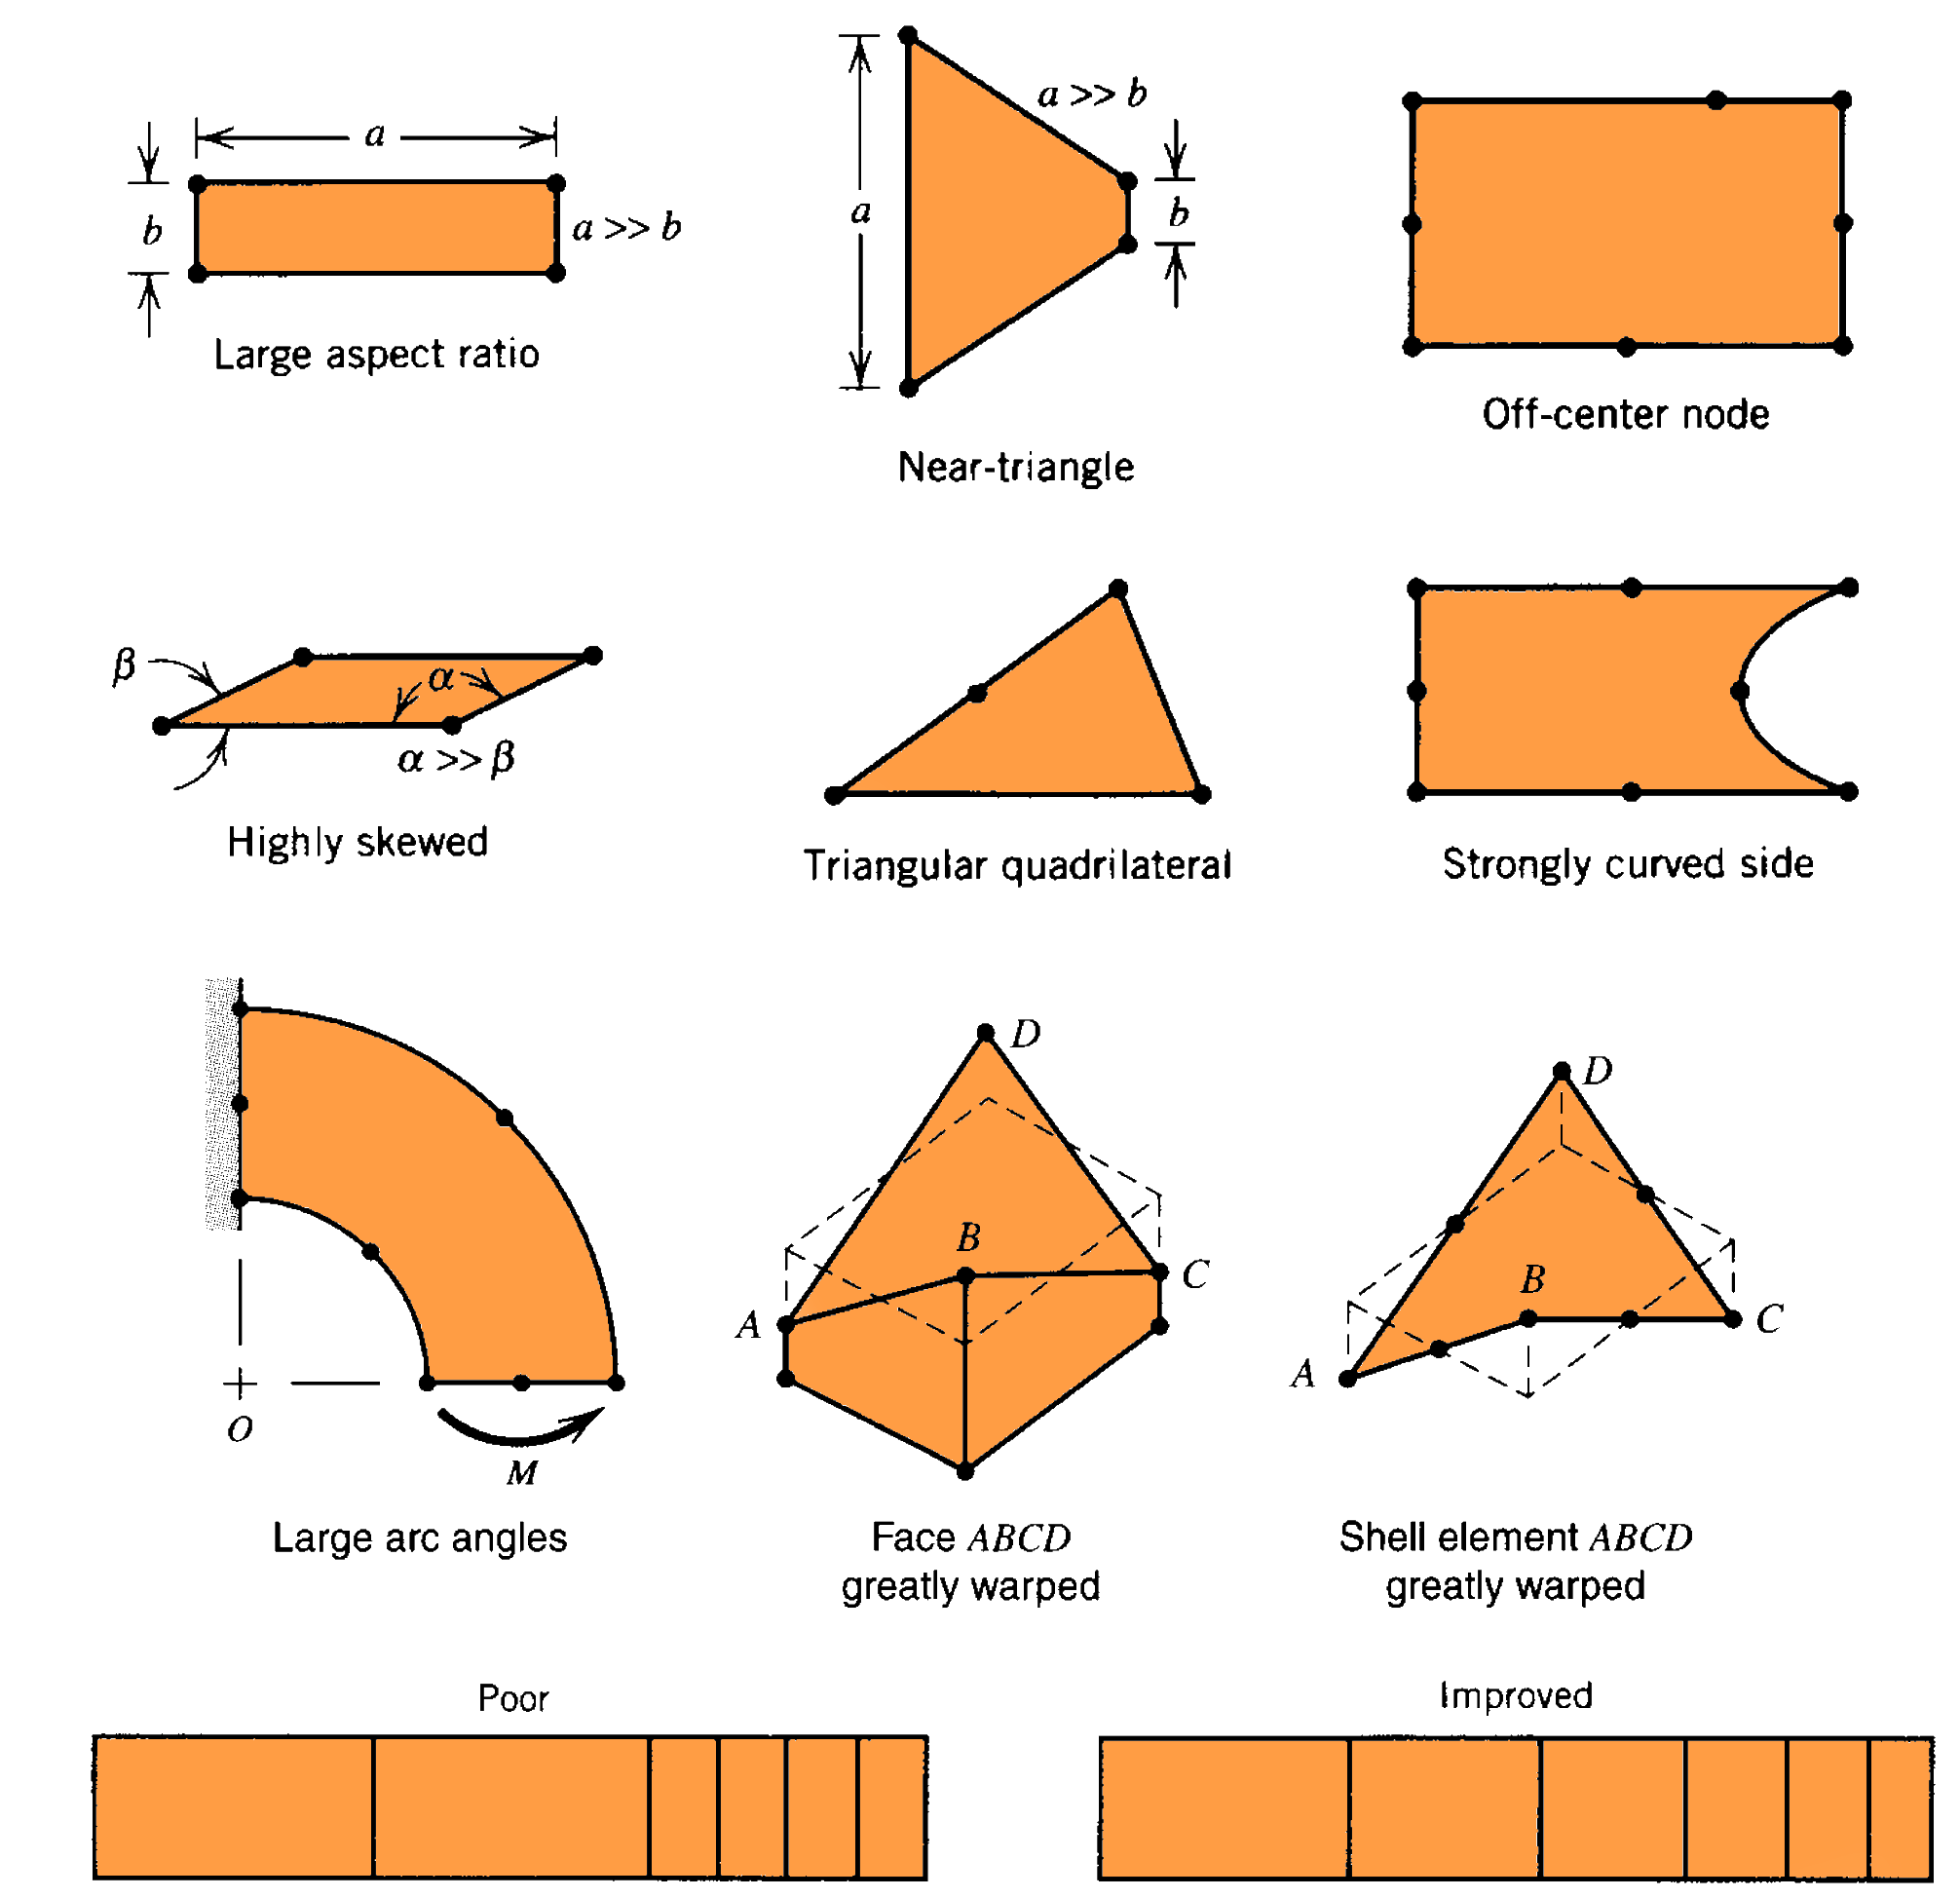
\includegraphics[width=0.8\textwidth]{figs/acceptable-discretization.png}
\end{figure}
\end{frame}

%------------------------------------------------
\begin{frame}
\frametitle{FE discretization}
\mode<beamer>{
	\begin{figure}[ht]
		\centering
		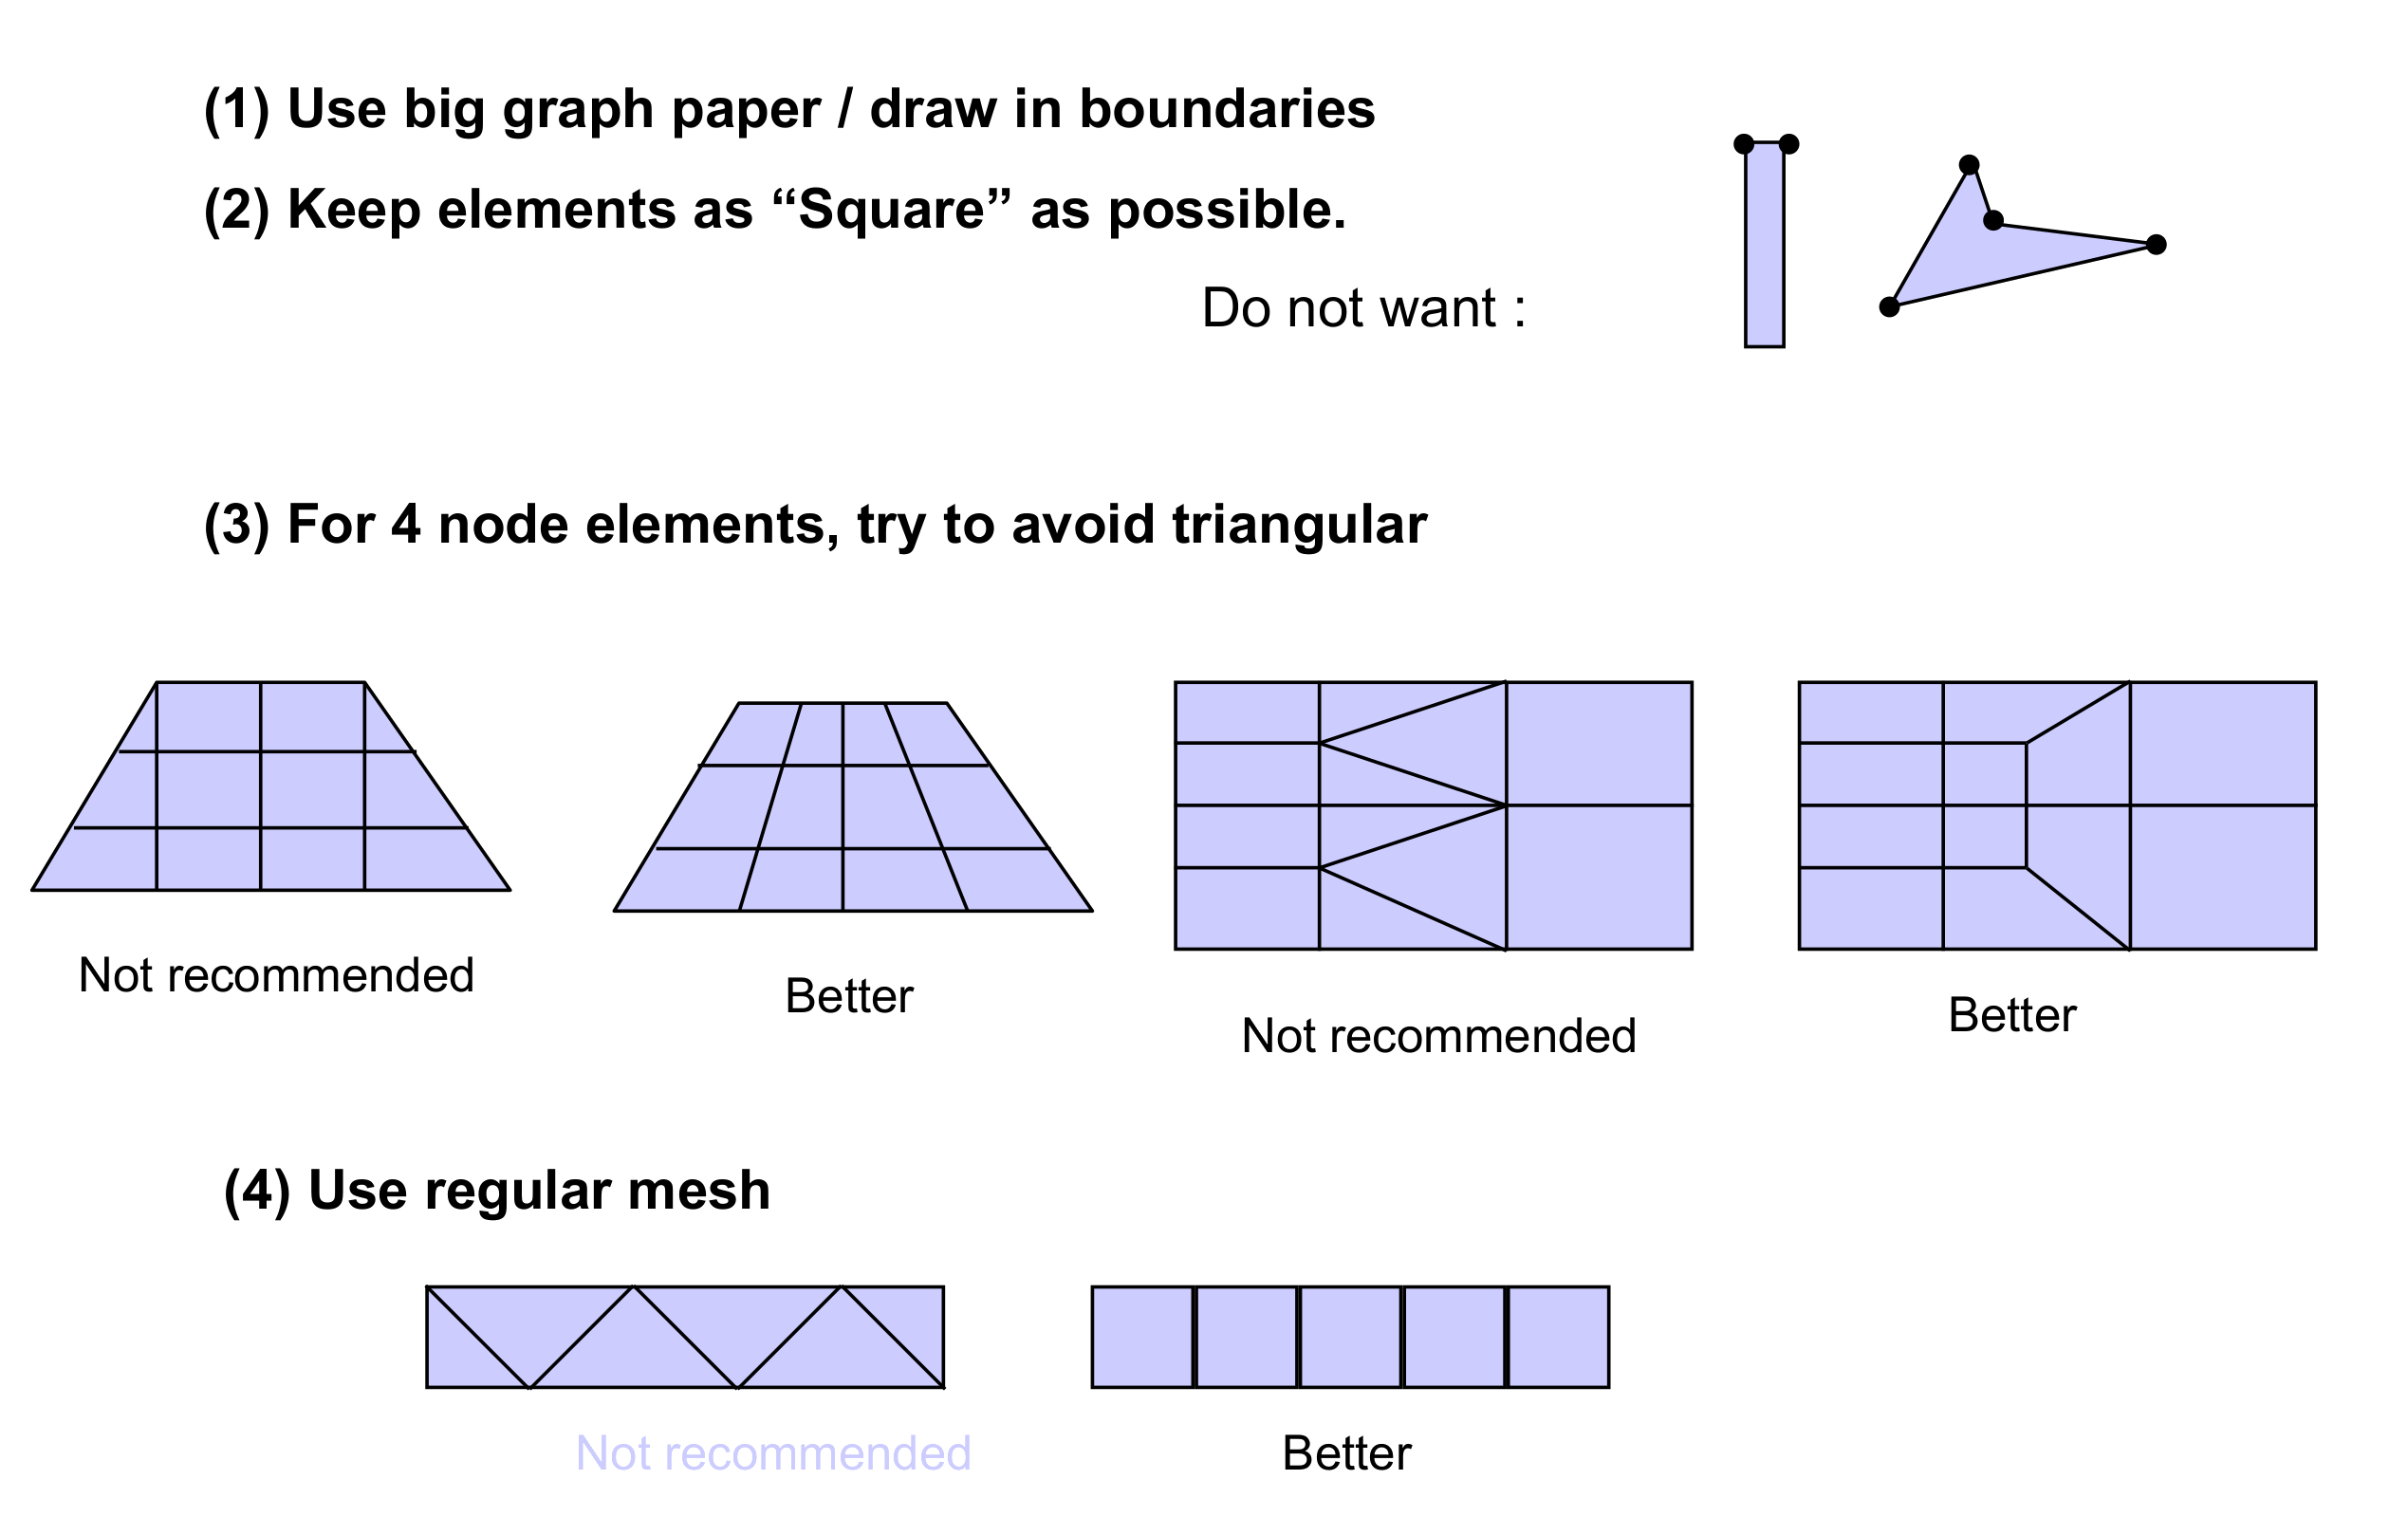
\includegraphics[width=\textwidth]{figs/fe-elements.png}
	\end{figure}
}
\mode<handout>{
	\begin{figure}[ht]
		\centering
		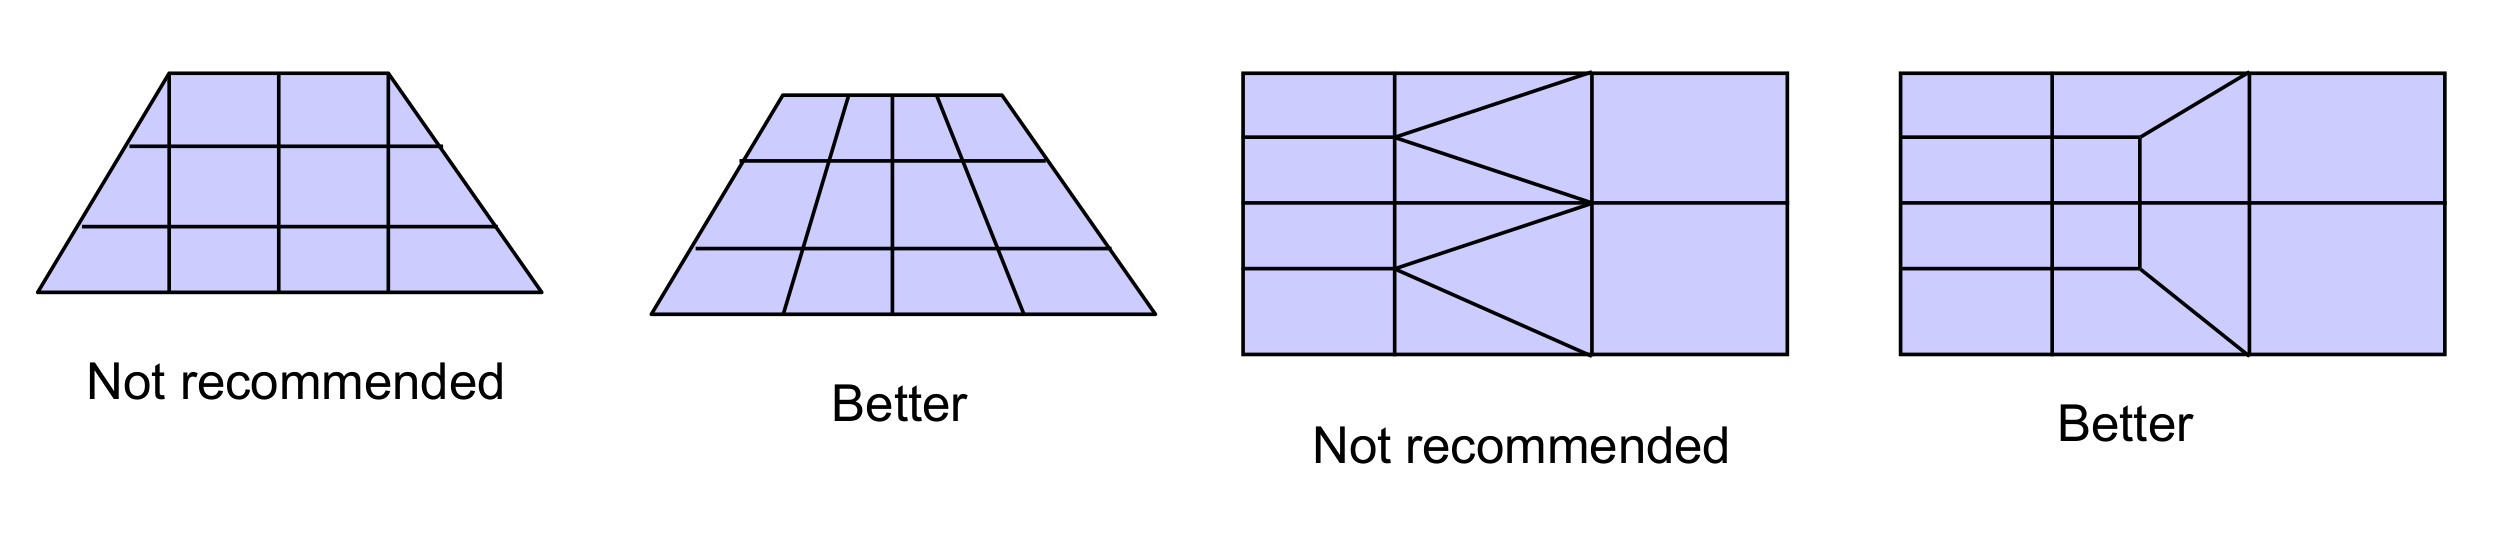
\includegraphics[width=\textwidth]{figs/good-fe-elements.png}
	\end{figure}
	\vspace{4cm}
}
\end{frame}

%------------------------------------------------
\begin{frame}
\frametitle{FE discretization: Refining}
\begin{figure}[ht]
	\centering
	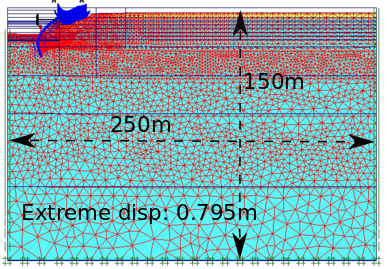
\includegraphics[width=0.8\textwidth]{figs/refined-mesh.png}
	\caption*{Avoid large jumps in element size: size jump should be $< 3$}
\end{figure}
\end{frame}


%------------------------------------------------
\begin{frame}
\frametitle{FE mesh compatibility}

\begin{figure}[ht]
	\centering
	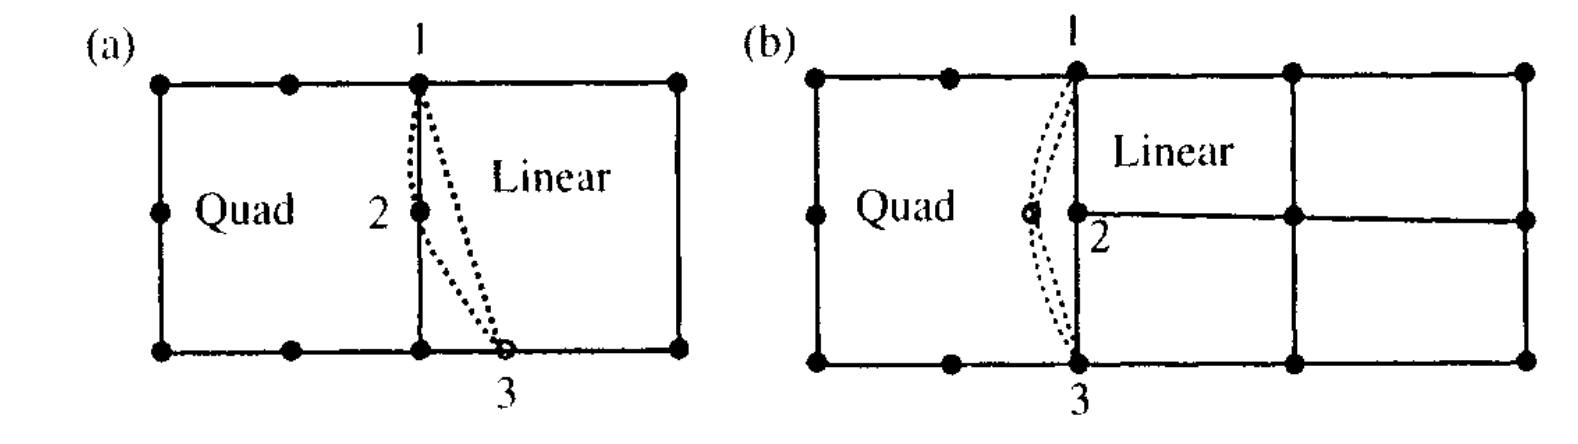
\includegraphics[width=0.75\textwidth]{figs/mesh-incompatibility.png}
	\caption*{Incompatible mesh}
\end{figure}

\mode<beamer>{
	\begin{figure}[ht]
		\centering
		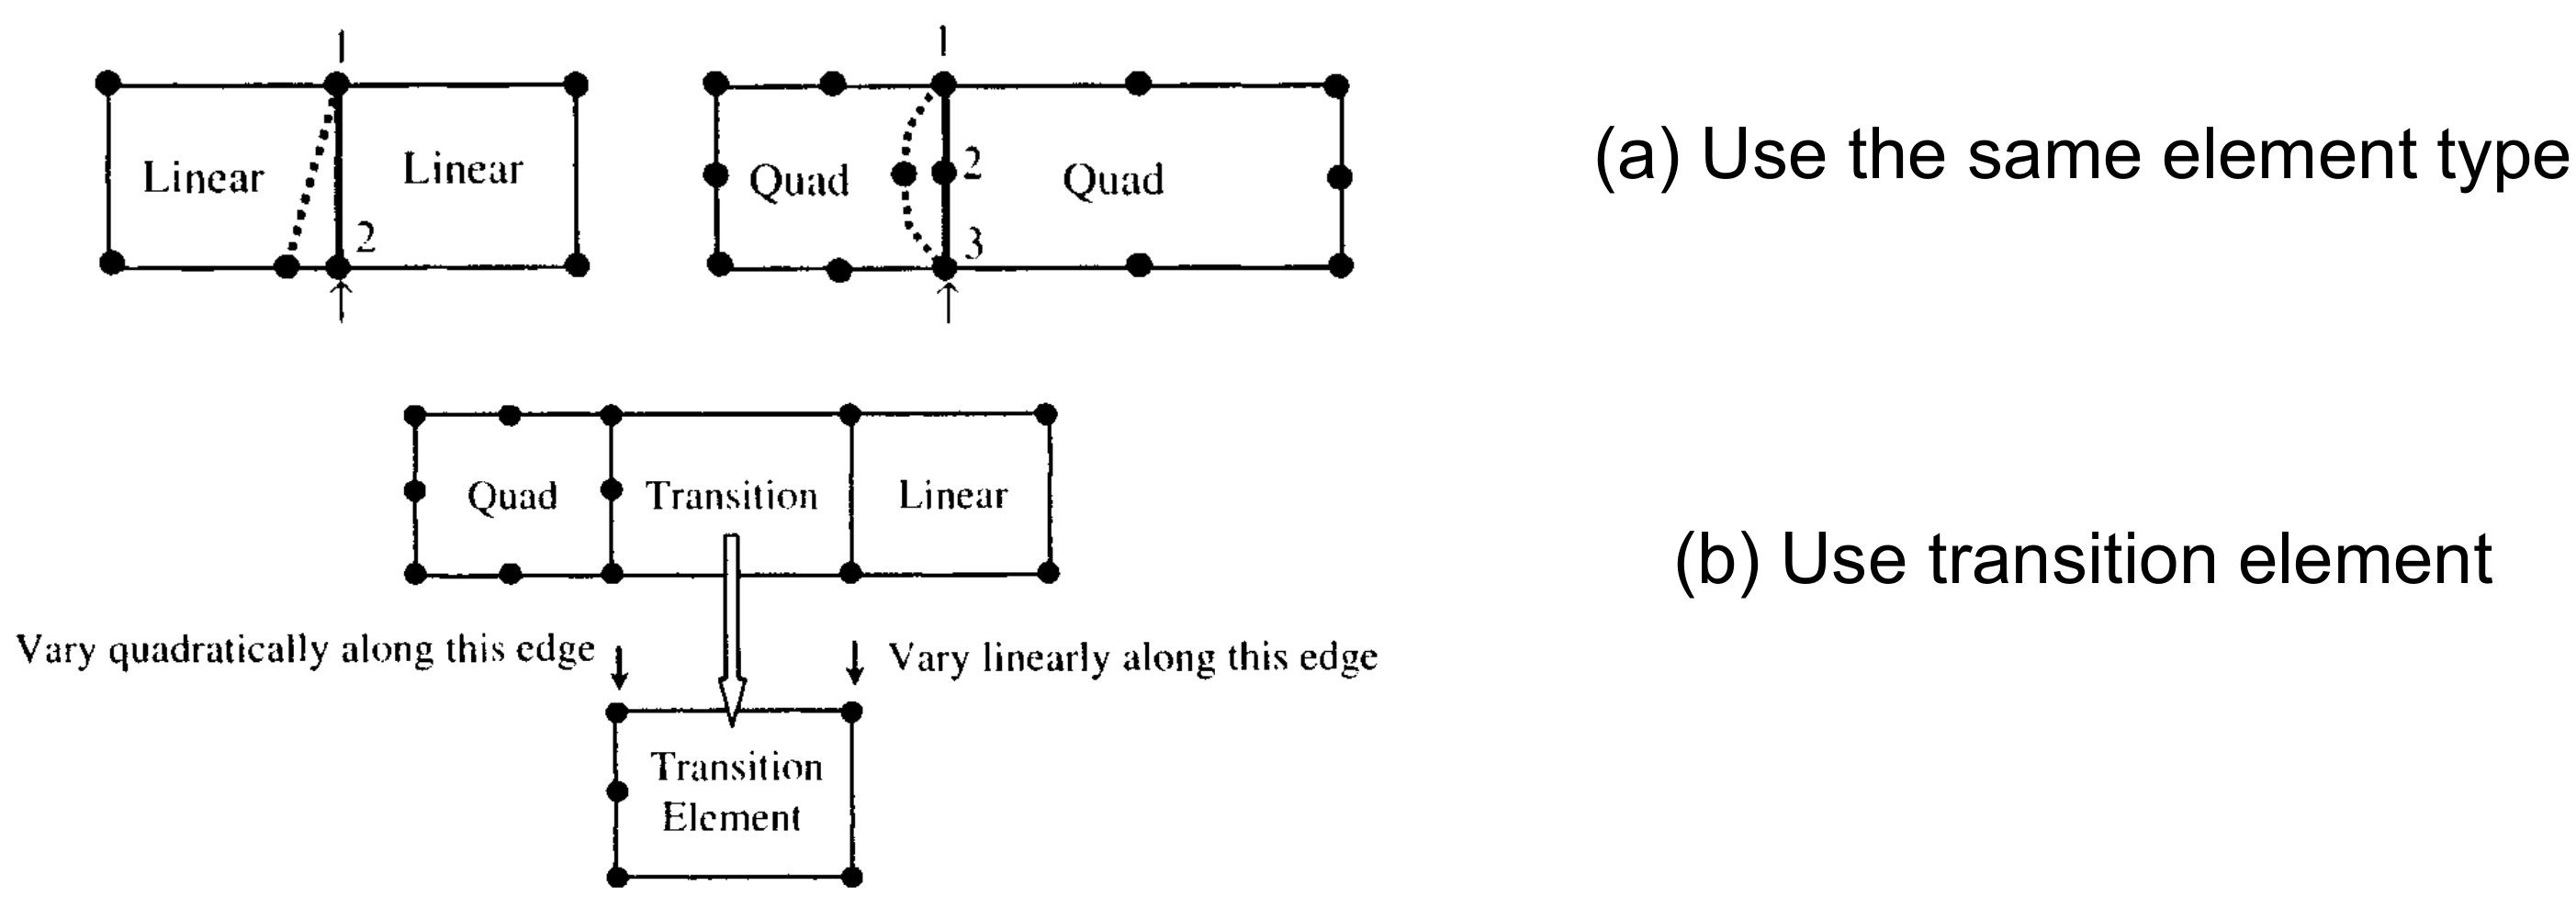
\includegraphics[width=0.75\textwidth]{figs/mesh-compatibility.png}
		\caption*{compatible mesh}
	\end{figure}
}
\mode<handout>{
	\vspace{3cm}
}
\end{frame}

\note{A mesh is said to be ‘compatible’ if the unknown variables are continuous along all edges
	between all the elements in the mesh. The use of different types of elements in the same
	mesh or improper connection of elements can result in an incompatible mesh. The examples
	of this problem are given in Fig. 1. Solutions of this problem are (i) use the same type of
	elements throughout the entire domain (Fig. 2(a)) or (ii) use transitional elements whose
	shape functions have different orders on different edges (Fig. 2(b)).}


\subsection{Boundary conditions}
%------------------------------------------------
\begin{frame}
\frametitle{FE boundary conditions}
\begin{figure}[ht]
	\centering
	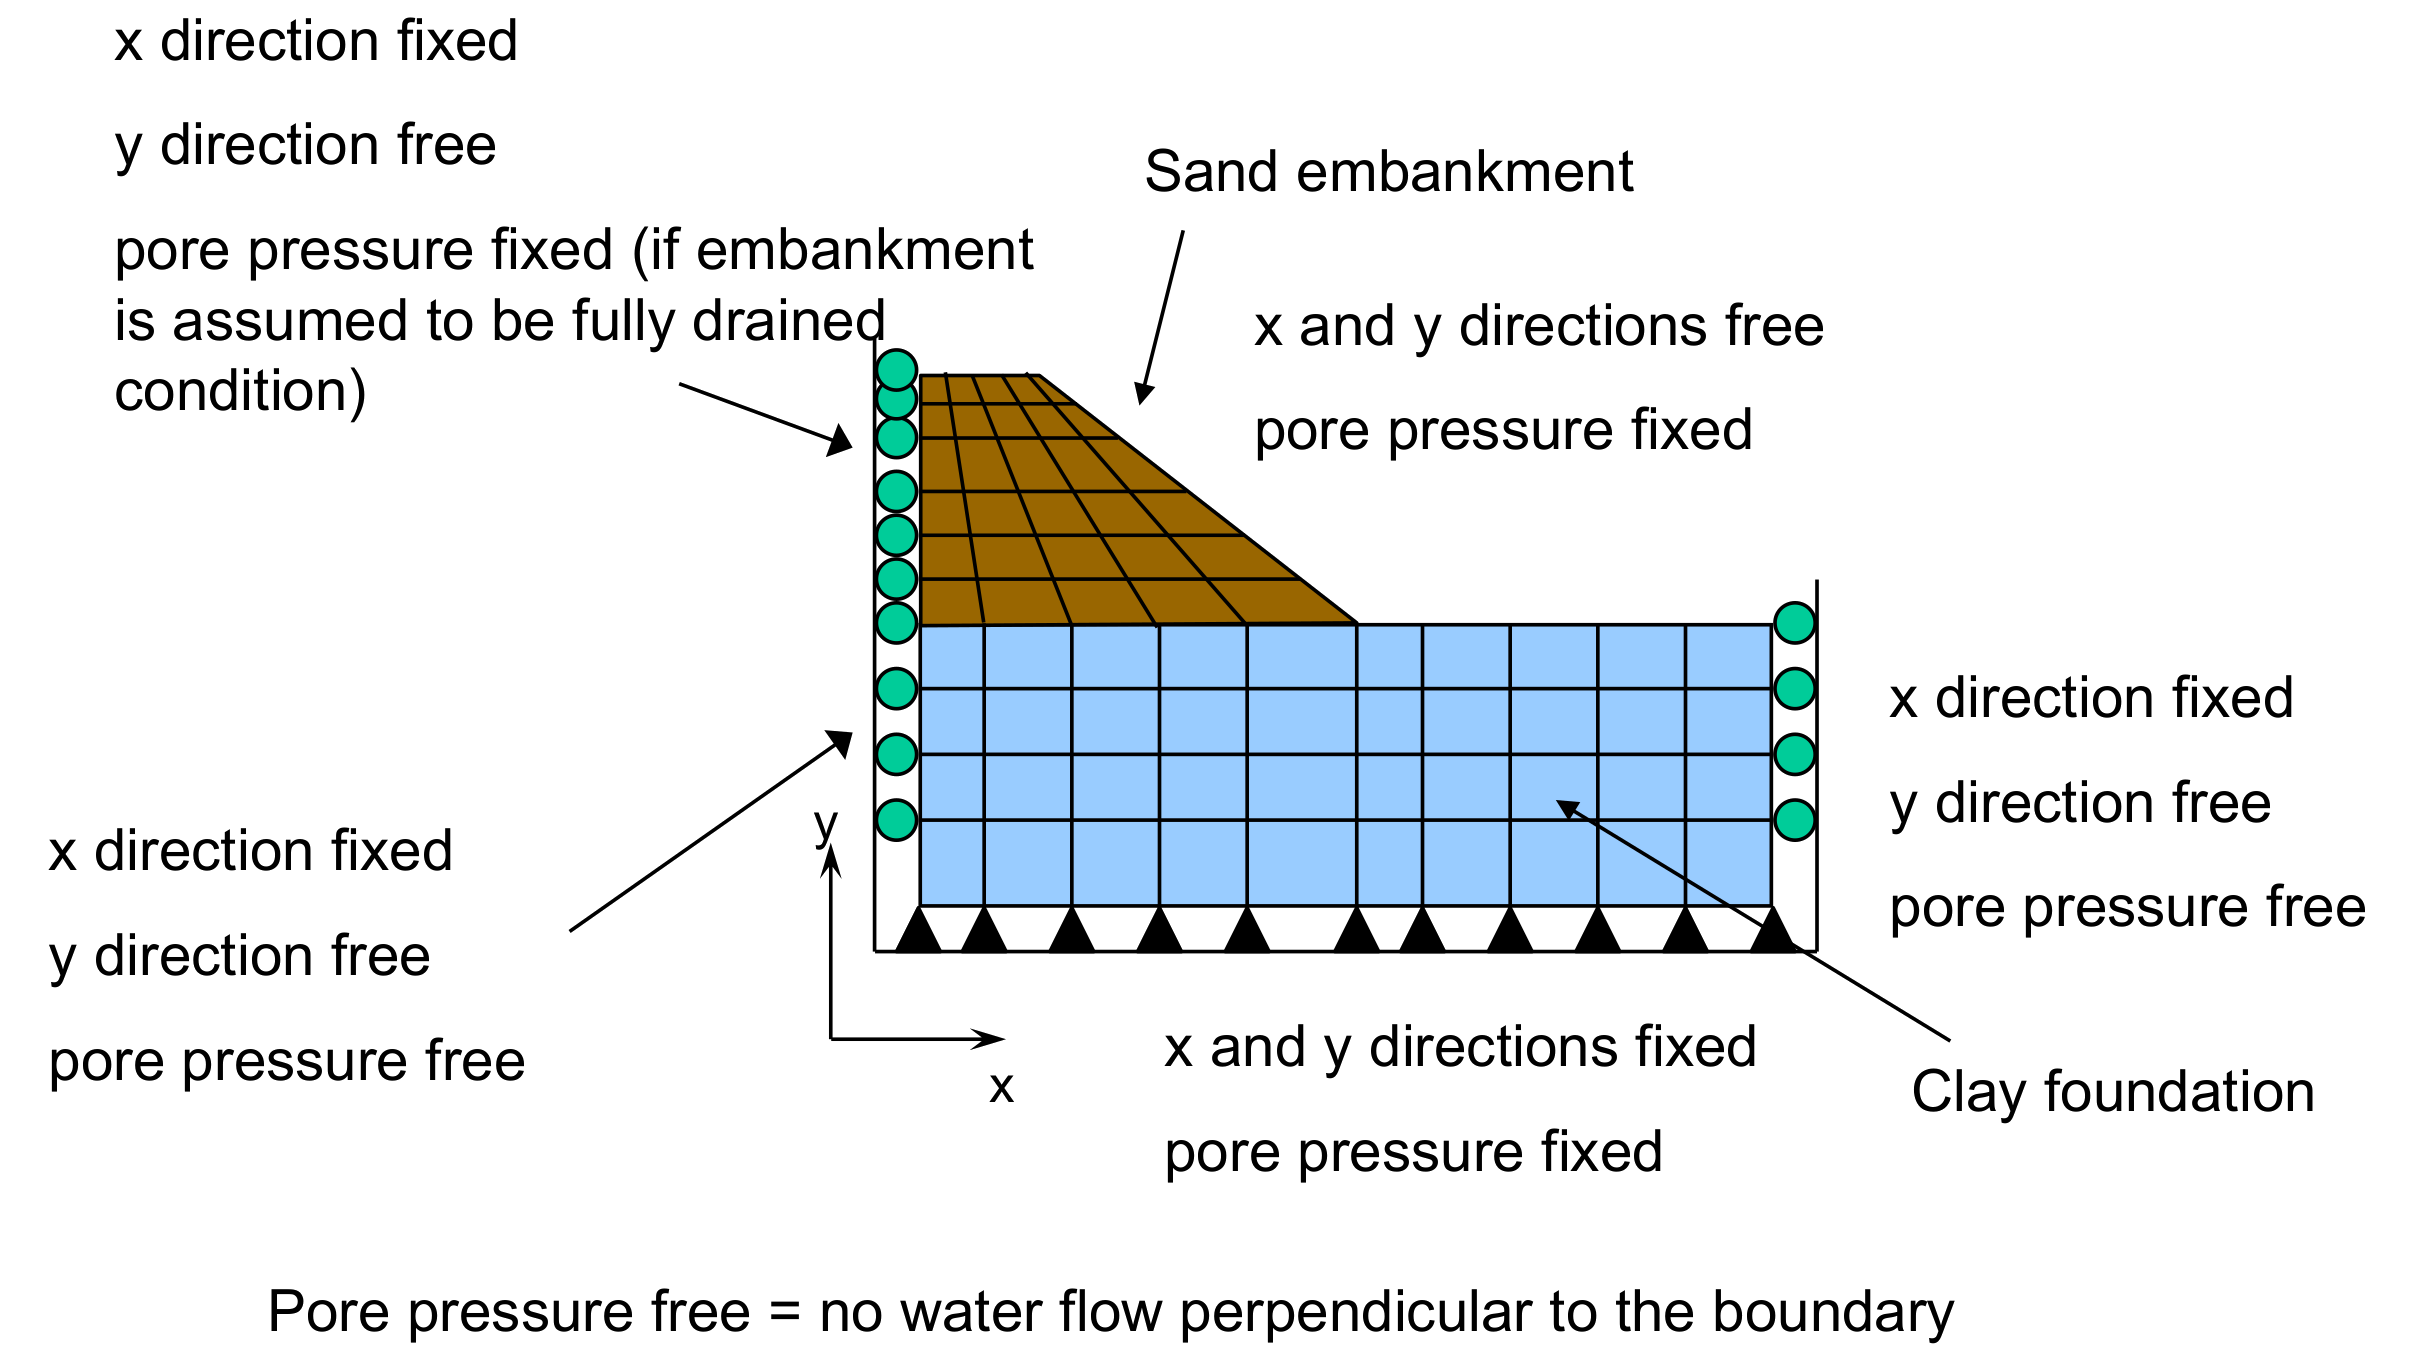
\includegraphics[width=\textwidth]{figs/boundary-conditions.png}
\end{figure}
\end{frame}

%------------------------------------------------
\begin{frame}
\frametitle{FE boundary conditions}
\begin{figure}[ht]
	\centering
	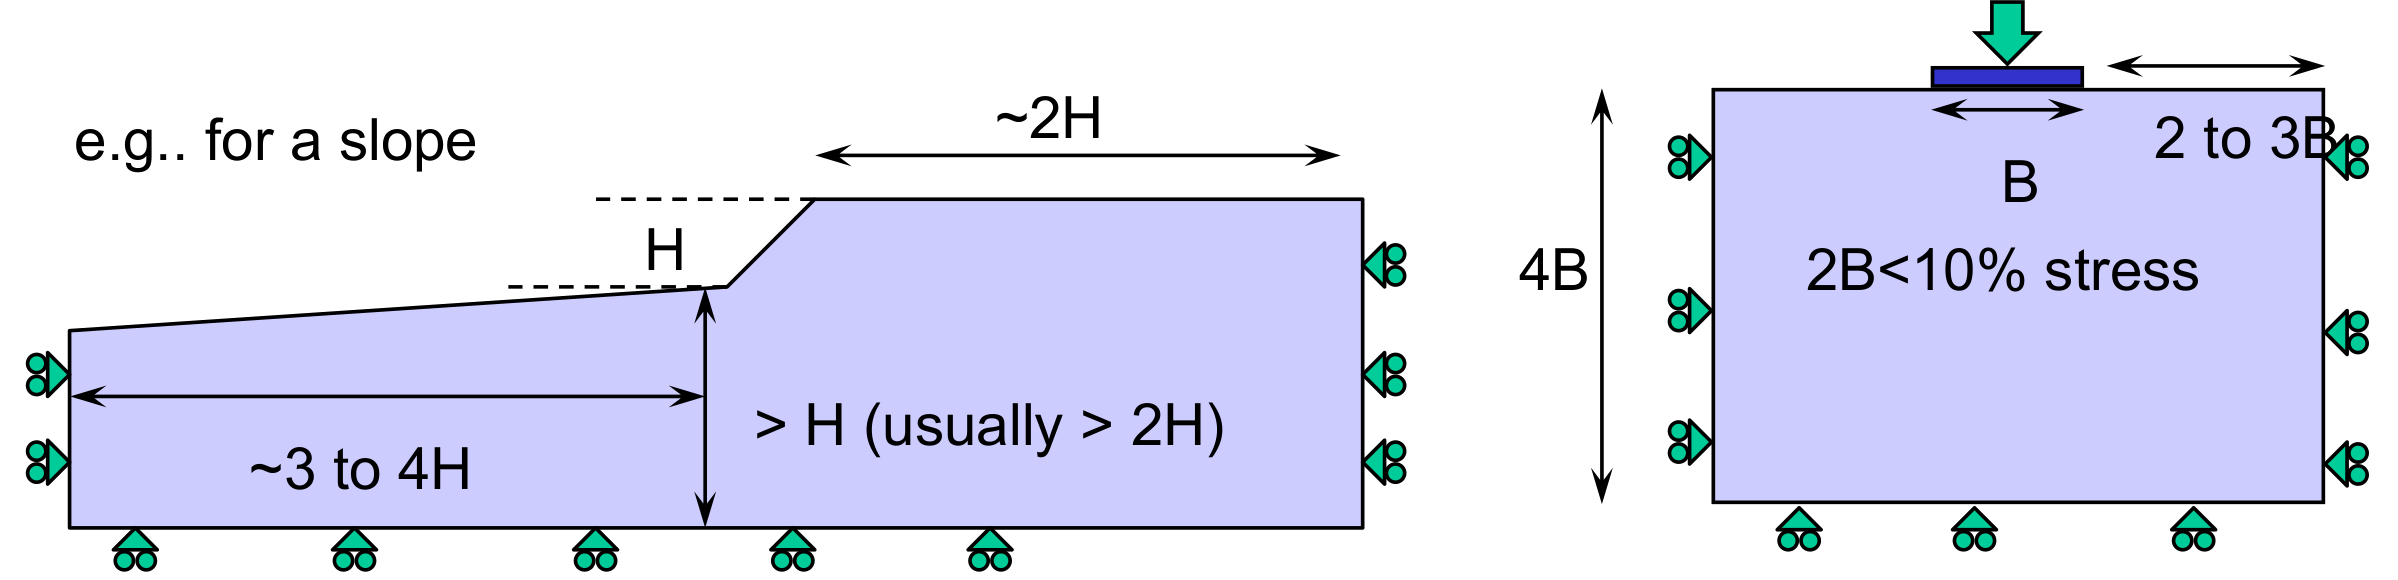
\includegraphics[width=\textwidth]{figs/fe-boundaries.png}
\end{figure}
\end{frame}

%------------------------------------------------
\begin{frame}
\frametitle{FE boundary conditions}
\mode<beamer>{
	\begin{enumerate}
		\item \textbf{Body force}: apply unit weight
		
		\item \textbf{Force}: node is free
		
		\item \textbf{Displacement}: node is fixed
		
		\item \textbf{Pore pressure}: node fixed to apply external pore pressures
	\end{enumerate}
}
\mode<handout>{
	\vspace{3cm}
}

\begin{figure}[ht]
	\centering
	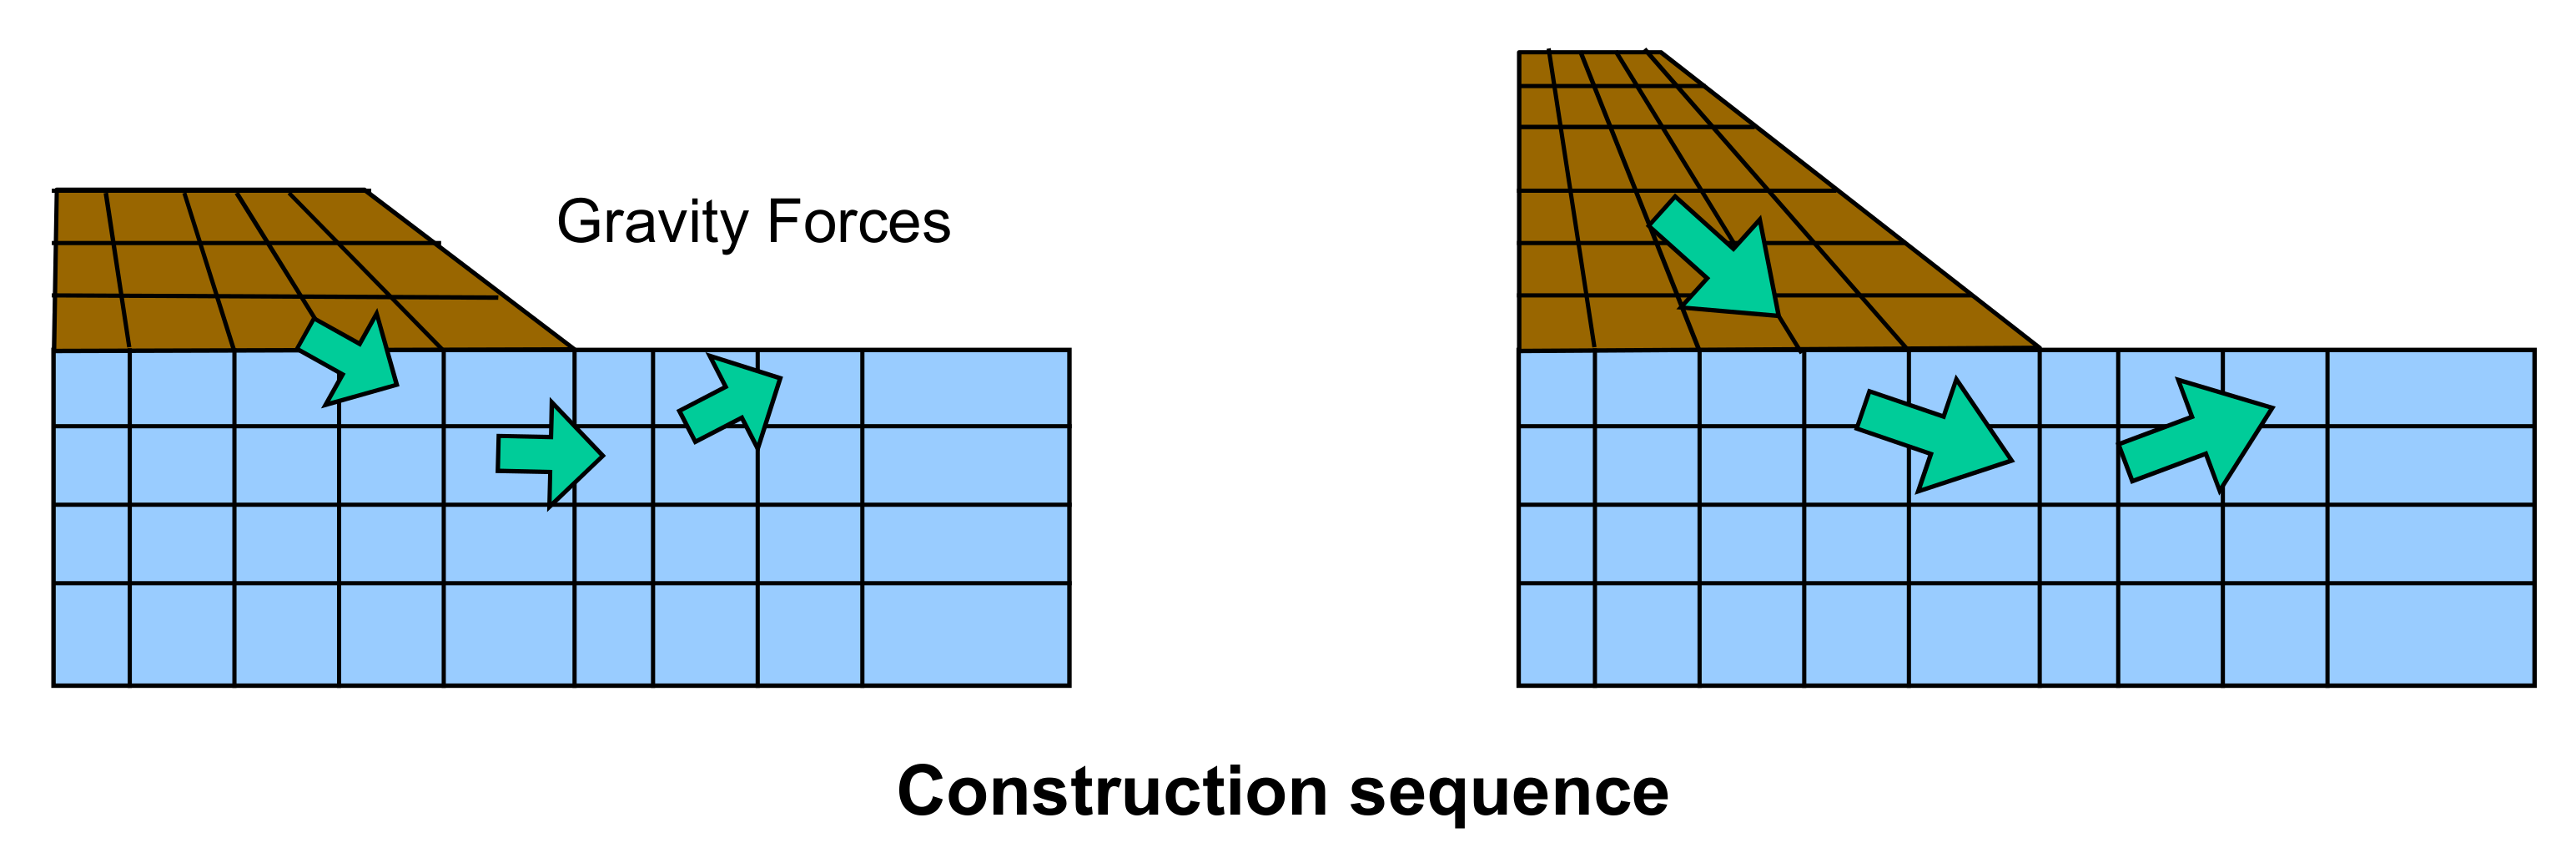
\includegraphics[width=0.75\textwidth]{figs/construction-sequence.png}
\end{figure}
\end{frame}

%------------------------------------------------
\begin{frame}
\frametitle{FE loading conditions}
\begin{figure}[ht]
	\centering
	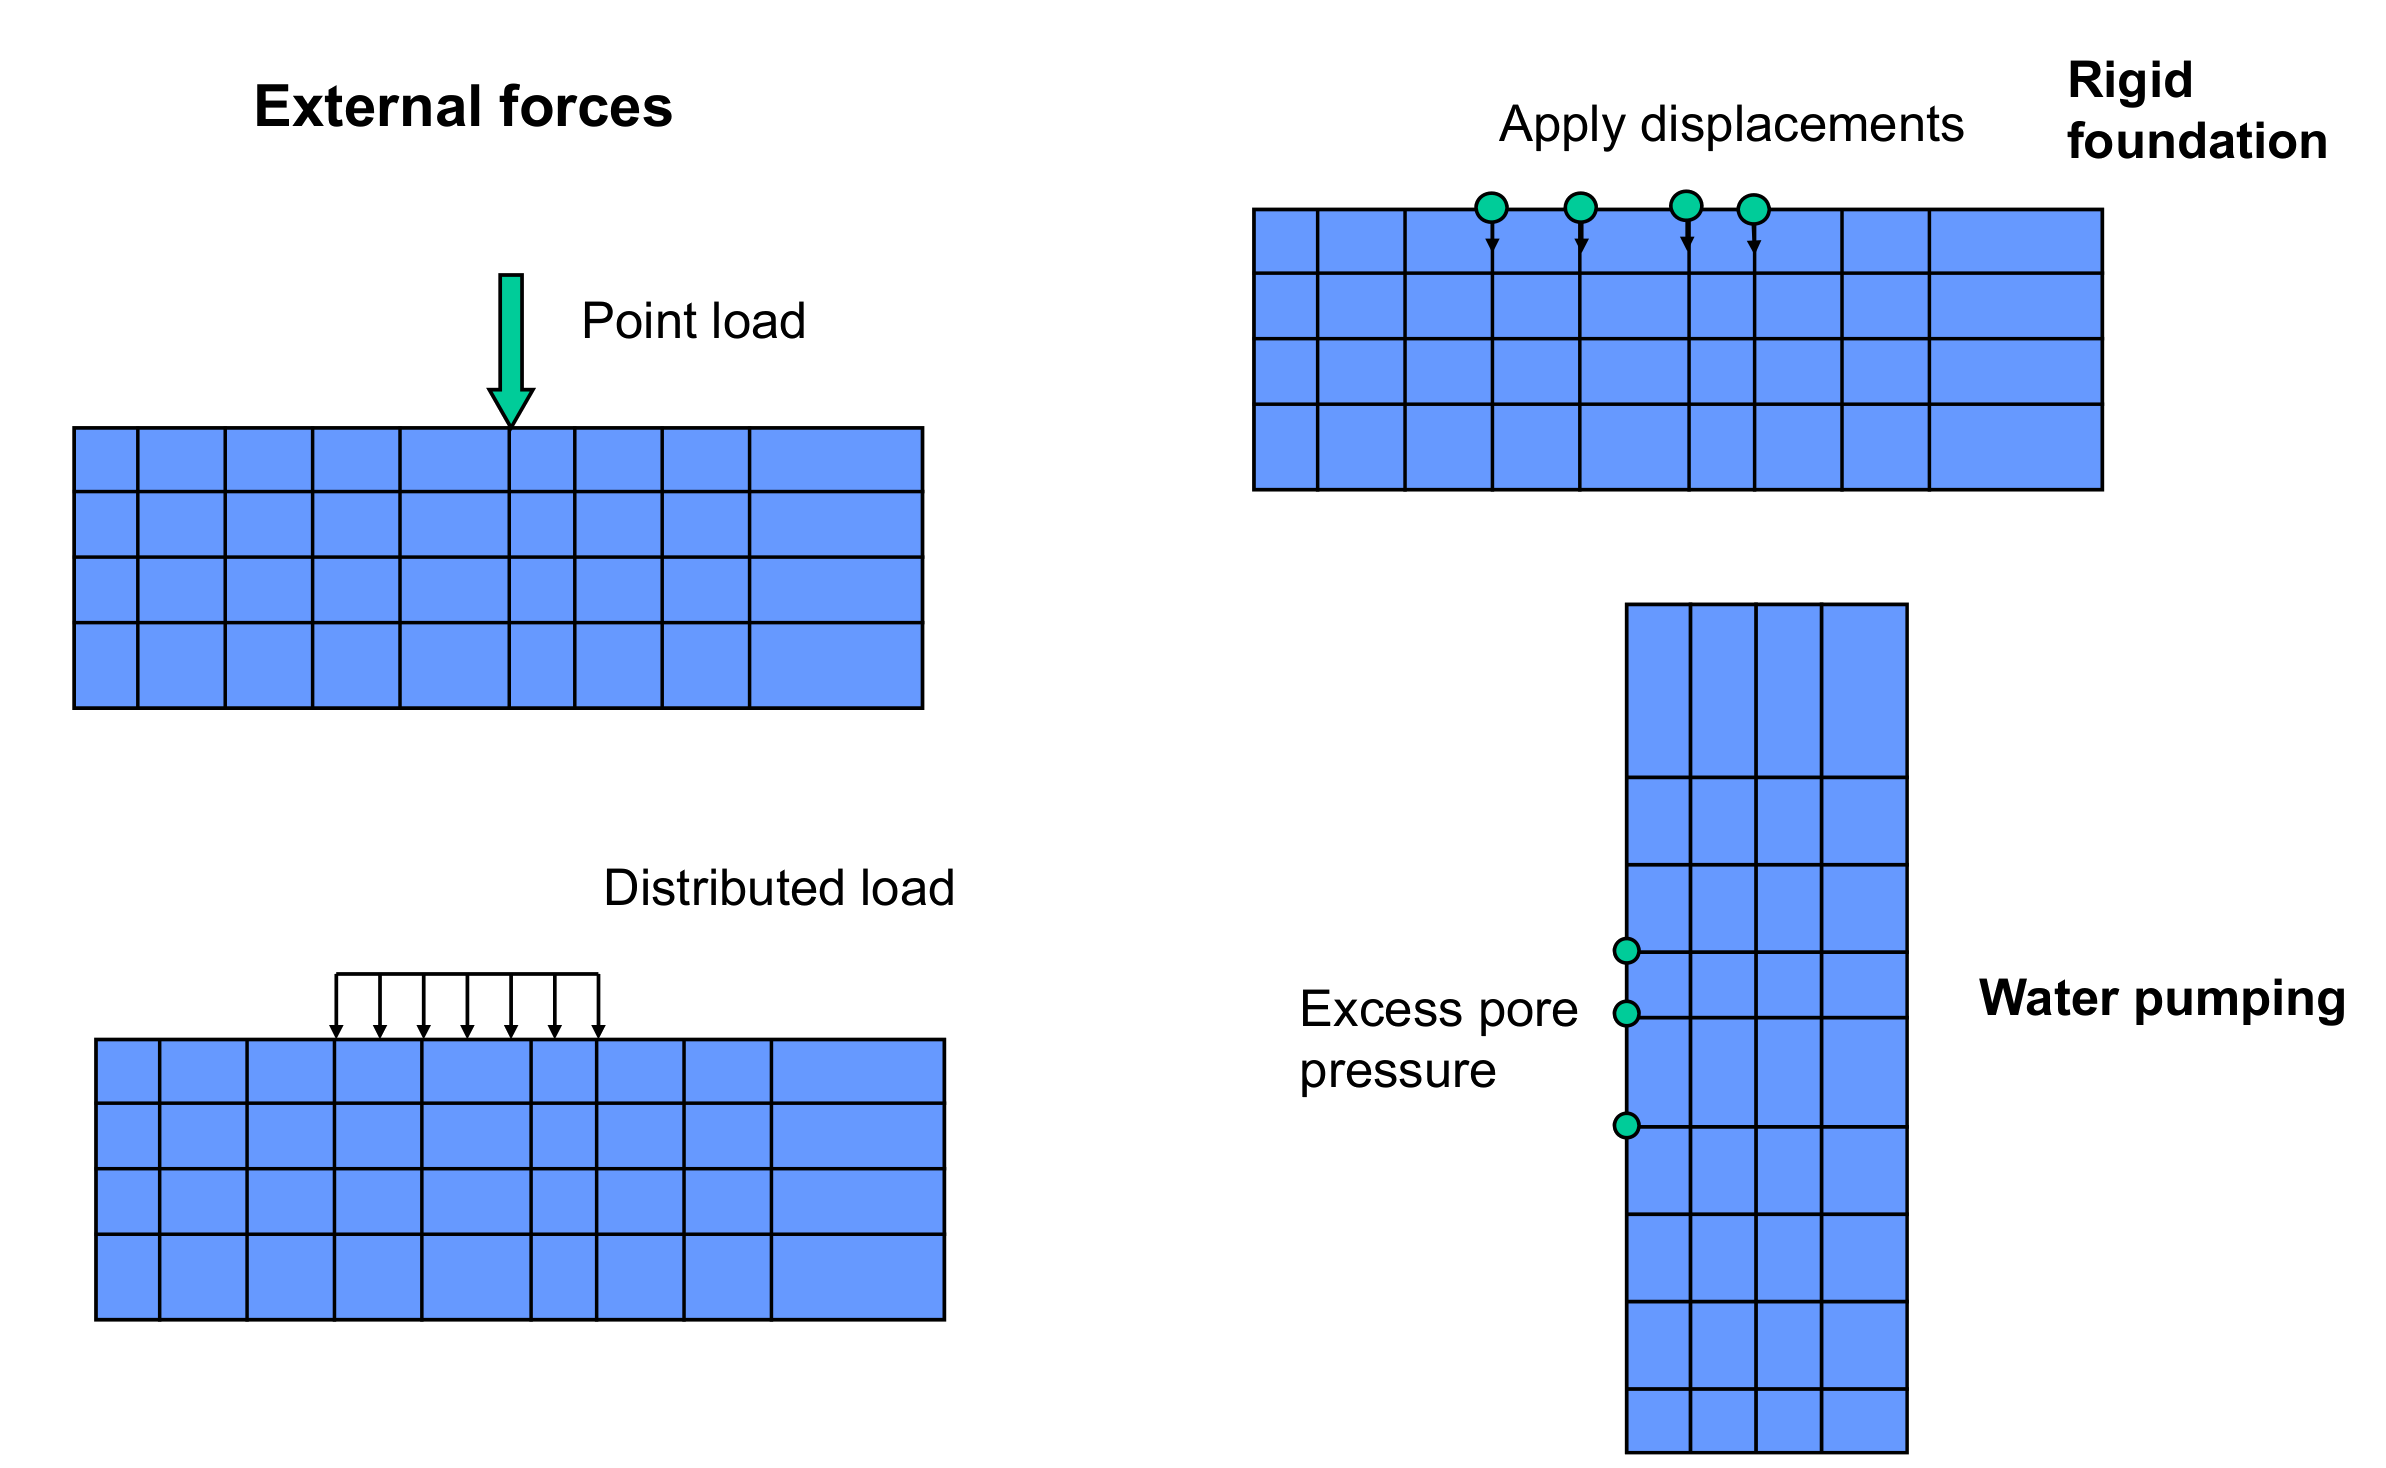
\includegraphics[width=\textwidth]{figs/external-forces.png}
\end{figure}
\end{frame}

%------------------------------------------------
\begin{frame}
\frametitle{FE loading conditions}
\begin{figure}[ht]
	\centering
	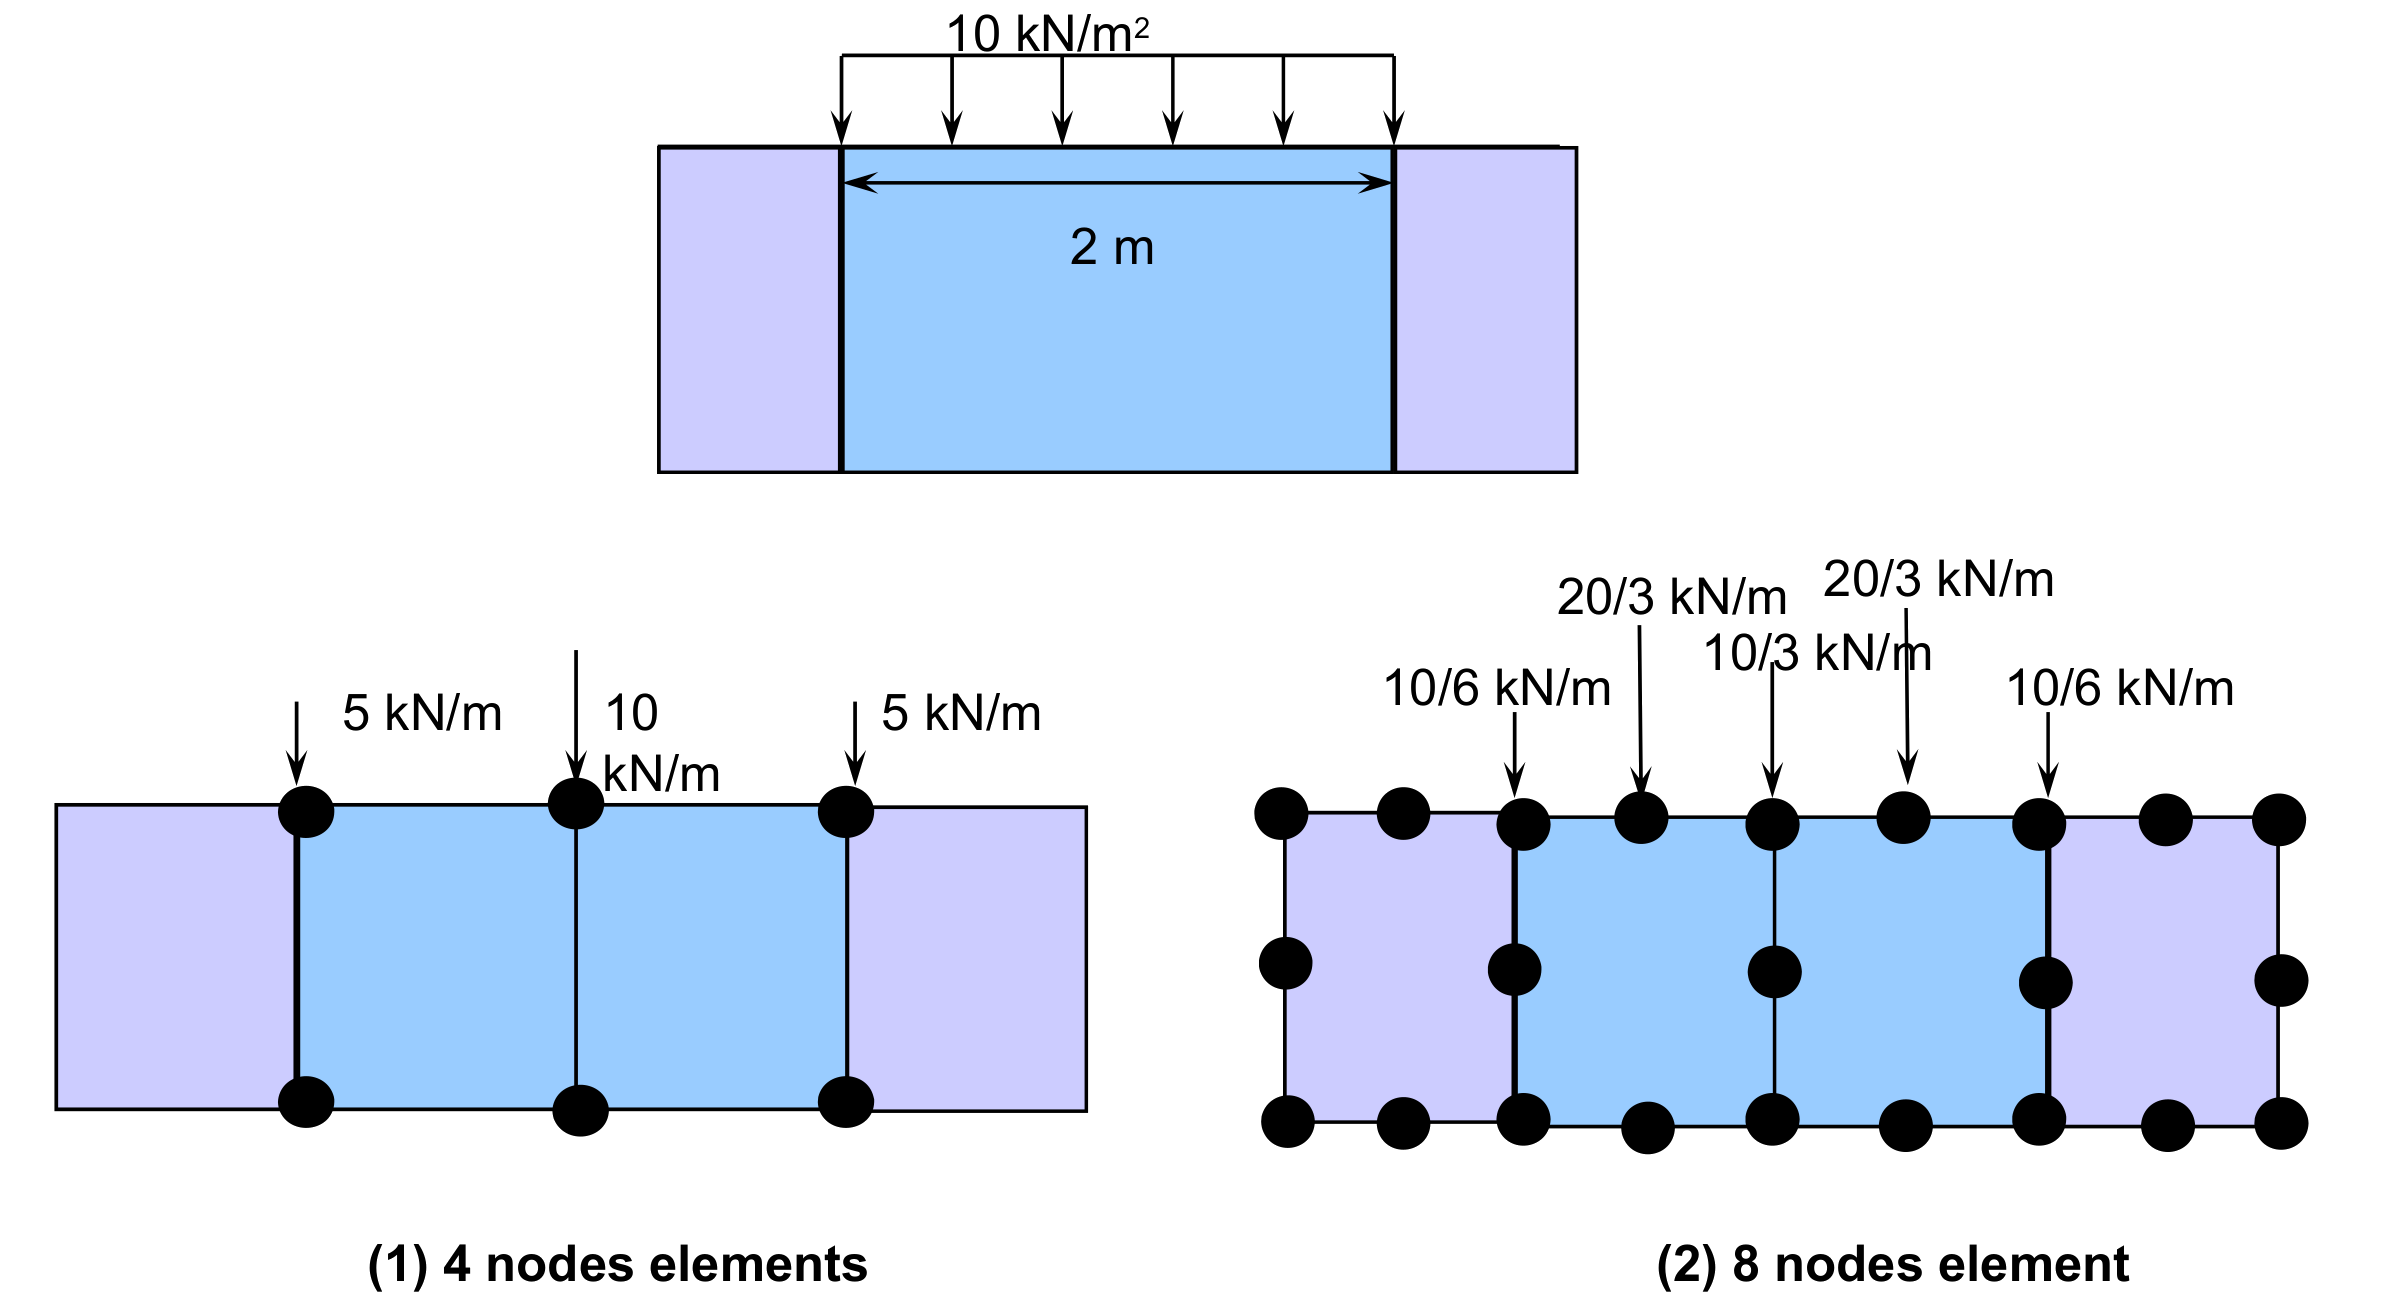
\includegraphics[width=\textwidth]{figs/load-distribution.png}
\end{figure}
\end{frame}

%------------------------------------------------
\begin{frame}
\frametitle{FE stress singularity}

\begin{figure}[ht]
	\centering
	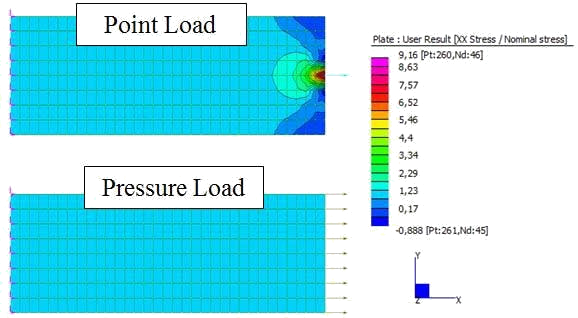
\includegraphics[width=0.75\textwidth]{figs/stress-singularity-load.png}
	\caption*{2D uniaxial bar model. A single point load leads to stress singularities whereas an edge pressure results in a uniform stress field. (Gonzalez., 2015)}
\end{figure}
\end{frame}
\note {
	A stress singularity is a point of the mesh where the stress does not convergence towards a specific value. As we keep refinement the mesh, the stress at this point keeps increasing, and increasing, and increasing... Theoretically, the stress at the singularity is infinite.
	
	Although stress at these singularities is infinite, this does not mean that the model results are incorrect overall. First of all, the displacements are correct even at the singularity point. On the contrary, the stress at the singularity will pollute the stress results near the singularity, however some distance away from the singularity the stress results will be fine! 
	
	As you can see, far away from the point load singularity the stress field is uniform despite of the local singularity. Note that pressure load do not cause point singularities, this is because the pressure attribute is converted by the solver into a set of point loads along the nodes of the edge in a consistent fashion that do not cause a singularity.
}
%------------------------------------------------
\begin{frame}
\frametitle{FE stress singularity}

\begin{figure}[ht]
	\centering
	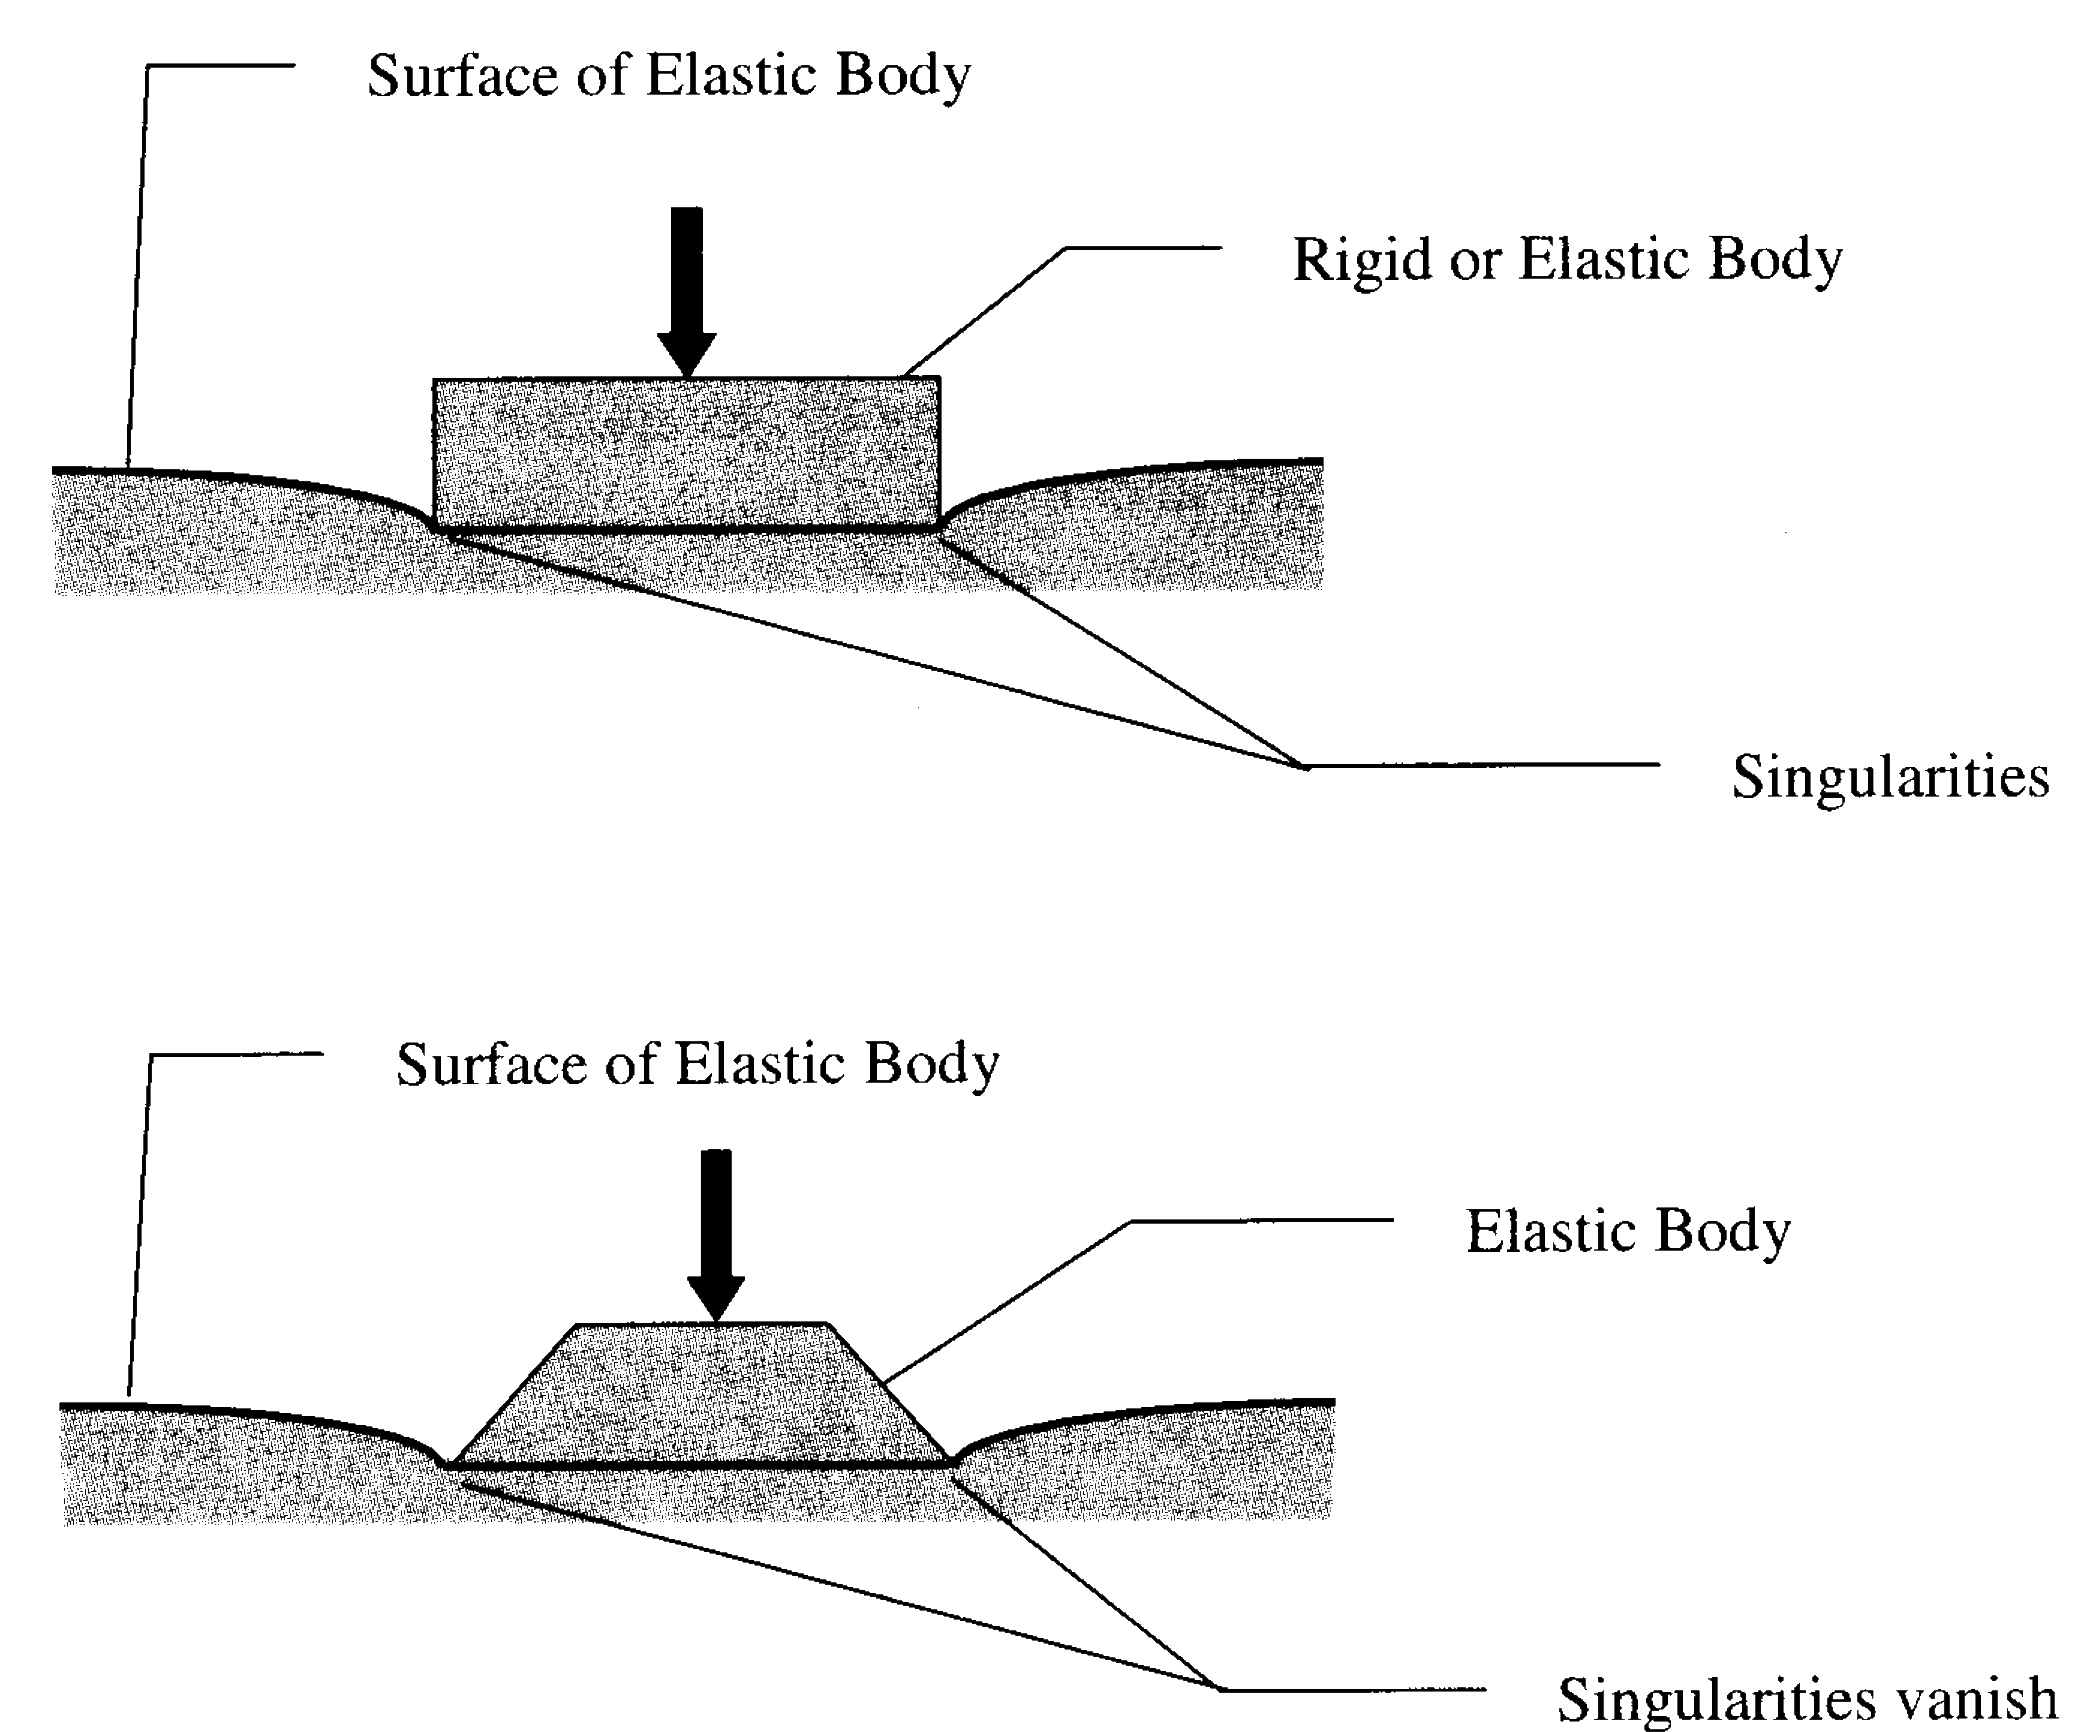
\includegraphics[width=0.75\textwidth]{figs/stress-singularity.png}
\end{figure}
\end{frame}

\note{
	If a concentrated force is applied on a continuum, it results in unbounded stresses, which is called stress
	singularities. The values of stresses become a function of mesh density. The denser the mesh is, the better
	the result becomes. It is often better to replace a concentrated load by a load distributed over a small region
	to avoid the effect of stress singularities.
	
	A sharp re-entrant corner as shown in the figure (a) also produces singularity (i.e. solution is mesh
	dependent and the zones close to the singularity is becomes polluted). The nature of the singularity
	depends on the elastic properties of the two bodies. It may be possible to weaken or eliminate the
	singularity by changing the rectangular object to a tapered one as shown in the figure (b).
}

%------------------------------------------------
\begin{frame}
\frametitle{Geostatic stresses}
Before conducting your analysis, you need to make sure that the stresses in the
ground are the correct values, as the soil behavior depends on the current
in-situ stresses.

\begin{enumerate}
	\item \textbf{list your estimated stresses in the input file}: hopefully the system is in equilibrium
	-- difficult to find the in-situ stresses in the sloping ground.
\end{enumerate}	

\begin{figure}[ht]
	\centering
	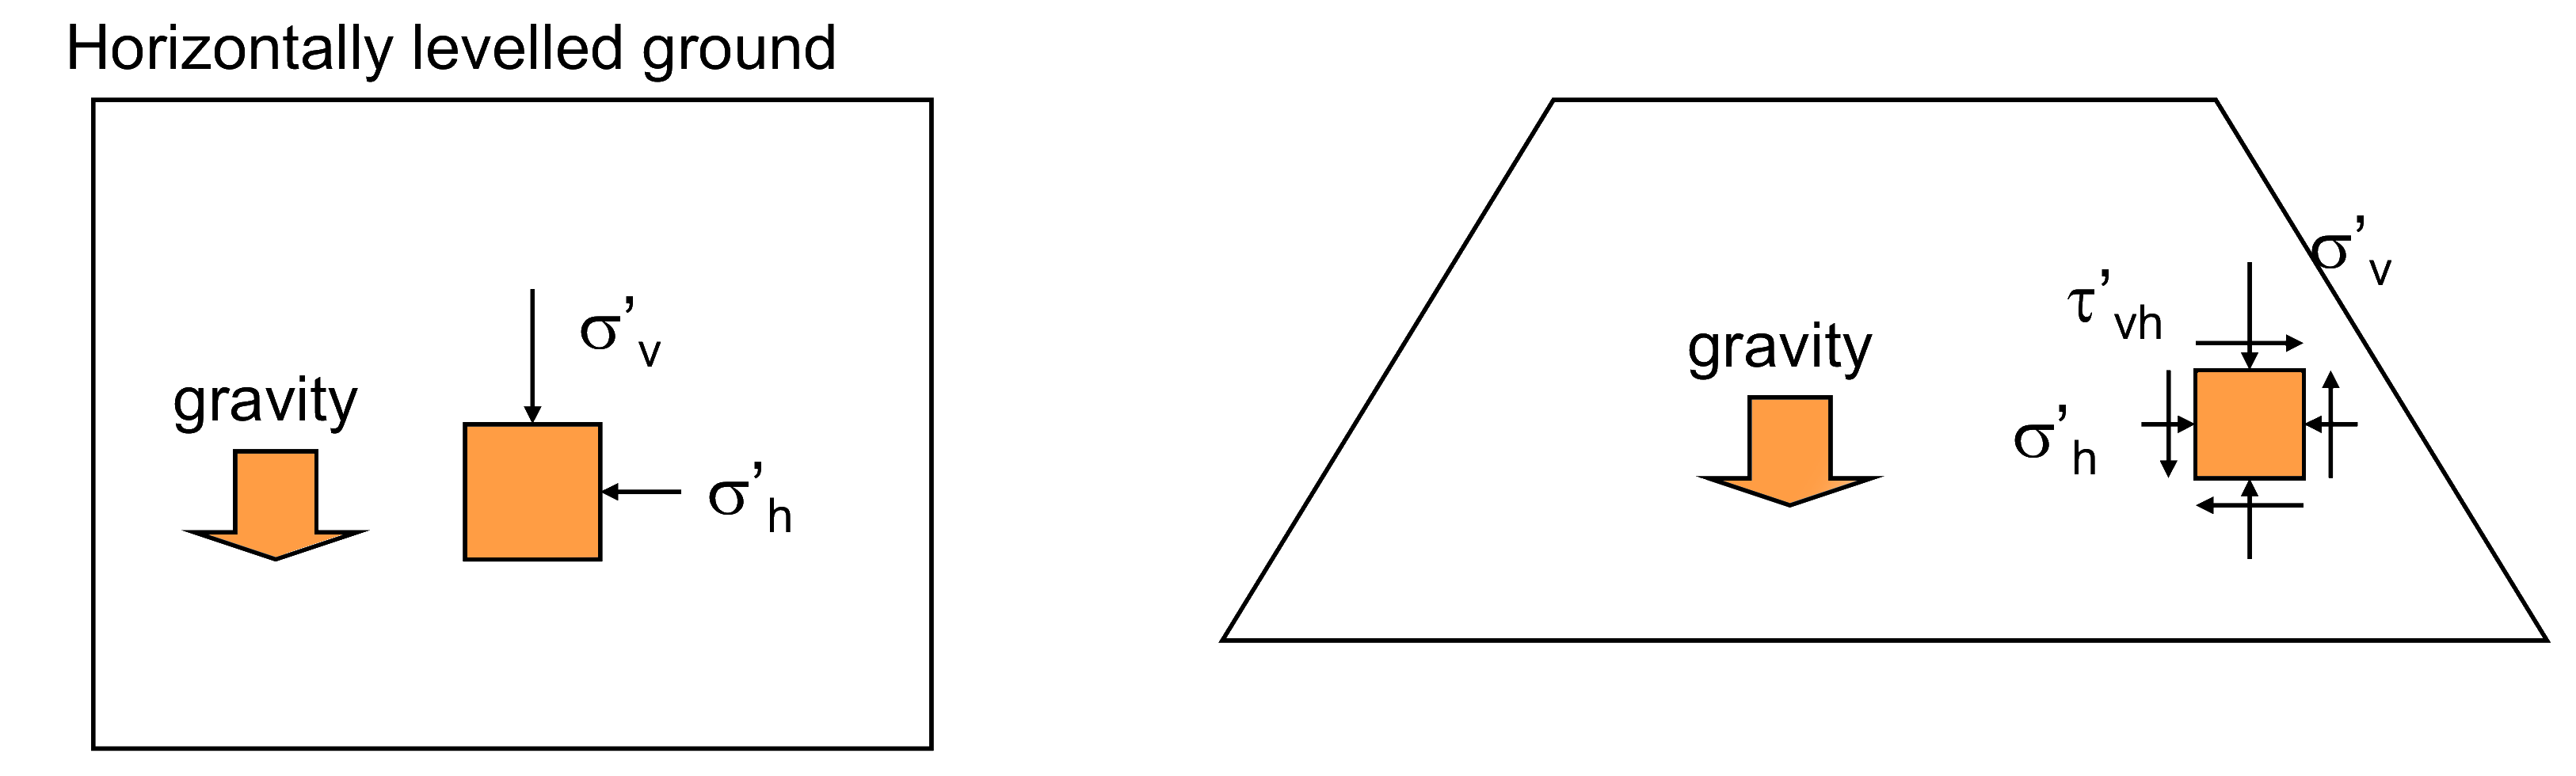
\includegraphics[width=0.75\textwidth]{figs/geostatic-stresses-initial-guess.png}
\end{figure}
\end{frame}

\note{
	\begin{enumerate}
		\item Vertical effective stress $\sigma_v^\prime$ from the unit weight of the soil
		\item Horizontal effective stress $\sigma_h^\prime = K_0 \sigma_v^\prime$ 
		\item Estimation of in-situ stresses becomes difficult - depends on soil model used.
		\item \textbf{Total stress analysis – need to give initial total stresses}
	\end{enumerate}
}

%------------------------------------------------
\begin{frame}
\frametitle{Geostatic stresses}
\begin{enumerate}
	\setcounter{enumi}{1}
	\item \textbf{Zero displacement approach} - ask the program to compute the in-situ stresses
		from the equilibrium condition (very few programs allow you to do this)
		\begin{figure}[ht]
			\centering
			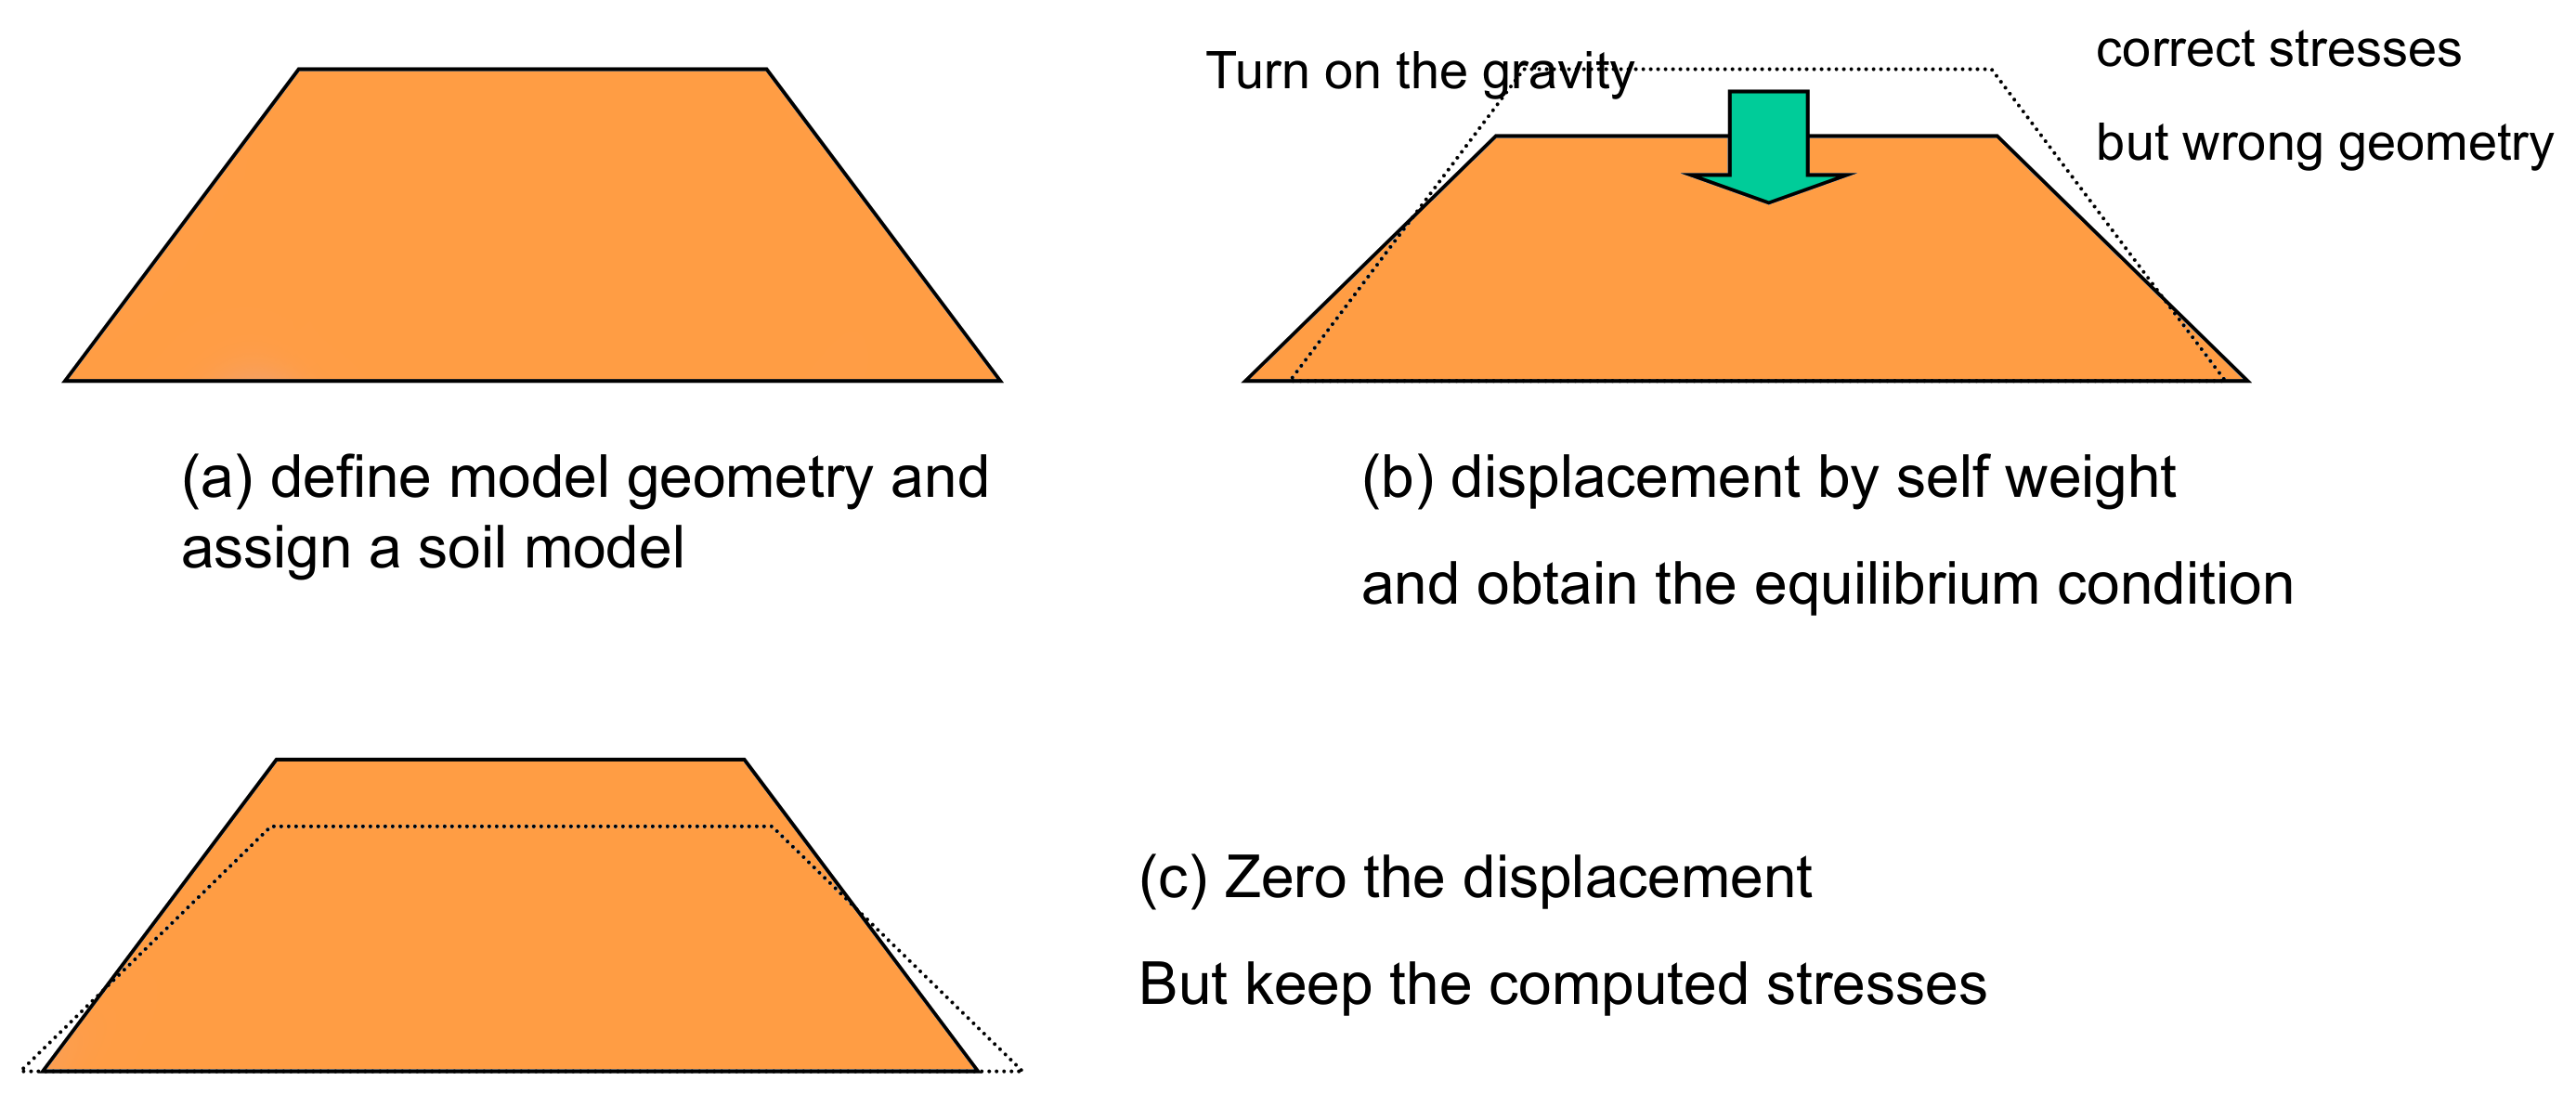
\includegraphics[width=0.75\textwidth]{figs/geostatic-stresses-zero-disp.png}
		\end{figure}
	\item \textbf{Intermediate approach} - Guess the insitu stress distribution, apply gravity and
	perform the equilibrium check (hopefully the displacements are zero) - ABAQUS
	GEOSTATIC approach
\end{enumerate}	
\end{frame}

%------------------------------------------------
\begin{frame}
\frametitle{The coefficient of earth pressure at rest $K_0$}
	\begin{itemize}
		\item \textbf{Normally consolidated soils}
	\mode<beamer>{
		\begin{itemize}
			\item 	Cam-clay predictions (Wood, 1990).
			$K_0$ (Modified CC) $< K_0$ (Original CC)
			\item 	$K_0 = K_{\mathrm{nc}} = 1 - \sin \phi^\prime$ (Jaky, 1944) ($\phi^\prime$ is the friction angle of the soil).
		\end{itemize}
	
	}
	\mode<handout>{
		\vspace{3cm}
	}
	\item \textbf{Over consolidated soils}
		\begin{itemize}
			\item \textbf{Cam-clay predictions}
			$K_{\mathrm{oc}} = (1 - \sin \phi^\prime) \times \mathrm{(OCR)}$  (Mayne et al., 1982)
			up to $K_p = (1 + \sin  \phi^\prime)/(1 - \sin  \phi^\prime)$
			
			\item \textbf{Wroth's method (1975)}
			$K_{\mathrm{oc}} = \mathrm{(OCR)} K_{\mathrm{nc}} - \left(\frac{\nu^\prime}{1 - \nu^\prime}\right) (\mathrm{OCR} -1)$ for OCR $< 5$ and $\nu^\prime$ is the poisson’s ratio = 0.254 - 0.371.
		\end{itemize} 
	\end{itemize}
\end{frame}

%------------------------------------------------
\begin{frame}
\frametitle{Soil models}
\begin{figure}[ht]
	\centering
	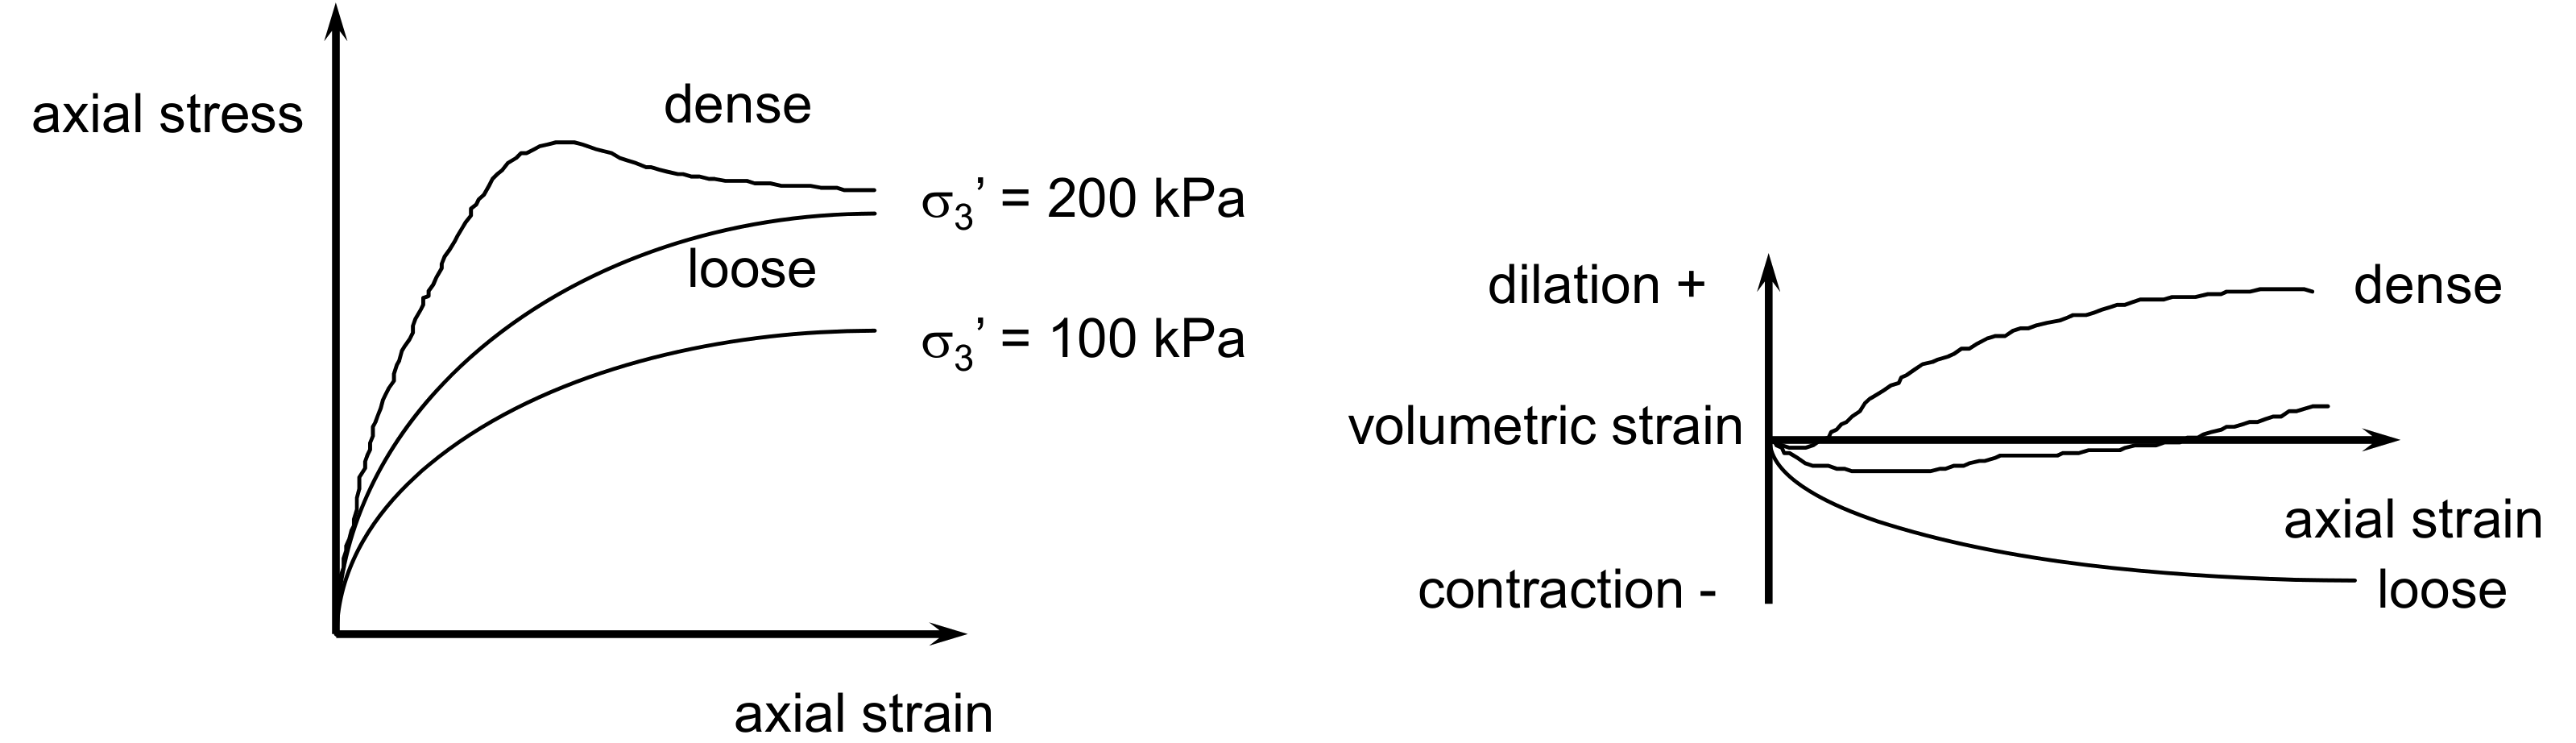
\includegraphics[width=0.9\textwidth]{figs/soil-models.png}
\end{figure}
\mode<beamer>{
	\begin{enumerate}
		\item \textbf{Sand} - Linear elastic model, Non-liner elastic model, Drucker-Prager elasto-plastic model,
		Mohr-coulomb elasto-plastic model or Advanced models ?
		\item \textbf{Clay} - Linear elastic model, Non-linear elastic model, Cam-clay model, or Advanced models ?
	\end{enumerate}
}
\mode<handout>{
	\vspace{2cm}
}
\end{frame}

%------------------------------------------------
\begin{frame}
\frametitle{Verification of Design Parameters (Atkinson., 1995)}
\mode<beamer>{
	\begin{enumerate}
		\item Are the soil models and analyses being used appropriate for the
		soils and for the structure?
		\item Are the design parameters being measured appropriate for the
		soil models being used?
		\item Are the tests being carried out the appropriate ones to determine
		the required design parameters?
		\item Is the laboratory where the tests are being done capable of doing
		the required tests? Ideally, the engineer should inspect the
		laboratory and equipment, observe tests and check the
		procedures being used to analyse and interpret the results.
		\item Are the correct samples being used? Are the appropriate methods
		of sample preparation being used? Do you need high quality
		samples or reconstituted samples?
	\end{enumerate}
}
\end{frame}

%------------------------------------------------
\begin{frame}
\frametitle{Verification of Design Parameters (Atkinson., 1995)}
\mode<beamer>{
	\begin{enumerate}
		\item Have any tests been done which investigate whether the soils
		reasonably follow the critical state theories or the elasto-plastic
		theories being used in the analyses?
		\item Have tests being carried out at stress levels corresponding to
		the range of stresses in the ground? Is it necessary to follow
		special stress paths representing the previous stress history and
		the current loading?
		\item Have linear parameters been fitted to non-linear test results over
		appropriate ranges?
		\item Are the design parameters internally self consistent? Do
		parameters determined from triaxial or other loading tests
		correspond to parameters estimated form the grading and
		nature of the grains? How the values compare to the values
		obtained from empirical equations?
	\end{enumerate}
}
\end{frame}


\subsection{Errors in FEA}
%------------------------------------------------
\begin{frame}
\frametitle{FE errors}
\mode<beamer>{
	\begin{figure}[ht]
		\centering
		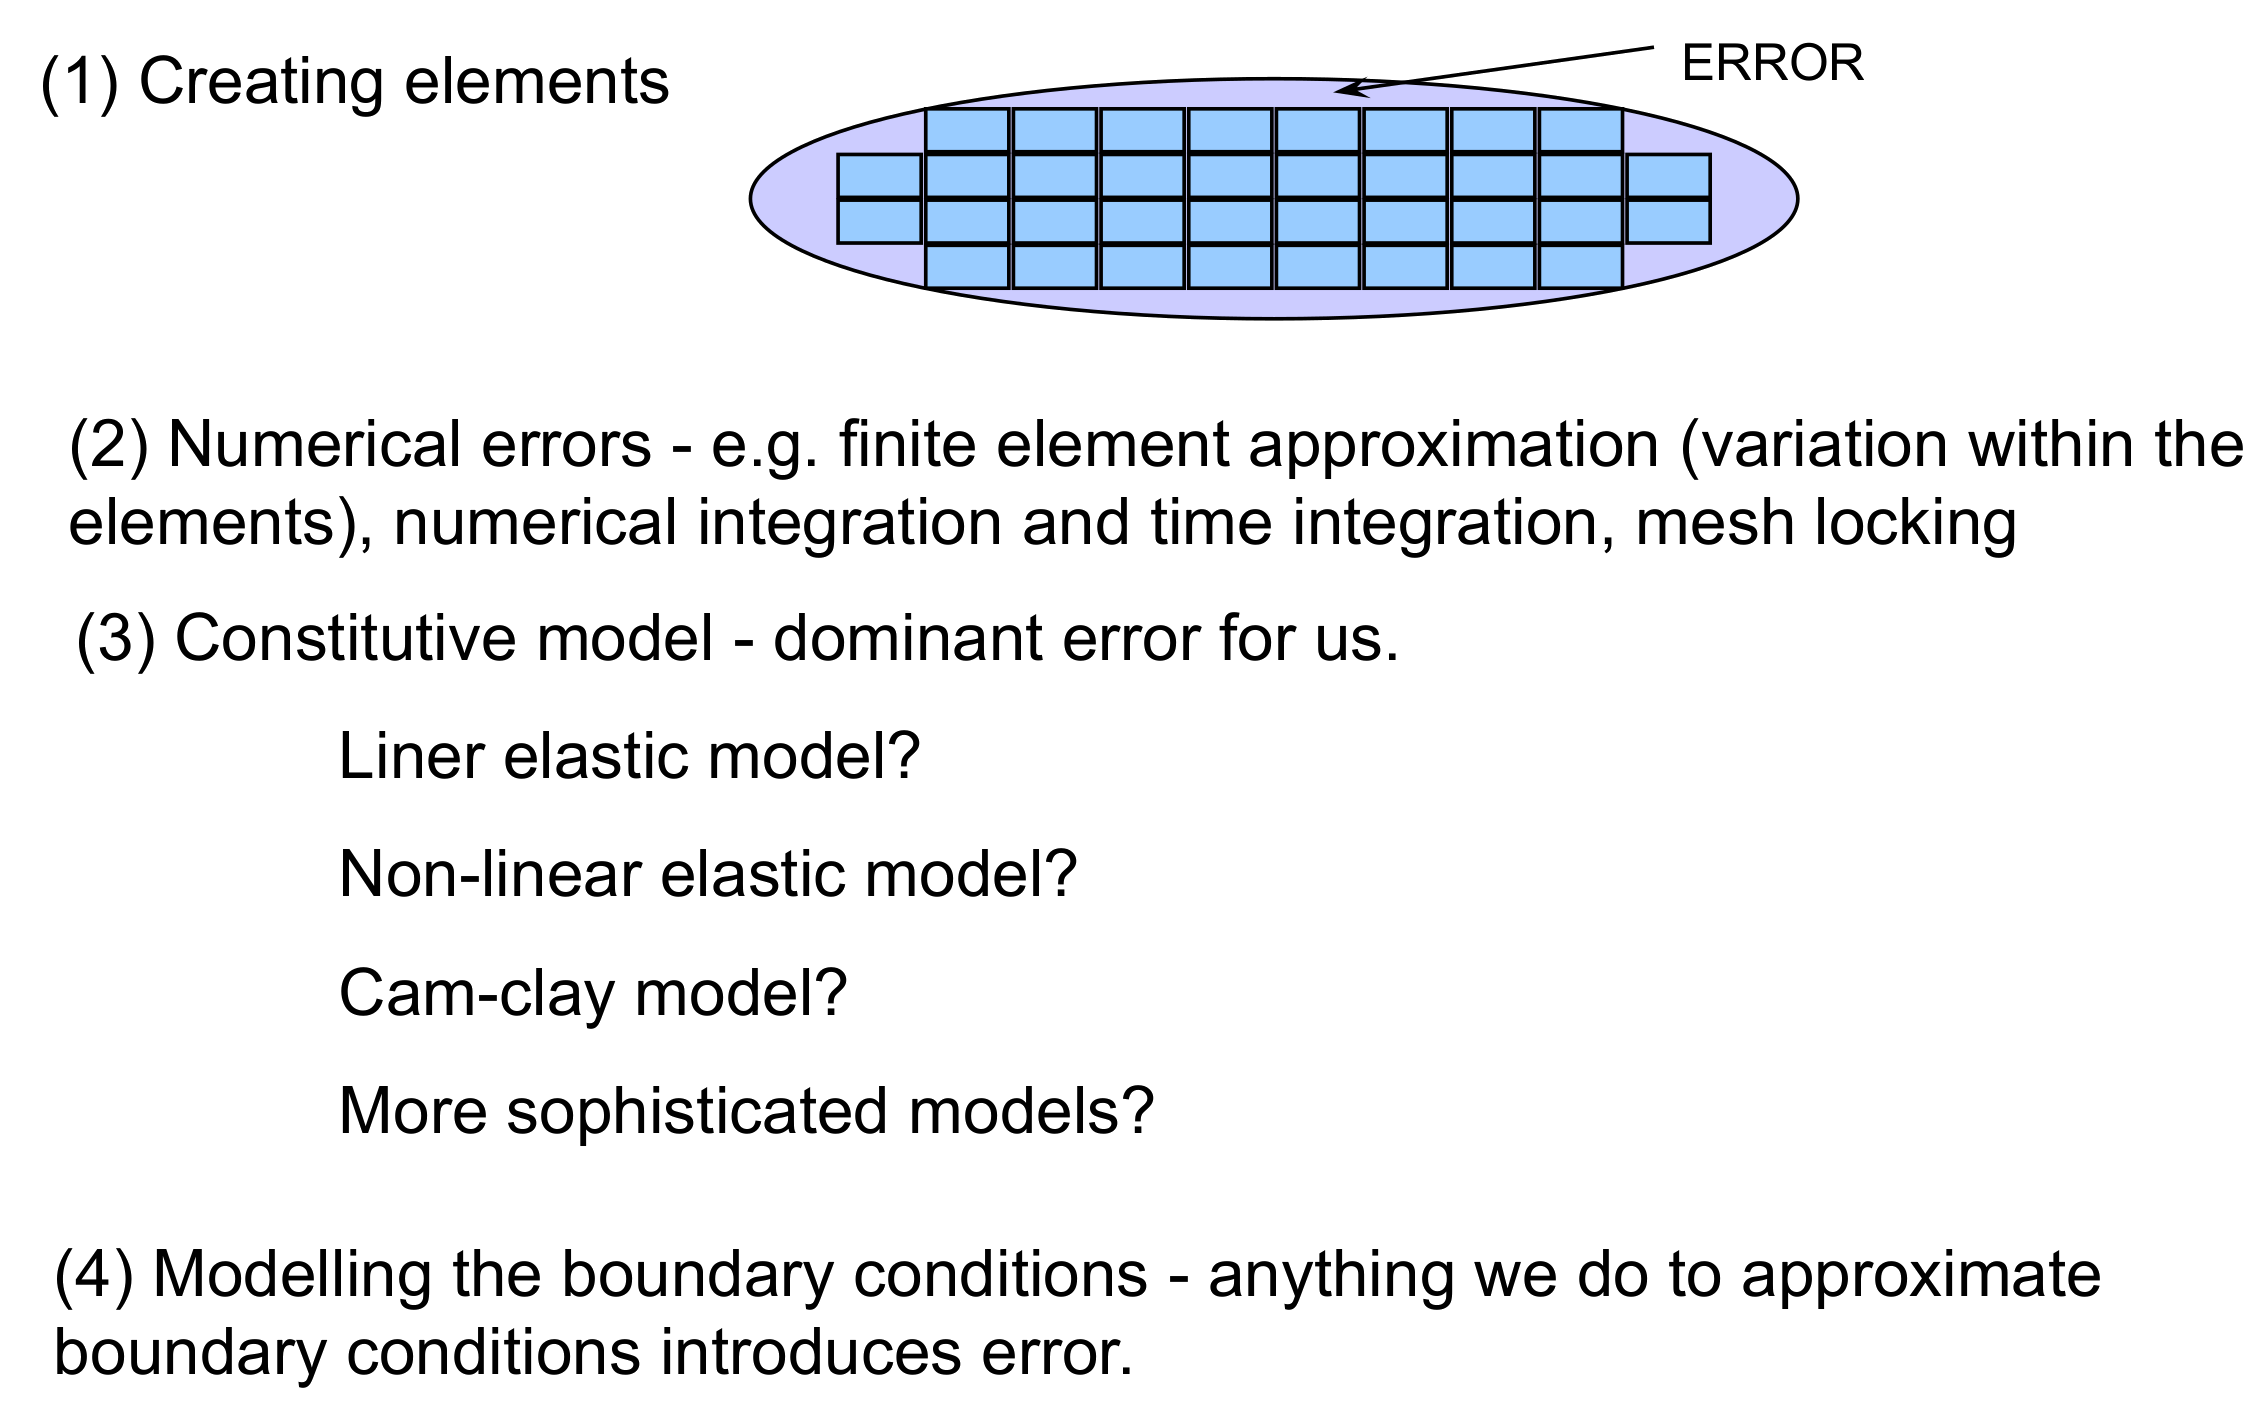
\includegraphics[width=0.9\textwidth]{figs/fe-errors.png}
	\end{figure}
}
\mode<handout>{
	\vspace{6cm}
}
\end{frame}

%------------------------------------------------
\begin{frame}
\frametitle{Check! Check! Check!}
\mode<beamer>{
	\begin{itemize}
		\item Use well documented field study or model study
		\item Do hand calculations or use chart solution
		\item Check orientations of the maximum principal stress directions - tells
		how loads flowing through the system
		\item Check failure parameters-how close to failure line, look to see whether
		reasonable
		\item check the vertical stress $\sigma_v$ and $\sigma_h$.
	\end{itemize}
}
\mode<handout>{
	\vspace{4cm}
}
\begin{figure}[ht]
	\centering
	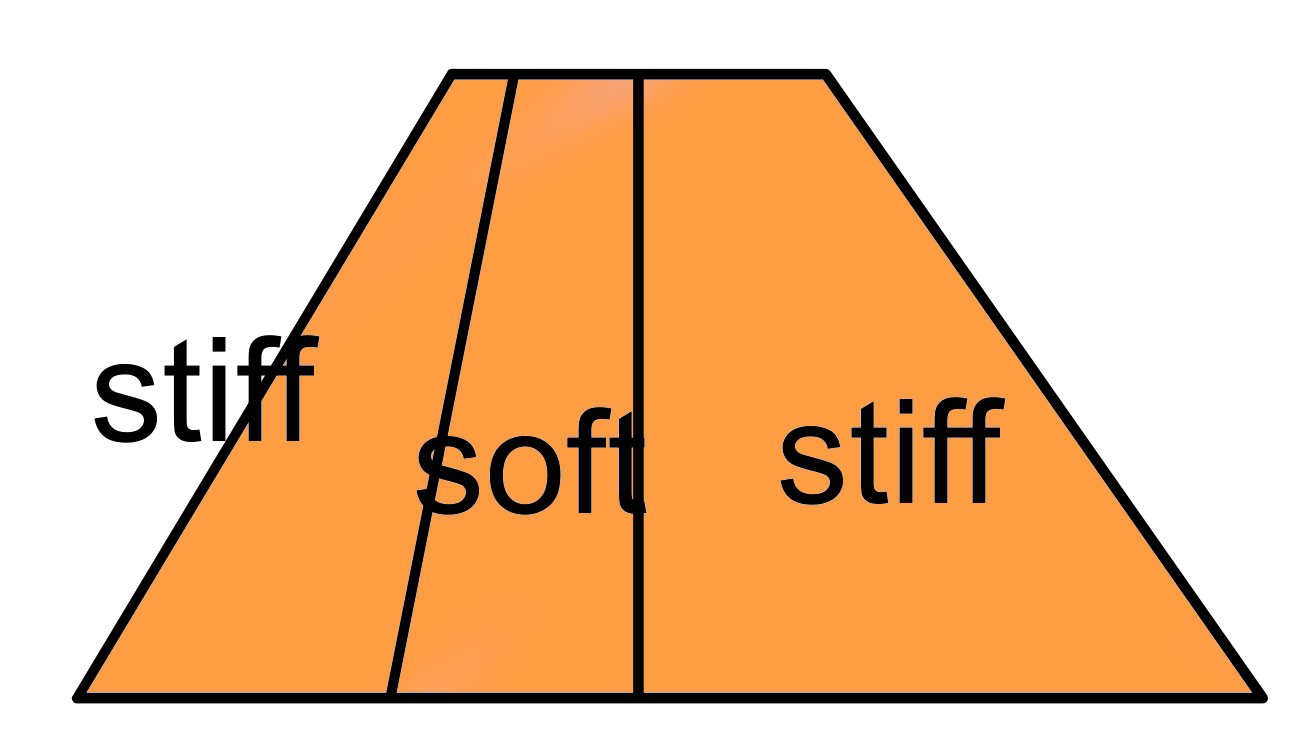
\includegraphics[width=0.3\textwidth]{figs/vertical-stresses.png}
	\caption*{Beware : $\sigma_v$ here lower than $\gamma h$ due to stress transfer to stiff material - hanging up}
\end{figure}
\end{frame}

%------------------------------------------------
\begin{frame}
\frametitle{Pore-pressure analysis in geotechnical engineering}
\mode<beamer>{
	\begin{figure}[ht]
		\centering
		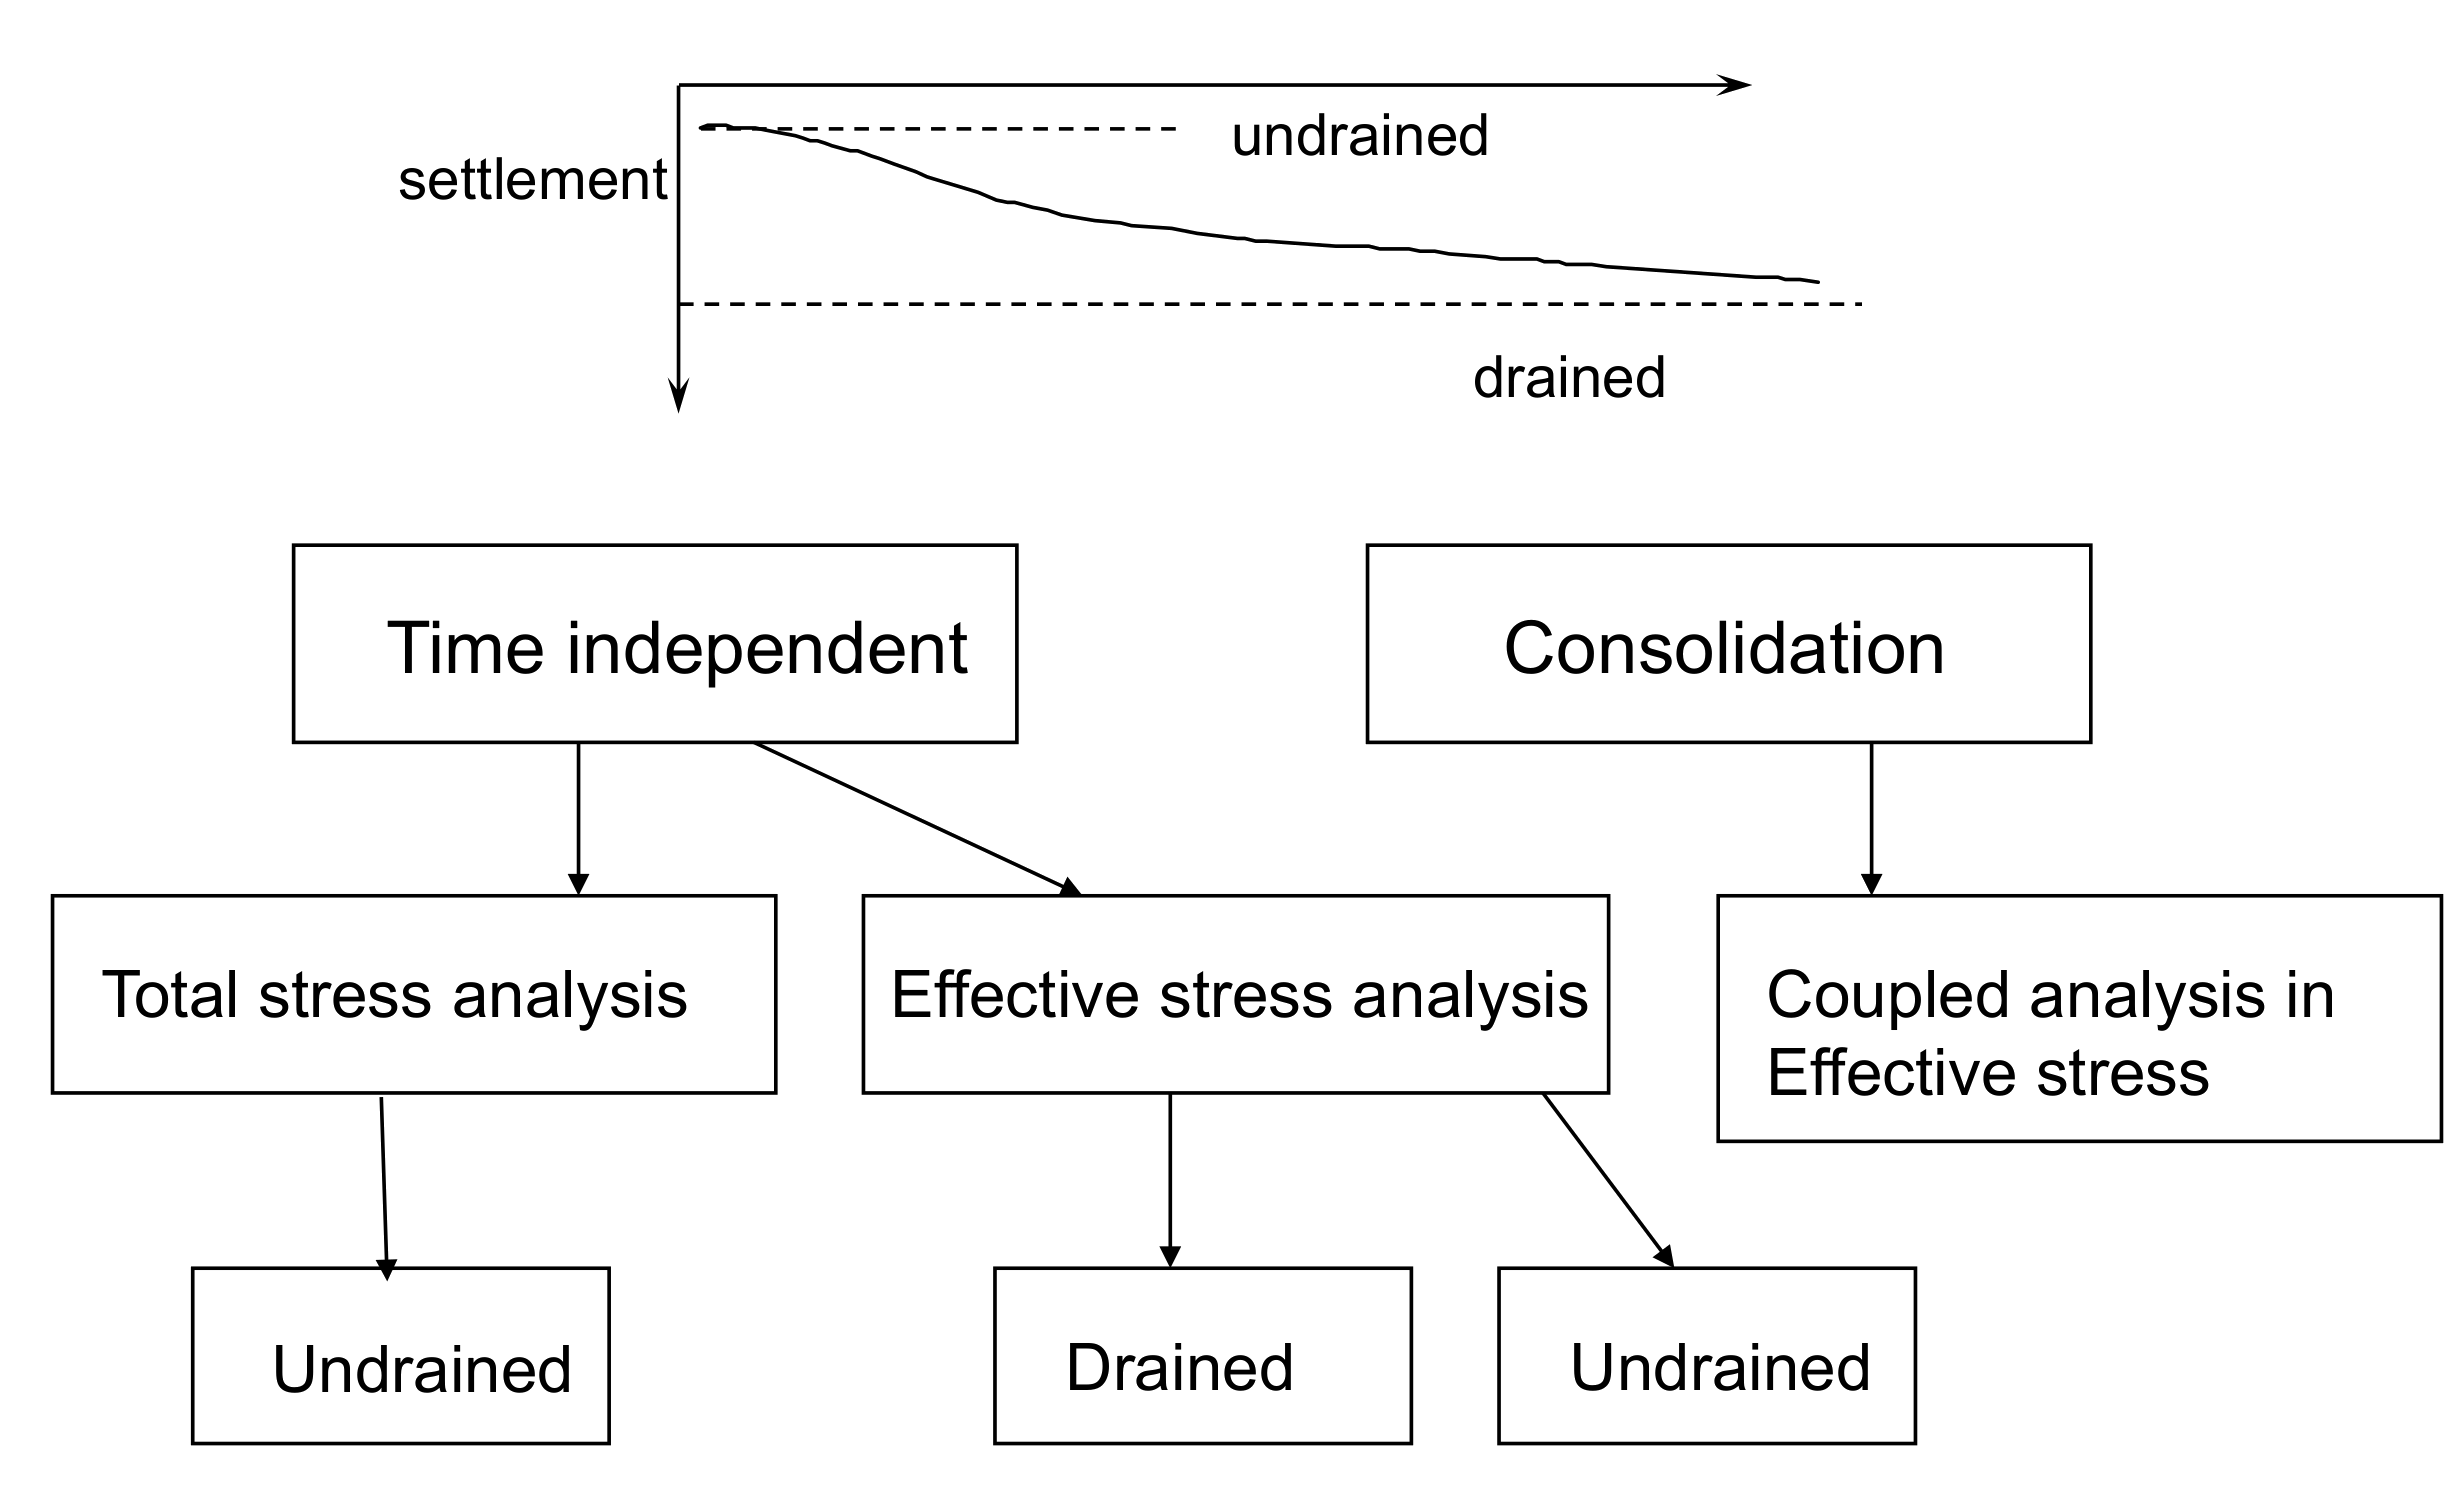
\includegraphics[width=\textwidth]{figs/geotechnical-analysis.png}
	\end{figure}
}
\mode<handout>{
	\vspace{6cm}
}
\end{frame}
%------------------------------------------------
\begin{frame}
\frametitle{Pore-pressure analysis in geotechnical engineering}
\mode<beamer>{
	\begin{enumerate}
		\item \textbf{Drained analysis}
		\begin{itemize}
			\item No excess pore pressure - high permeable soils
			\item All the loads will be transferred to the soil skeleton
			\item Long-term condition - mostly interested in displacements
		\end{itemize}
		\item \textbf{Undrained analysis} - low permeable soil
		\begin{itemize}
			\item Loads will be carried by both soil skeleton and pore pressure
			\item No volume change
			\item Short-term condition - mostly interested in stresses- undrained failure
		\end{itemize}
		\item \textbf{Consolidation analysis}
		\begin{itemize}
			\item Transition from undrained condition to drained condition.
			\item Check the movement of the system with time.
			\item Time consuming - but correct stress paths and this can be important when the
			soil behaves plastically (stress path dependent)
			\item Undrained analysis can be performed by making the time step small.
		\end{itemize}
	\end{enumerate}
}
\mode<handout>{
	\vspace{6cm}
}
\end{frame}

%------------------------------------------------
\begin{frame}
\frametitle{Undrained effective stress analysis}
\mode<beamer>{
	\begin{figure}[ht]
		\centering
		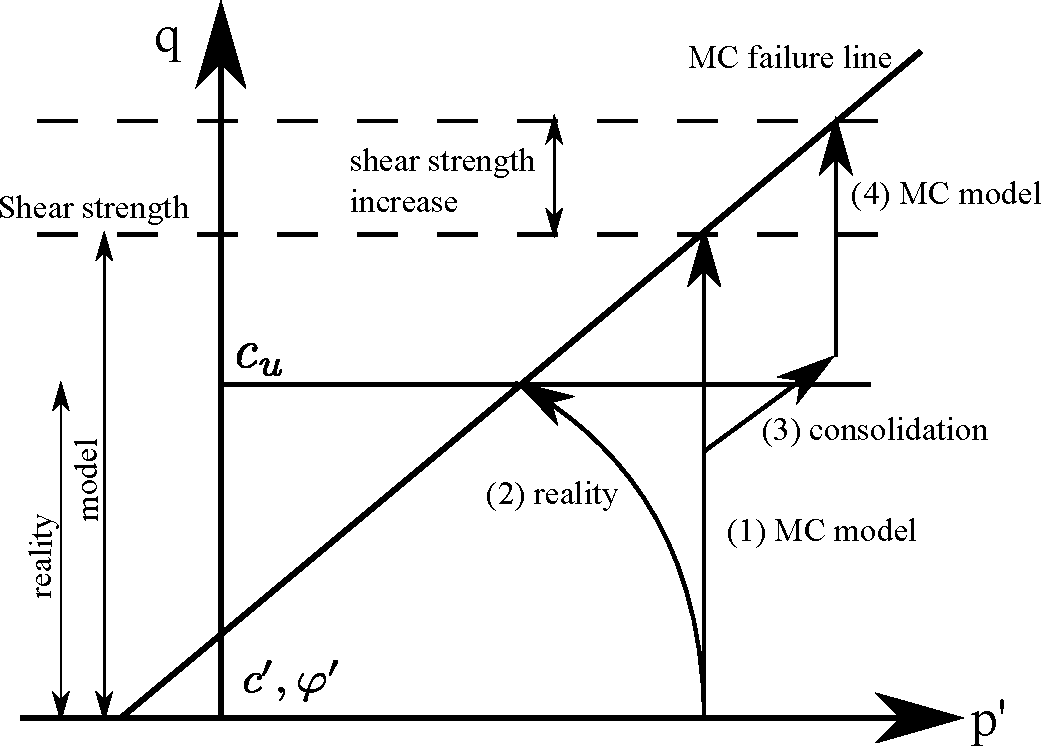
\includegraphics[width=0.75\textwidth]{figs/mc_undrained}
	\end{figure}
}
\mode<handout>{
	\vspace{6cm}
}
\end{frame}

%------------------------------------------------
\begin{frame}
\frametitle{Steps to perform Finite Element Analysis}
\mode<beamer>{
	\begin{enumerate}
	\item \textbf{Define the problem}
	\begin{itemize}
		\item Total stress analysis, effective stress analysis or consolidation
		analysis?
		\item What are the unknowns?
		\item Spatial dimension (plane strain, axisymmetric, 3D)
		\item Element types
	\end{itemize}	
	\item \textbf{Create finite element mesh}
	\item Proper discretization and avoid bad elements
	\item \textbf{Define analysis (or construction sequence) steps}
	\begin{itemize}
		\item apply loading and boundary conditions
	\end{itemize}
	\item \textbf{Define materials}
	\begin{itemize}
		\item determine material properties
	\end{itemize}
	\item \textbf{Assign materials and element types to elements} 
	\item \textbf{Define in-situ stress conditions}
	\item \textbf{Run the analysis}
	\item \textbf{Check! Check! Check!}
	\end{enumerate}
}
\mode<handout>{
	\vspace{6cm}
}
\end{frame}

\section{Slope stability}
%------------------------------------------------
\begin{frame}
\frametitle{2014 Oso landslide}
	\begin{figure}[ht]
		\centering
		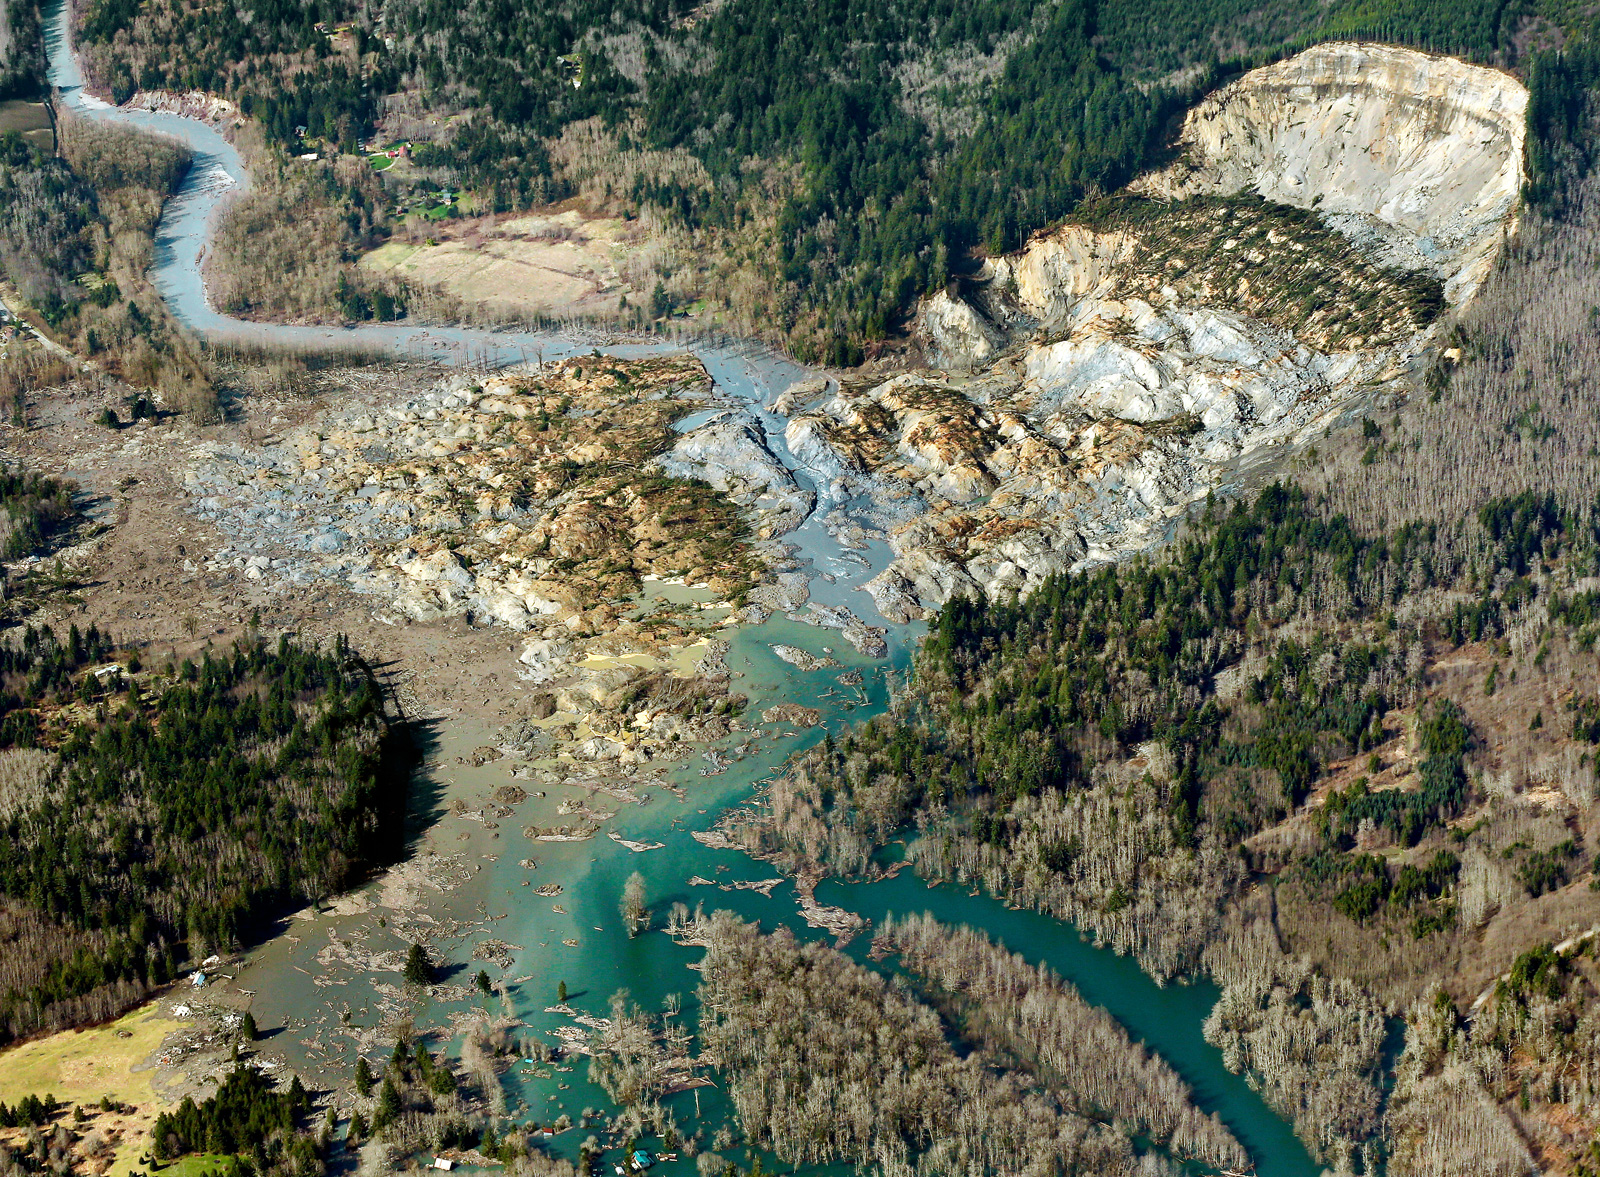
\includegraphics[width=\textwidth]{figs/oso-mudslide.jpg}
	\end{figure}
\end{frame}

\note{
	\begin{itemize}
		\item 22nd March 2014 at 10.37 am
		\item Volume: approx. 8 million m3
		\item 43 casualties (deadliest landslide in US)
		\item 1 neighboured destroyed
		\item \textbf{Cost unknown} but $>$ USD 150 million + USD 65 million (lawsuit 2017) + indirect costs
		\item Social tensions (general public \& sc. community)
		\item Indian Snohomish tribe
	\end{itemize}
}

%------------------------------------------------
\begin{frame}
\frametitle{Shear failure plane}
\begin{figure}[ht]
	\centering
	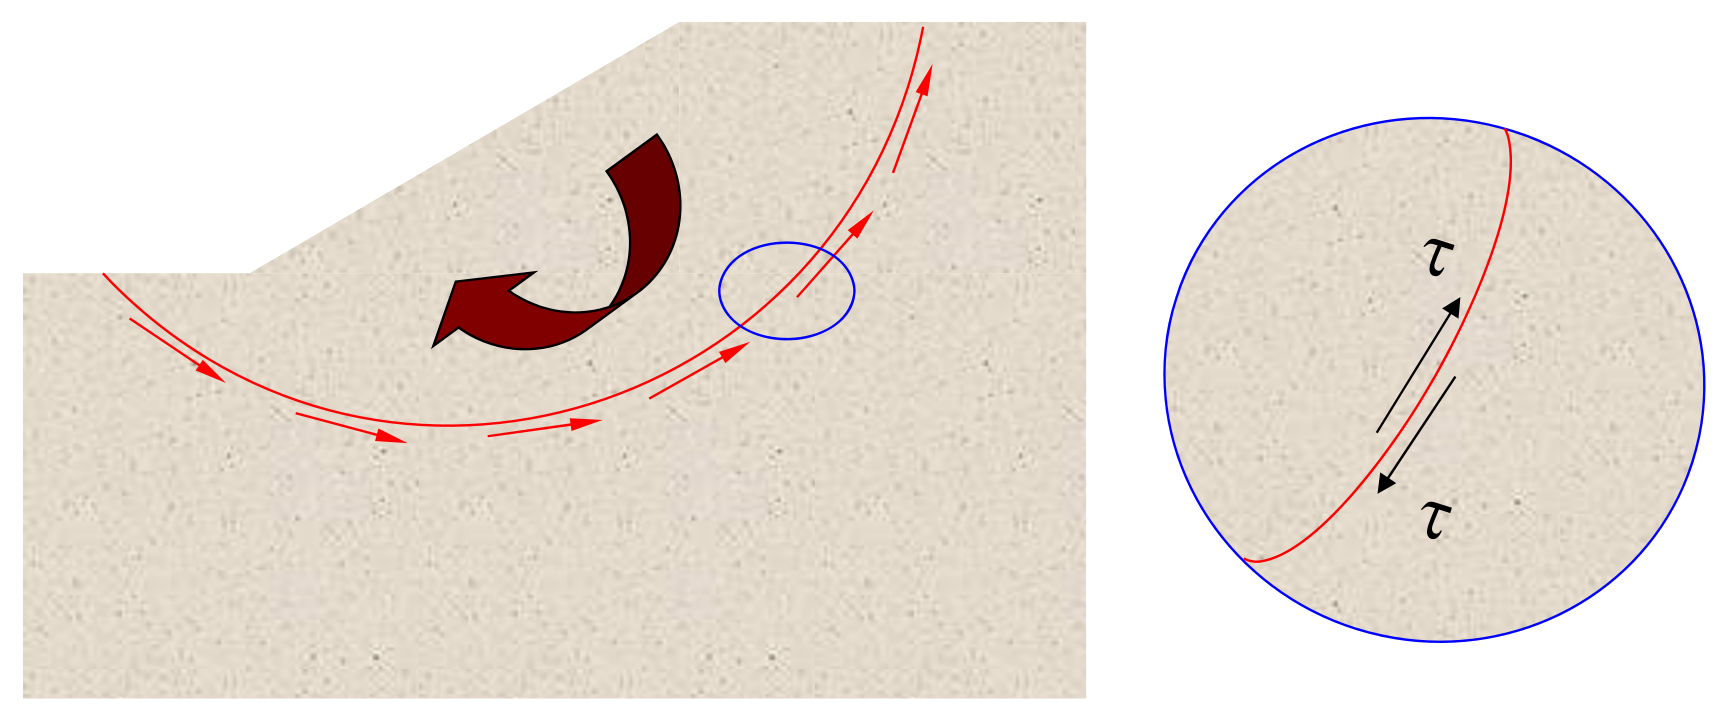
\includegraphics[width=0.9\textwidth]{figs/shear-failure-plane.png}
	\caption*{At failure, shear stress along the failure surface ($\tau$) reaches the shear strength ($\tau_f$).}
\end{figure}
Factor of Safety = \mode<beamer>{Resistance (from soil shear strength)/Driving force (from total
stress equilibrium (i.e. weight of the soil))}
\end{frame}

%------------------------------------------------
\begin{frame}
\frametitle{Dry slope (total stress = effective stress)}
\mode<beamer>{
	\begin{figure}[ht]
		\centering
		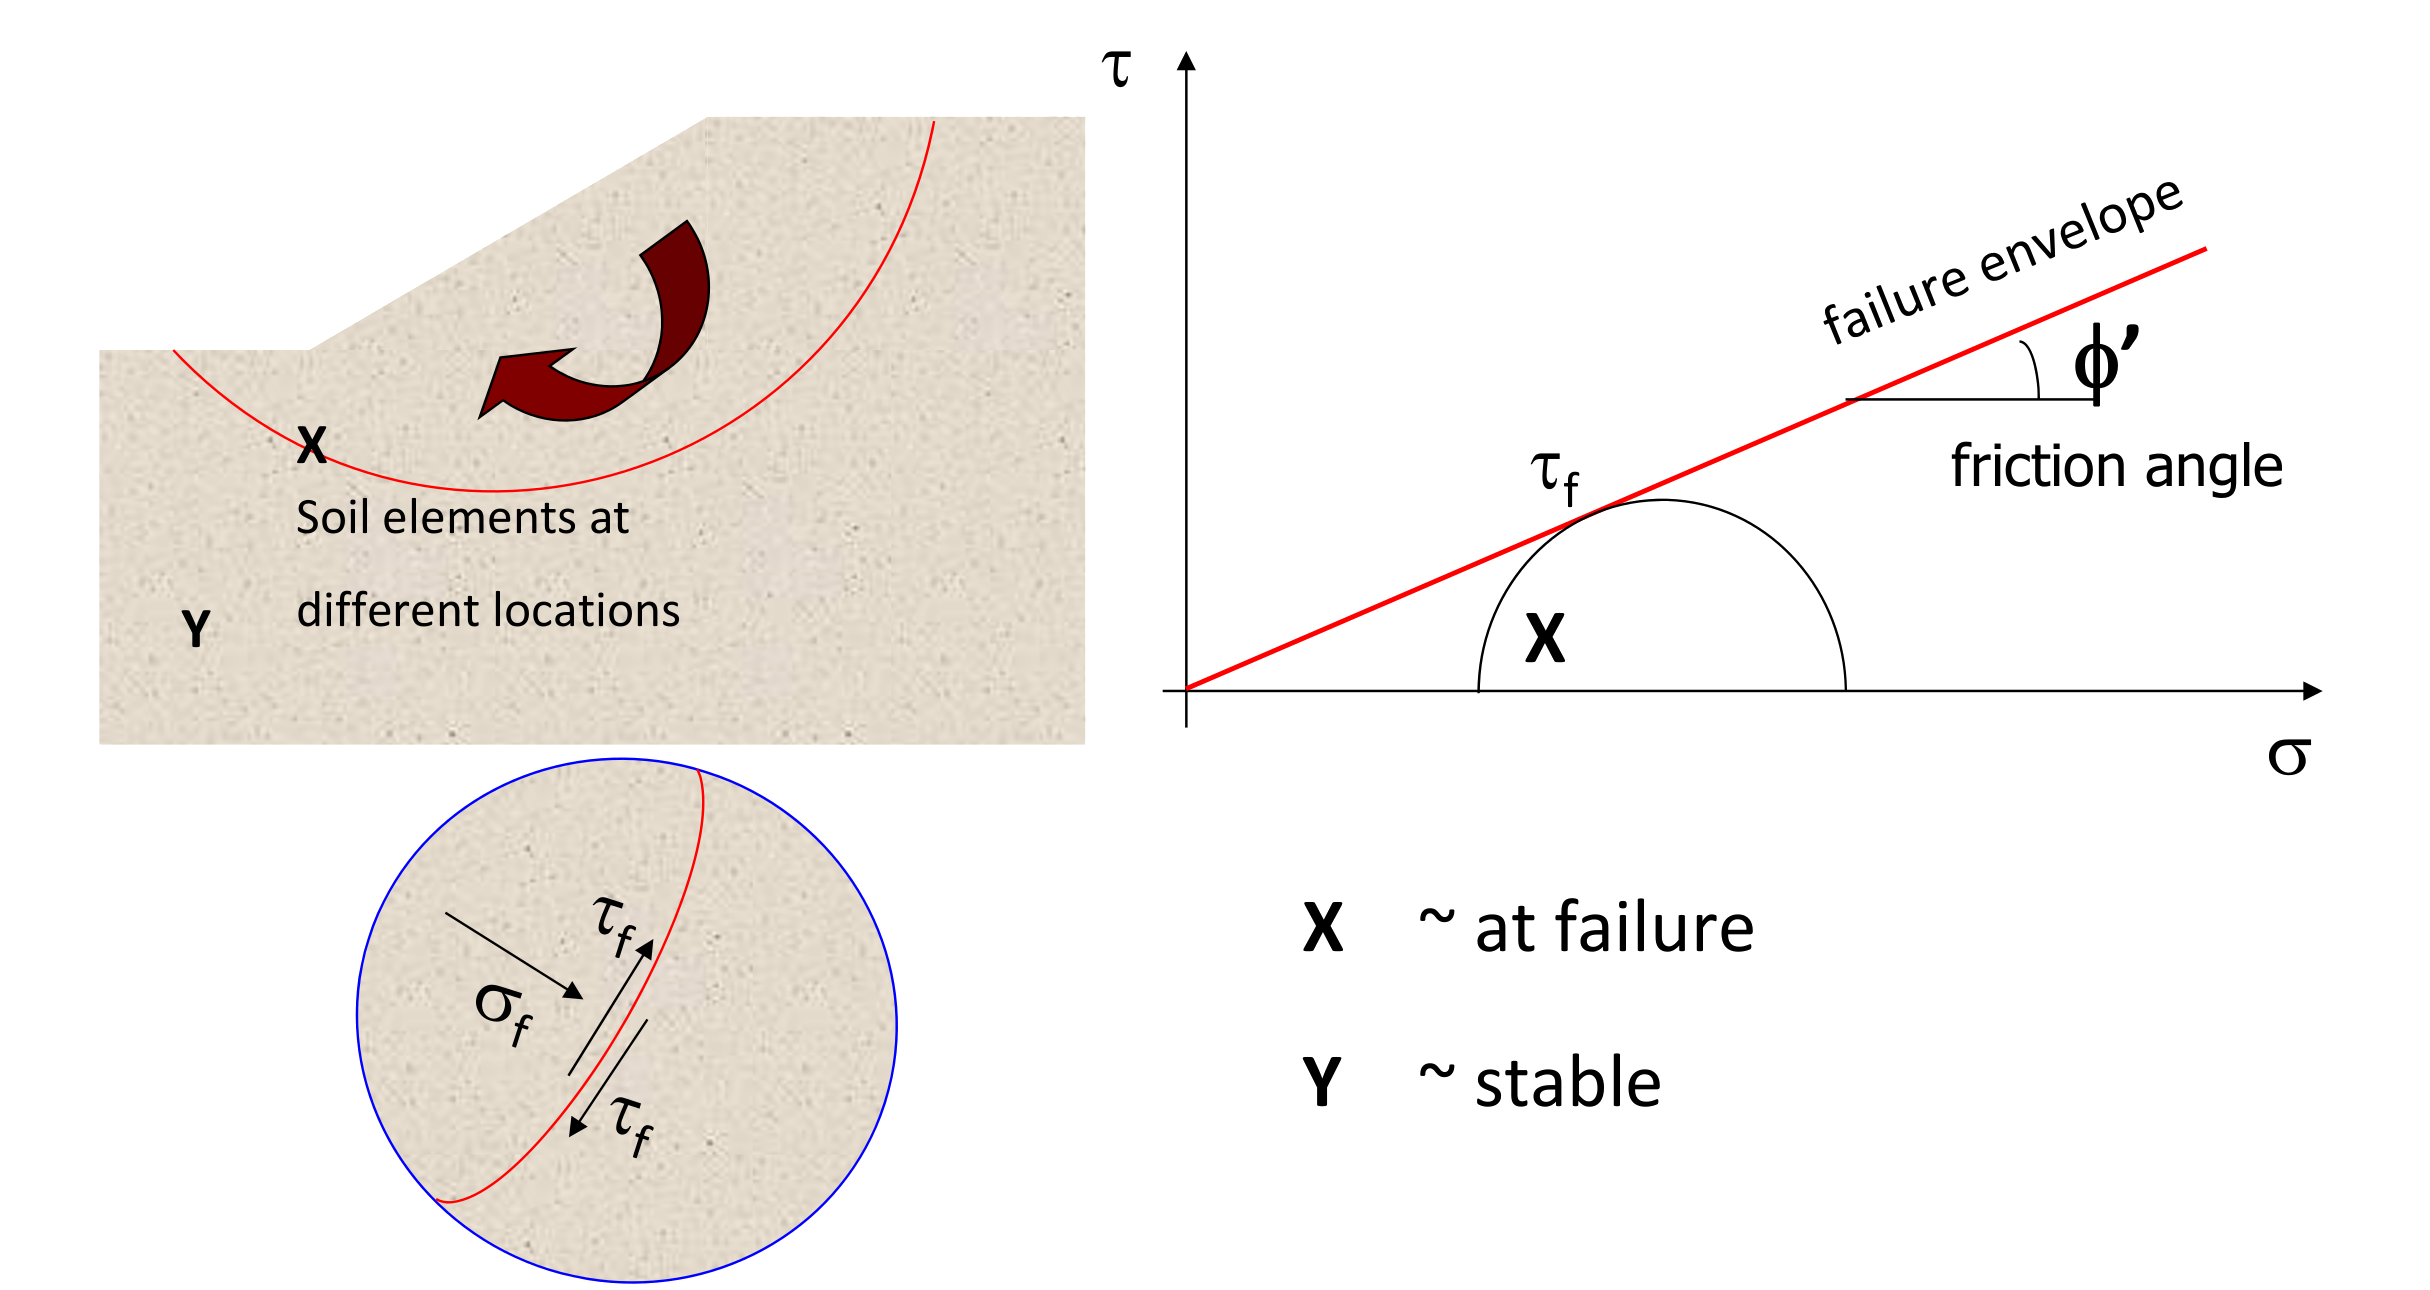
\includegraphics[width=\textwidth]{figs/dry-slope.png}
	\end{figure}
}
\mode<handout>{
	\begin{figure}[ht]
		\centering
		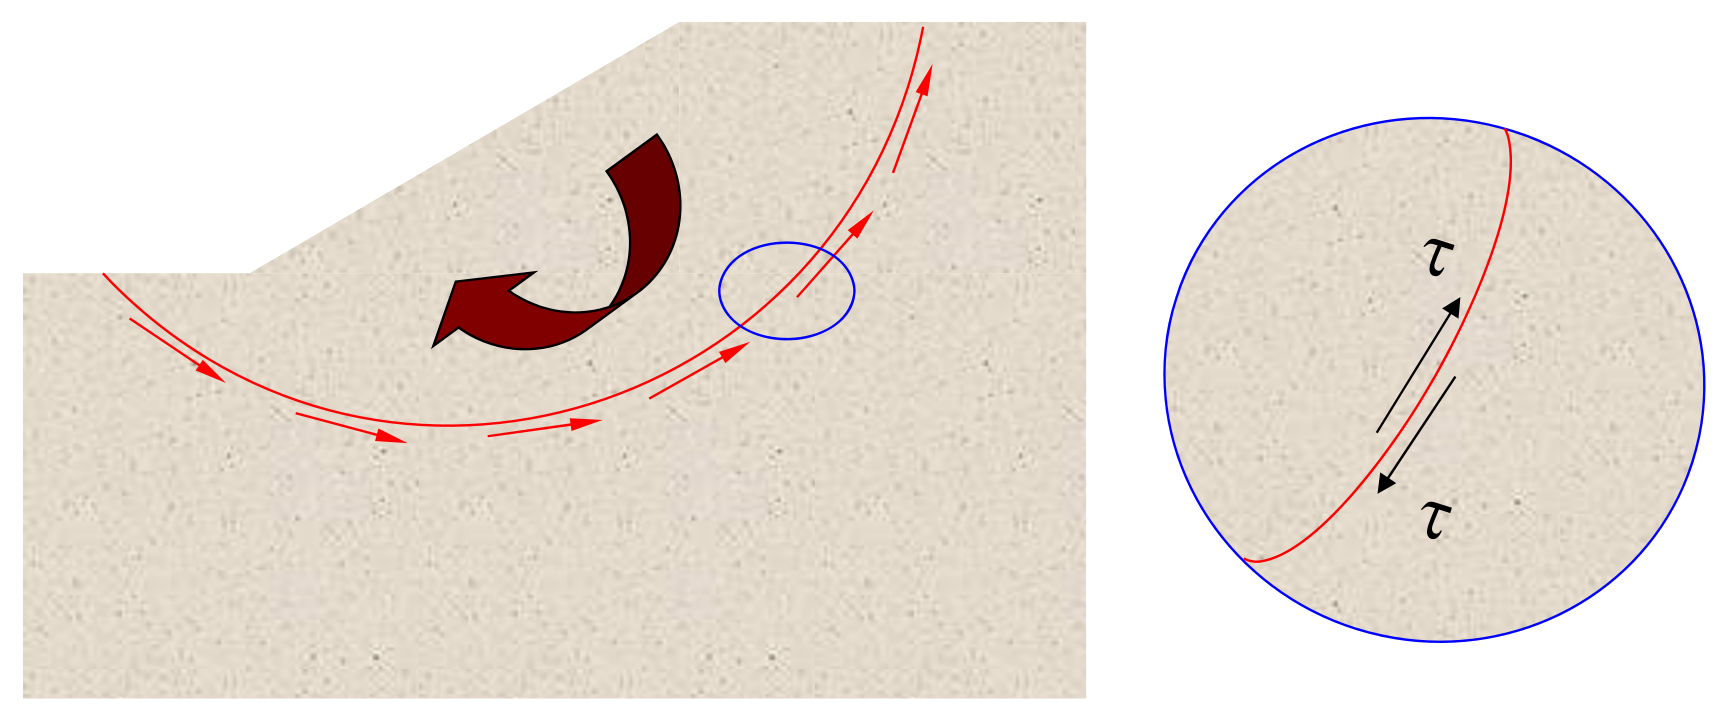
\includegraphics[width=0.9\textwidth]{figs/shear-failure-plane.png}
	\end{figure}
}
\end{frame}

%------------------------------------------------
\begin{frame}
\frametitle{Saturated slope (total stress = effective stress + pwp)}
\textbf{Drained conditions} - need to compute the steady state pore pressure field
and then evaluate ``effective stress‐based'' shear strength to find the overall
stability (based on total stress equilibrium).
\mode<beamer>{
	\begin{figure}[ht]
		\centering
		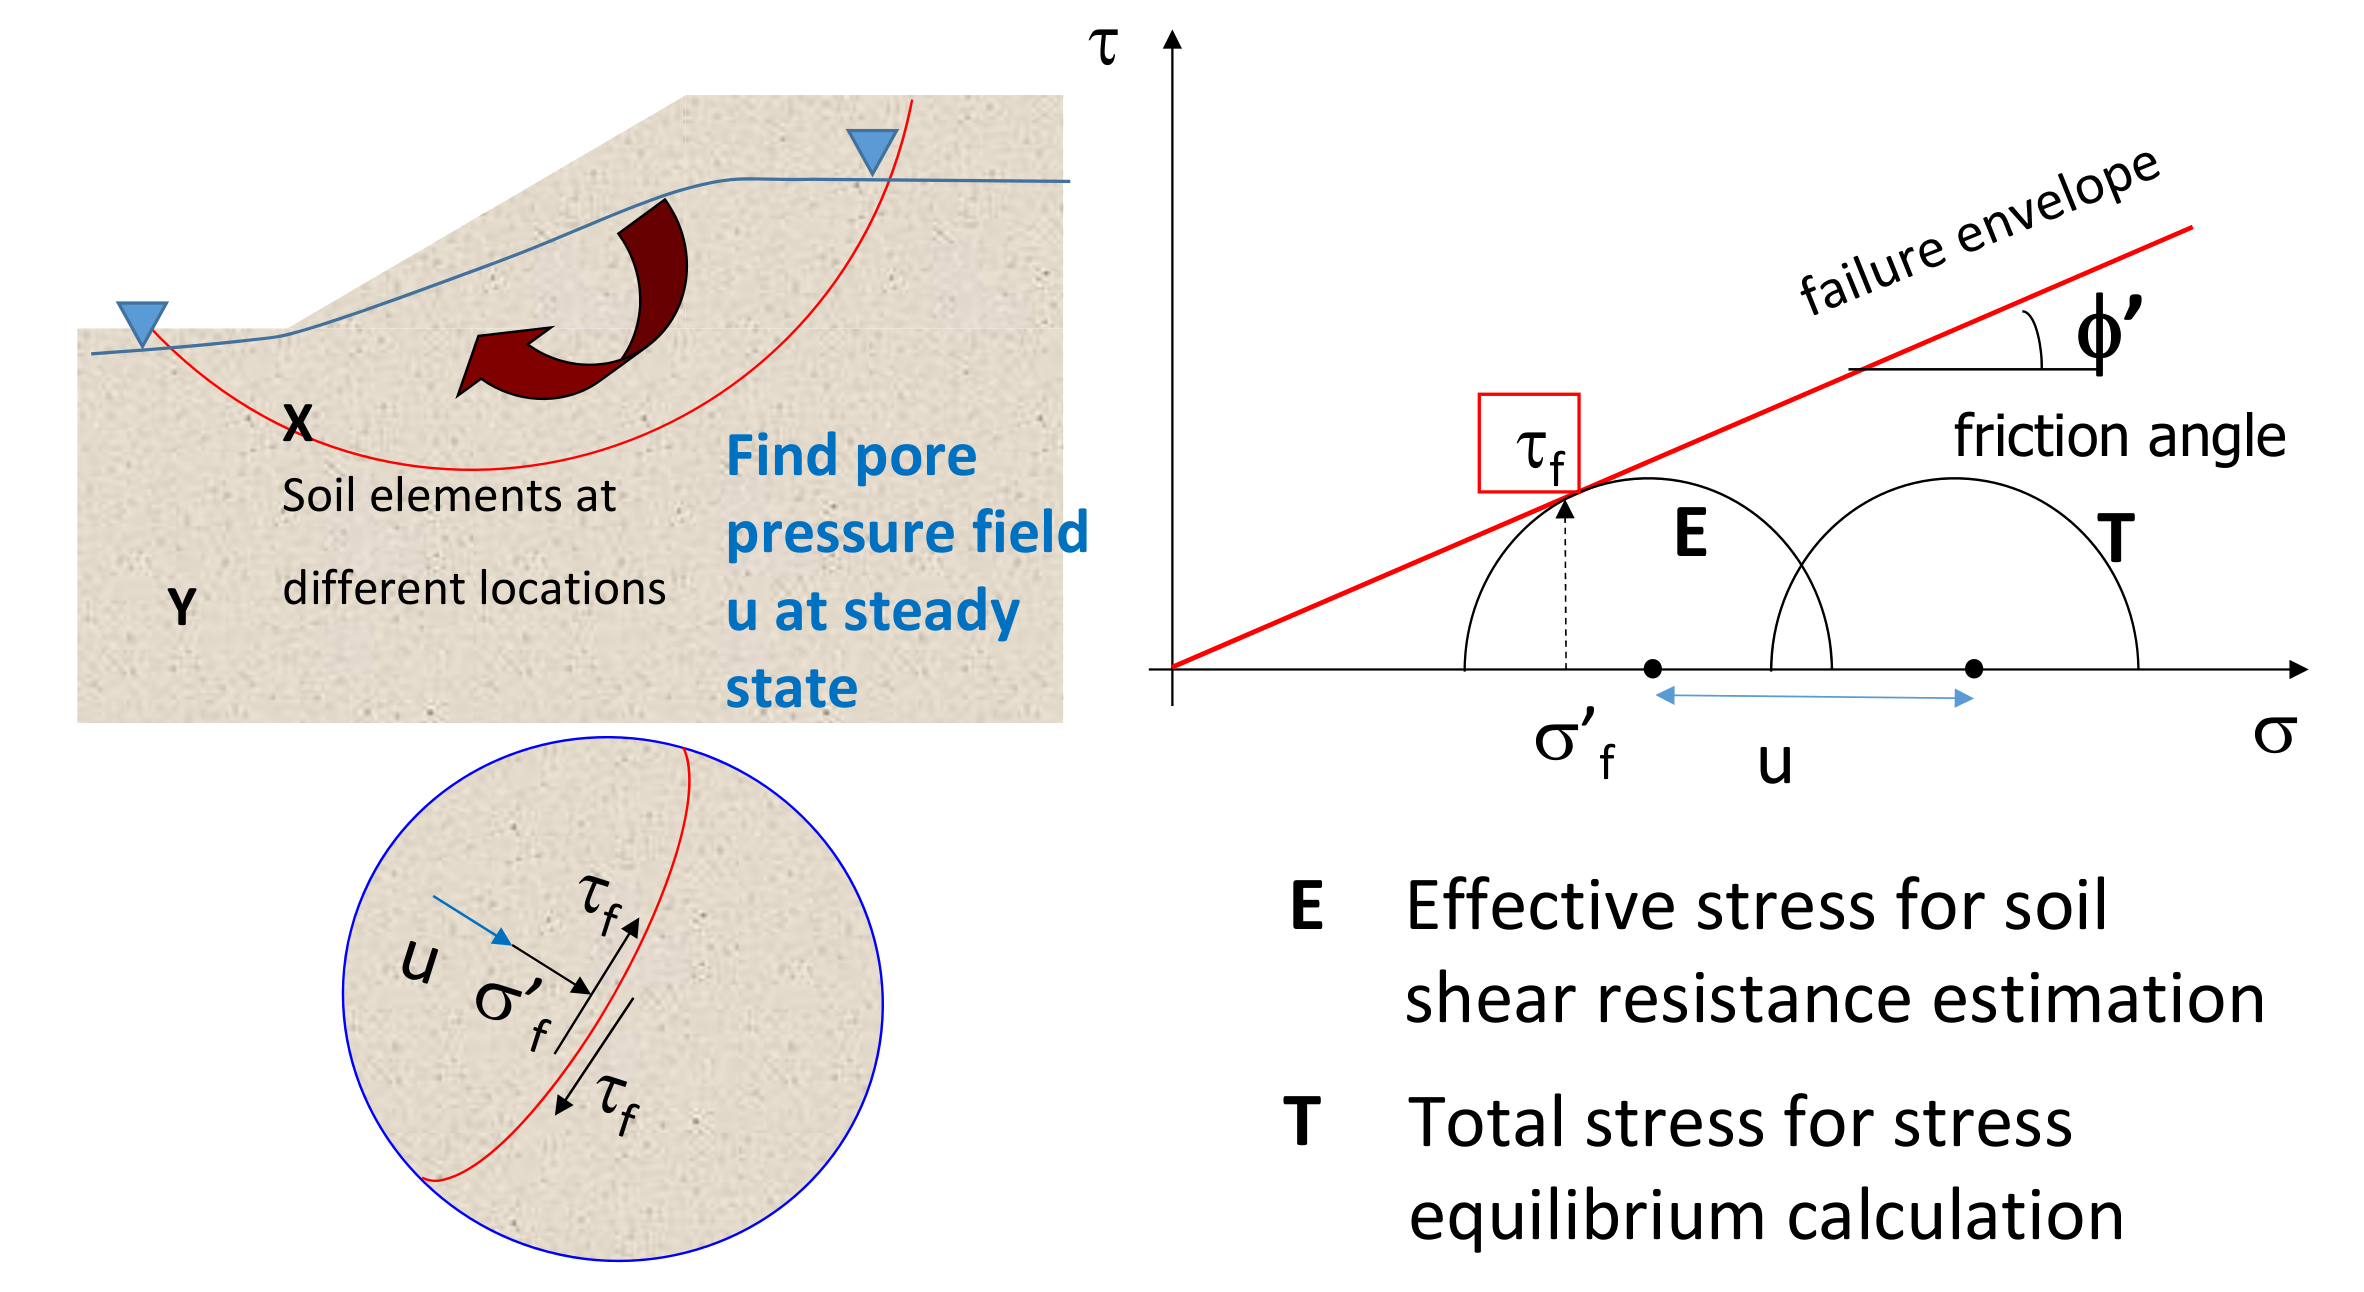
\includegraphics[width=\textwidth]{figs/saturated-slope.png}
	\end{figure}
}
\mode<handout>{
	\begin{figure}[ht]
		\centering
		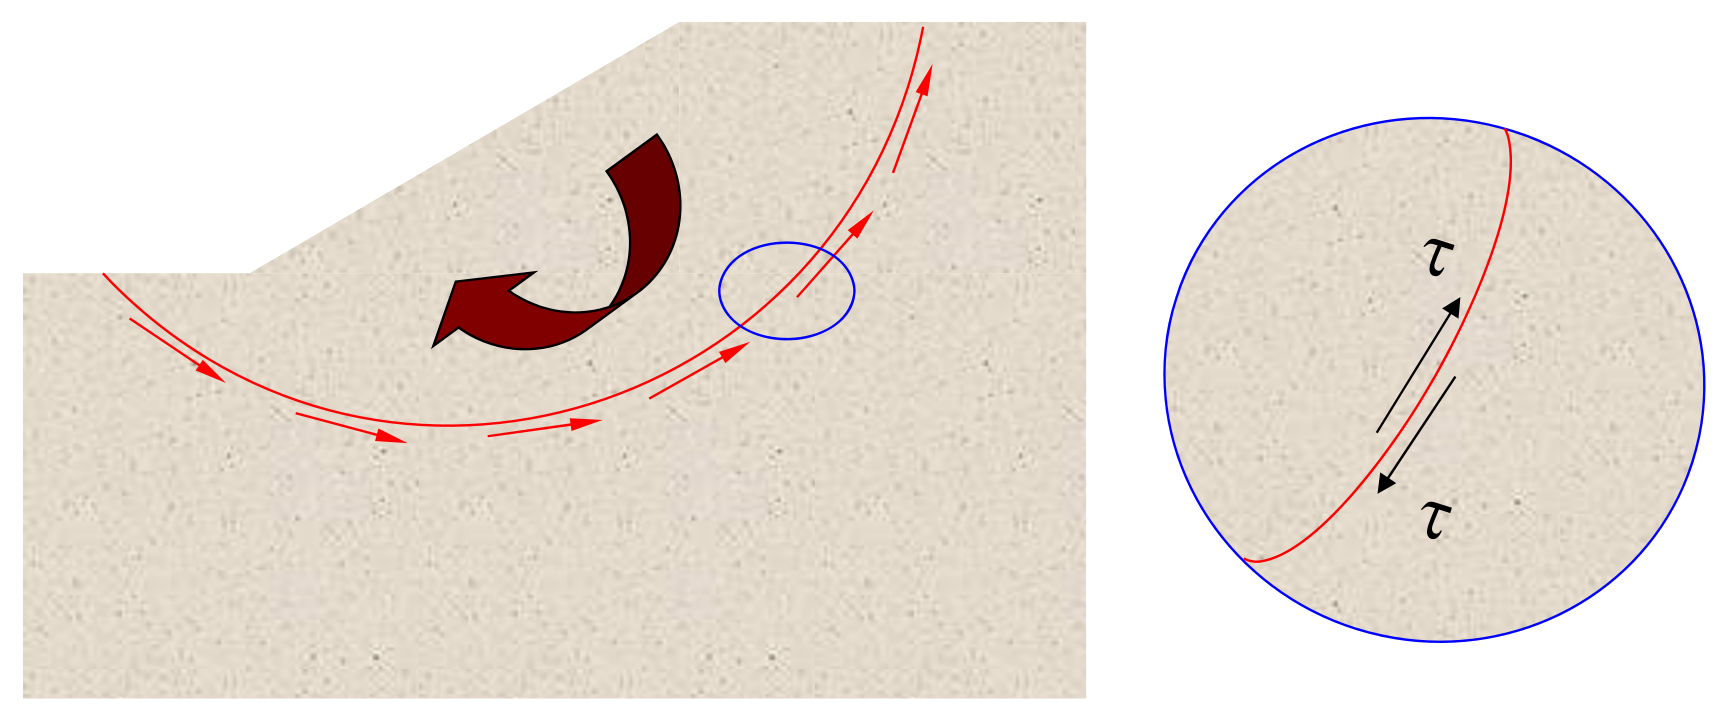
\includegraphics[width=0.9\textwidth]{figs/shear-failure-plane.png}
	\end{figure}
}
\end{frame}

%------------------------------------------------
\begin{frame}
\frametitle{Saturated slope (total stress = effective stress + PWP)}
\textbf{Undrained conditions} ‐ (total stress approach) – Use ``\textit{total‐stress based}''
shear strength ($s_u$) to find the overall stability (based on total stress
equilibrium).
\mode<beamer>{
	\begin{figure}[ht]
		\centering
		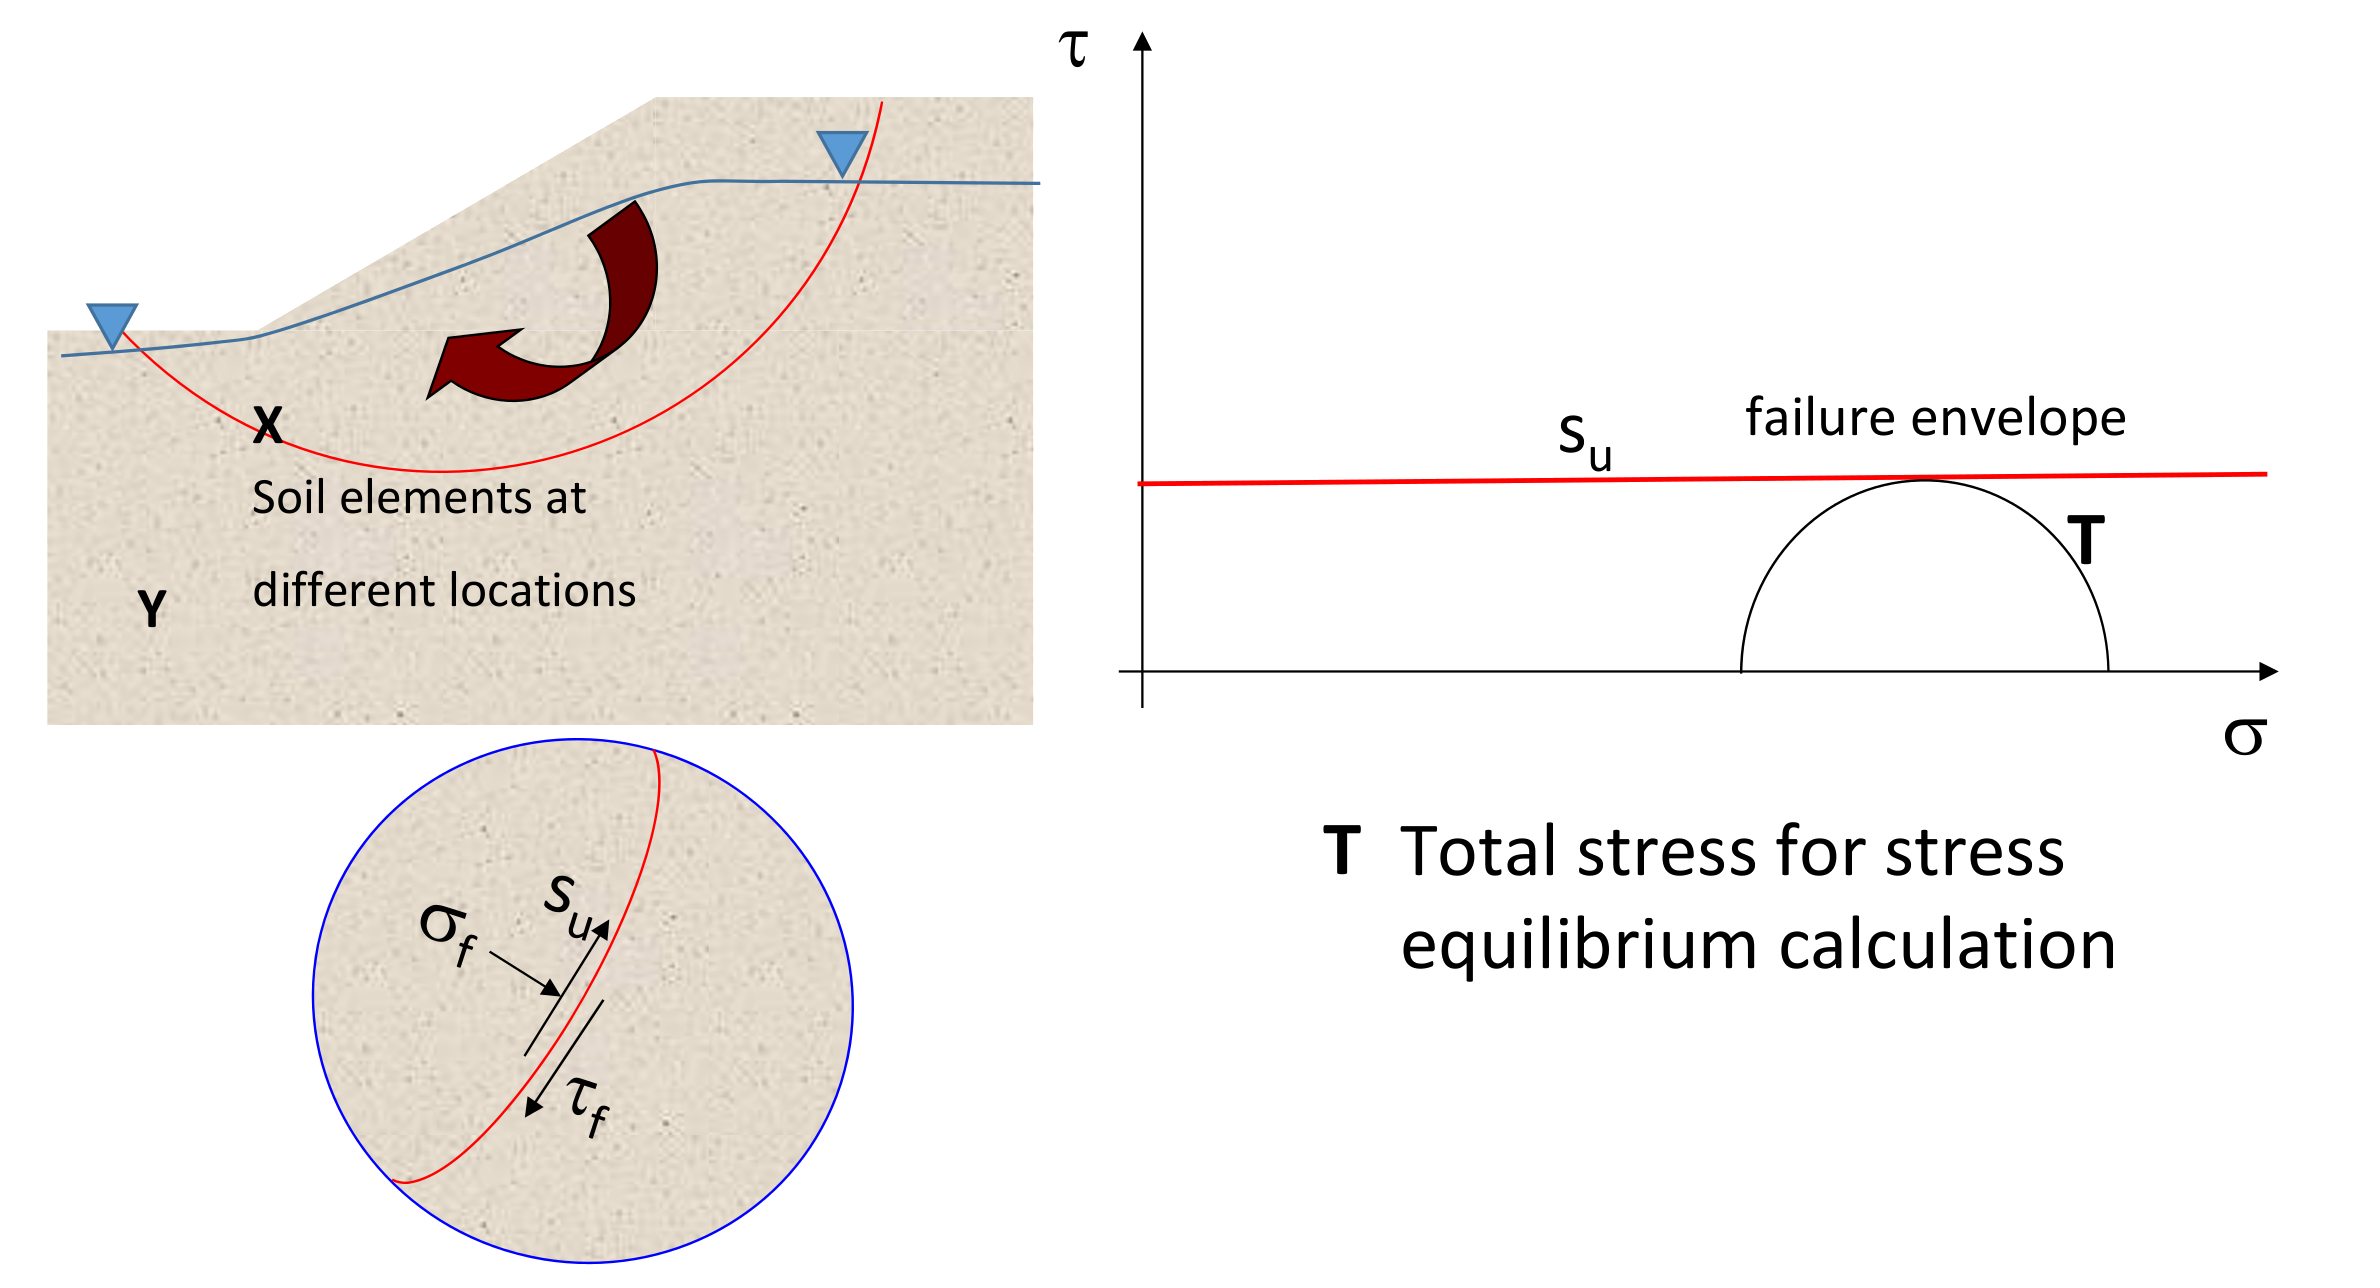
\includegraphics[width=\textwidth]{figs/saturated-undrained.png}
	\end{figure}
}
\mode<handout>{
	\begin{figure}[ht]
		\centering
		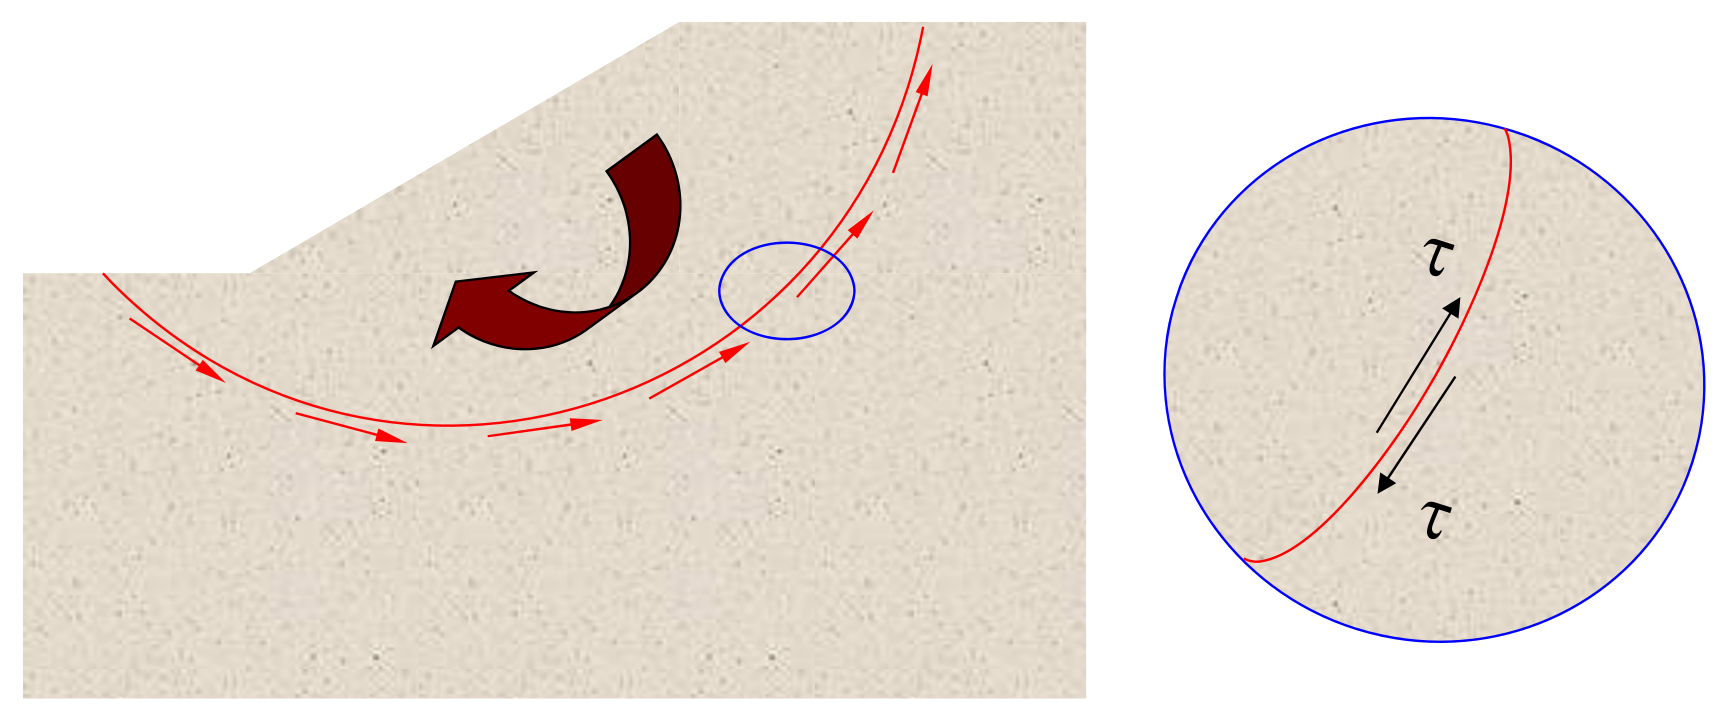
\includegraphics[width=0.9\textwidth]{figs/shear-failure-plane.png}
	\end{figure}
}
\end{frame}

%------------------------------------------------
\begin{frame}
\frametitle{Saturated slope (total stress = effective stress + PWP)}
\textbf{Undrained conditions} ‐ (Effective stress approach‐not common) ‐ need to
compute the pore pressure (including excess pore pressure) field and then
evaluate ``\textit{effective stress ‐based}'' shear strength to find the overall stability
(based on total stress equilibrium).
\mode<beamer>{
	\begin{figure}[ht]
		\centering
		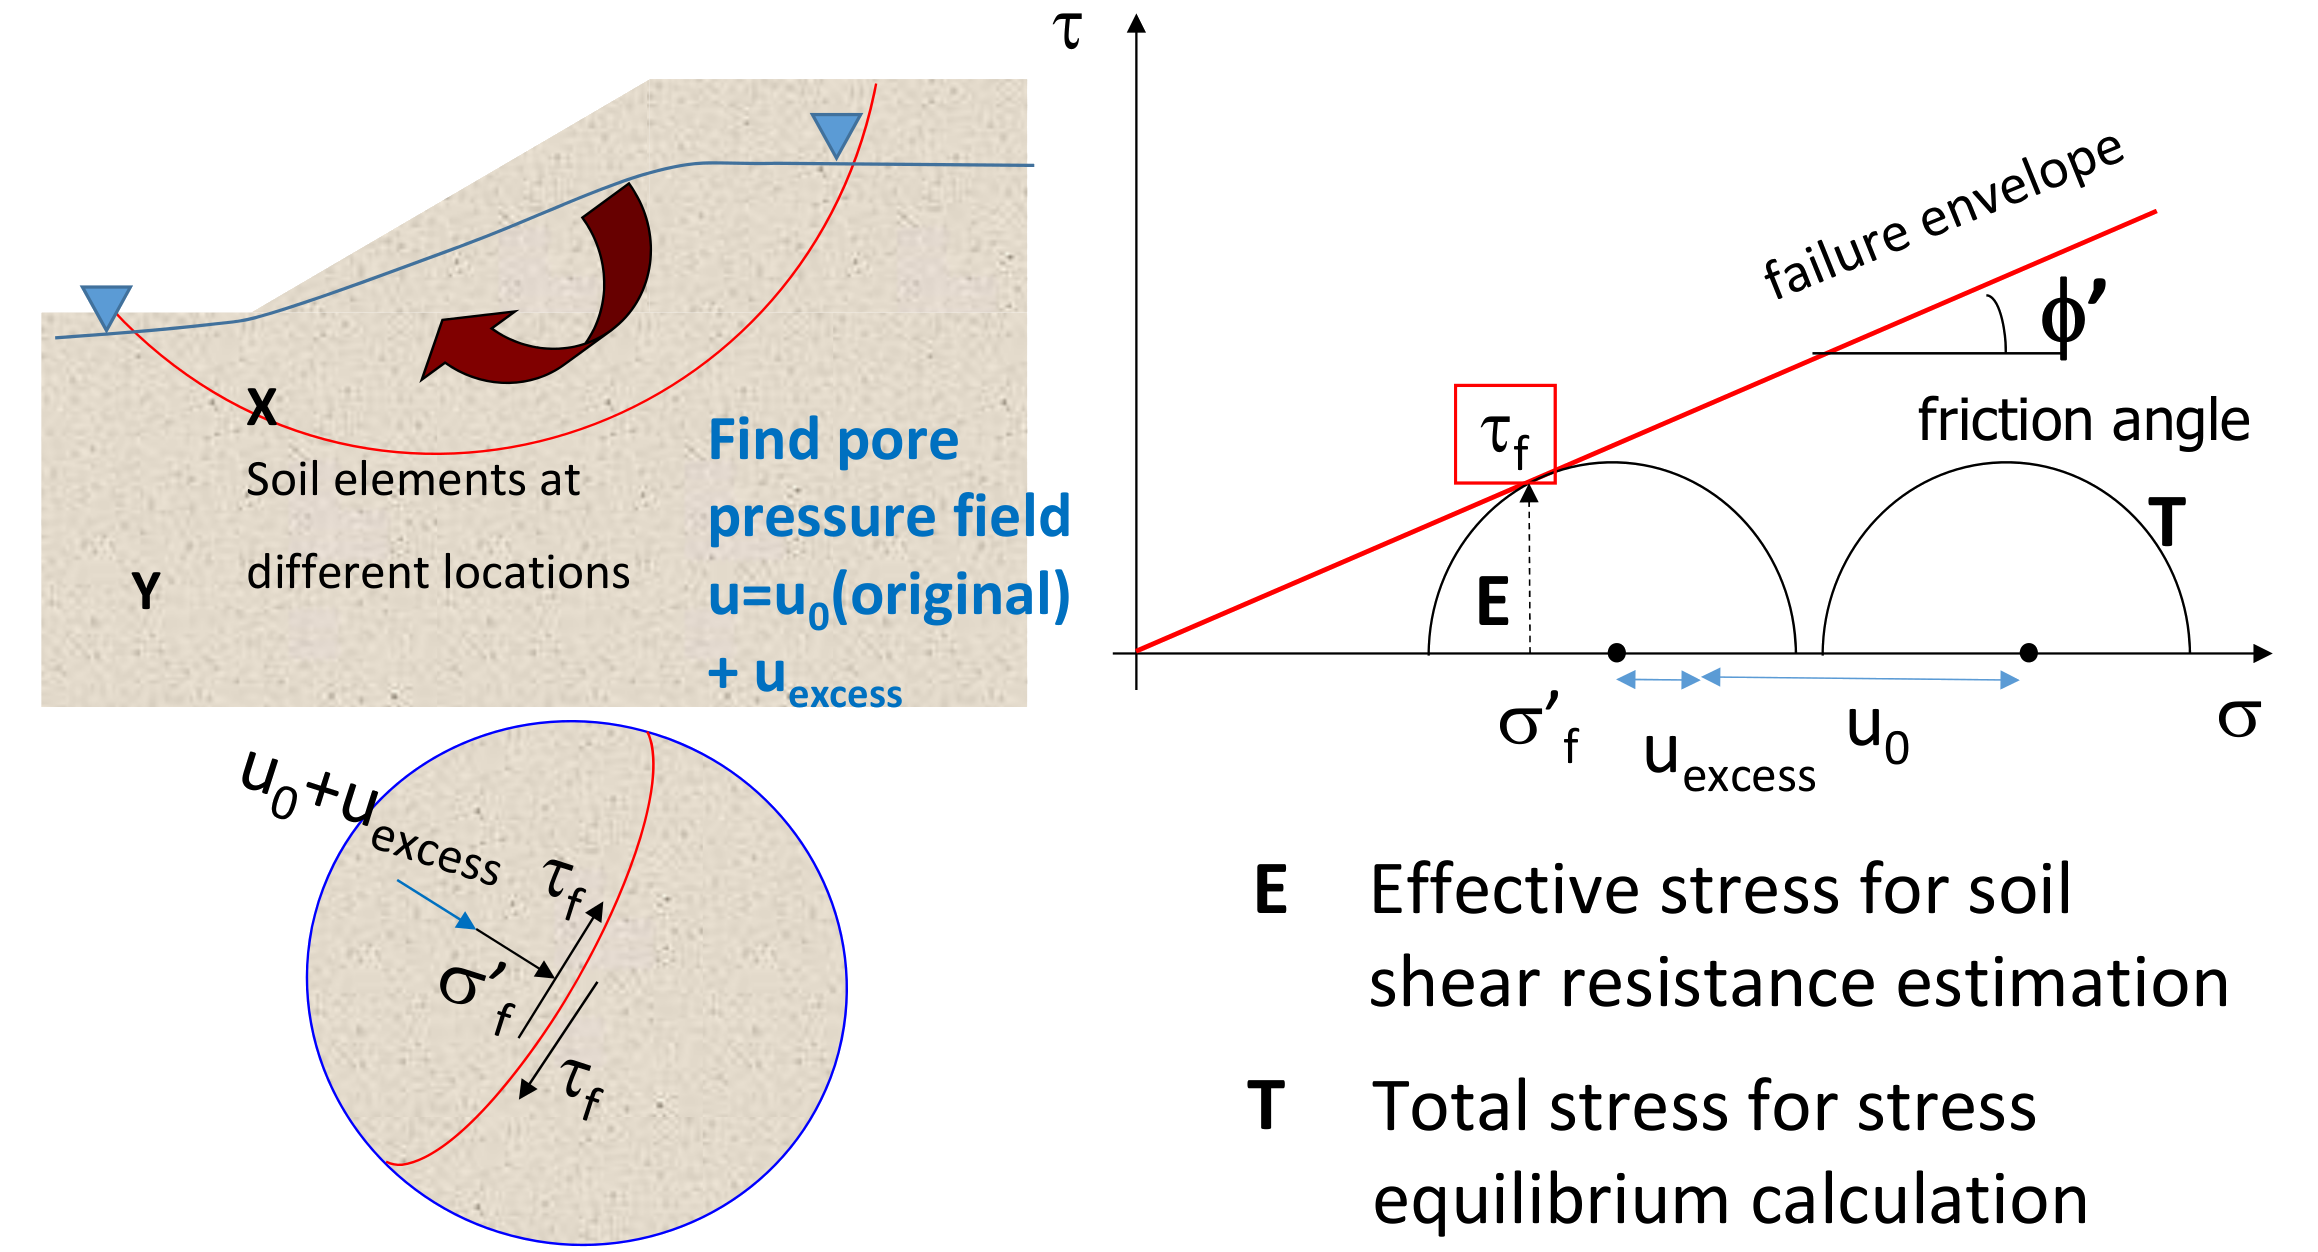
\includegraphics[width=\textwidth]{figs/undrained-effective-stress.png}
	\end{figure}
}
\mode<handout>{
	\begin{figure}[ht]
		\centering
		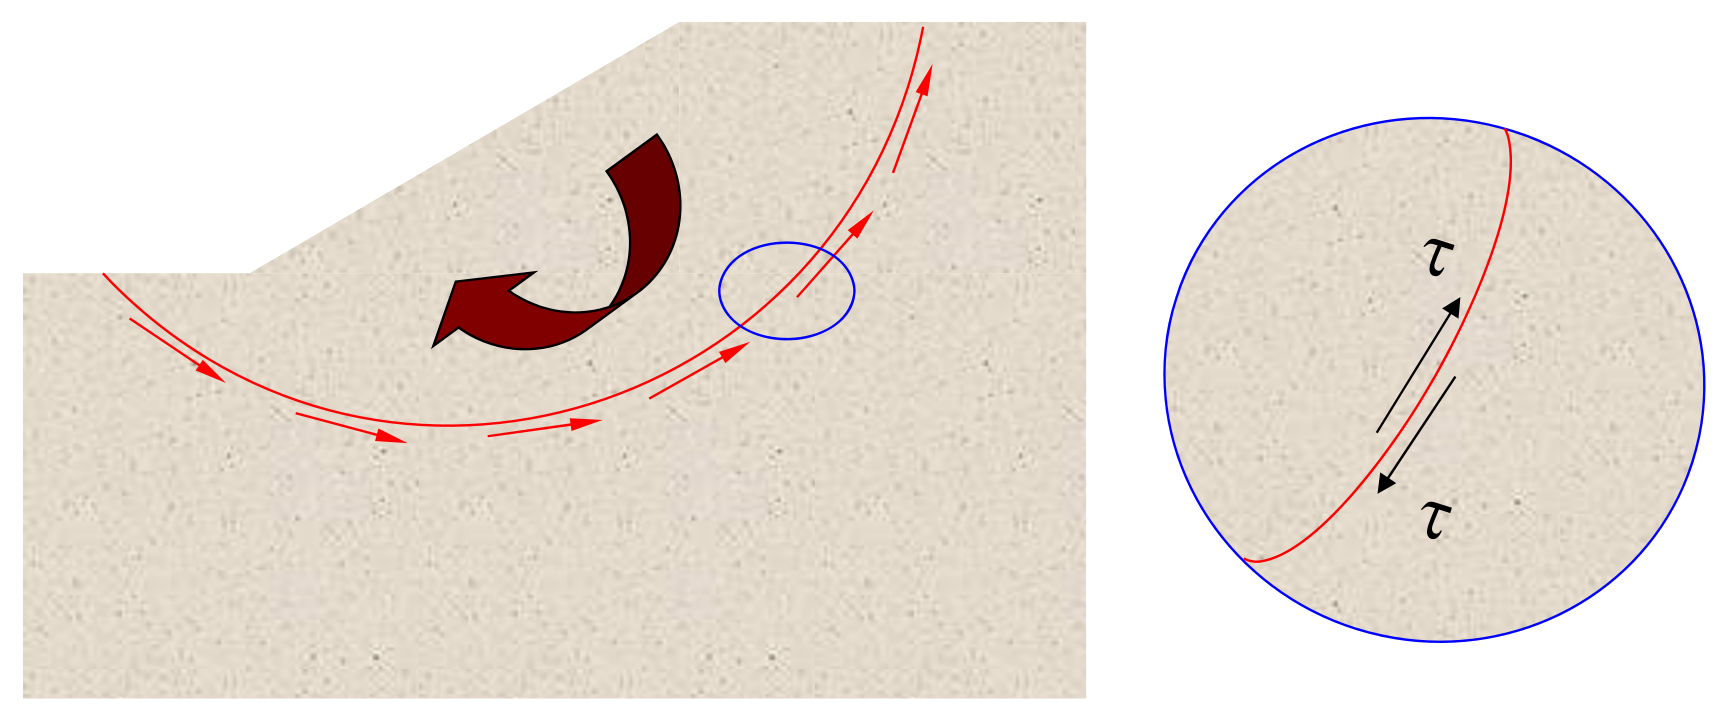
\includegraphics[width=0.9\textwidth]{figs/shear-failure-plane.png}
	\end{figure}
}
\end{frame}

%------------------------------------------------
\begin{frame}
\frametitle{Infinite slopes}
\begin{figure}[ht]
	\centering
	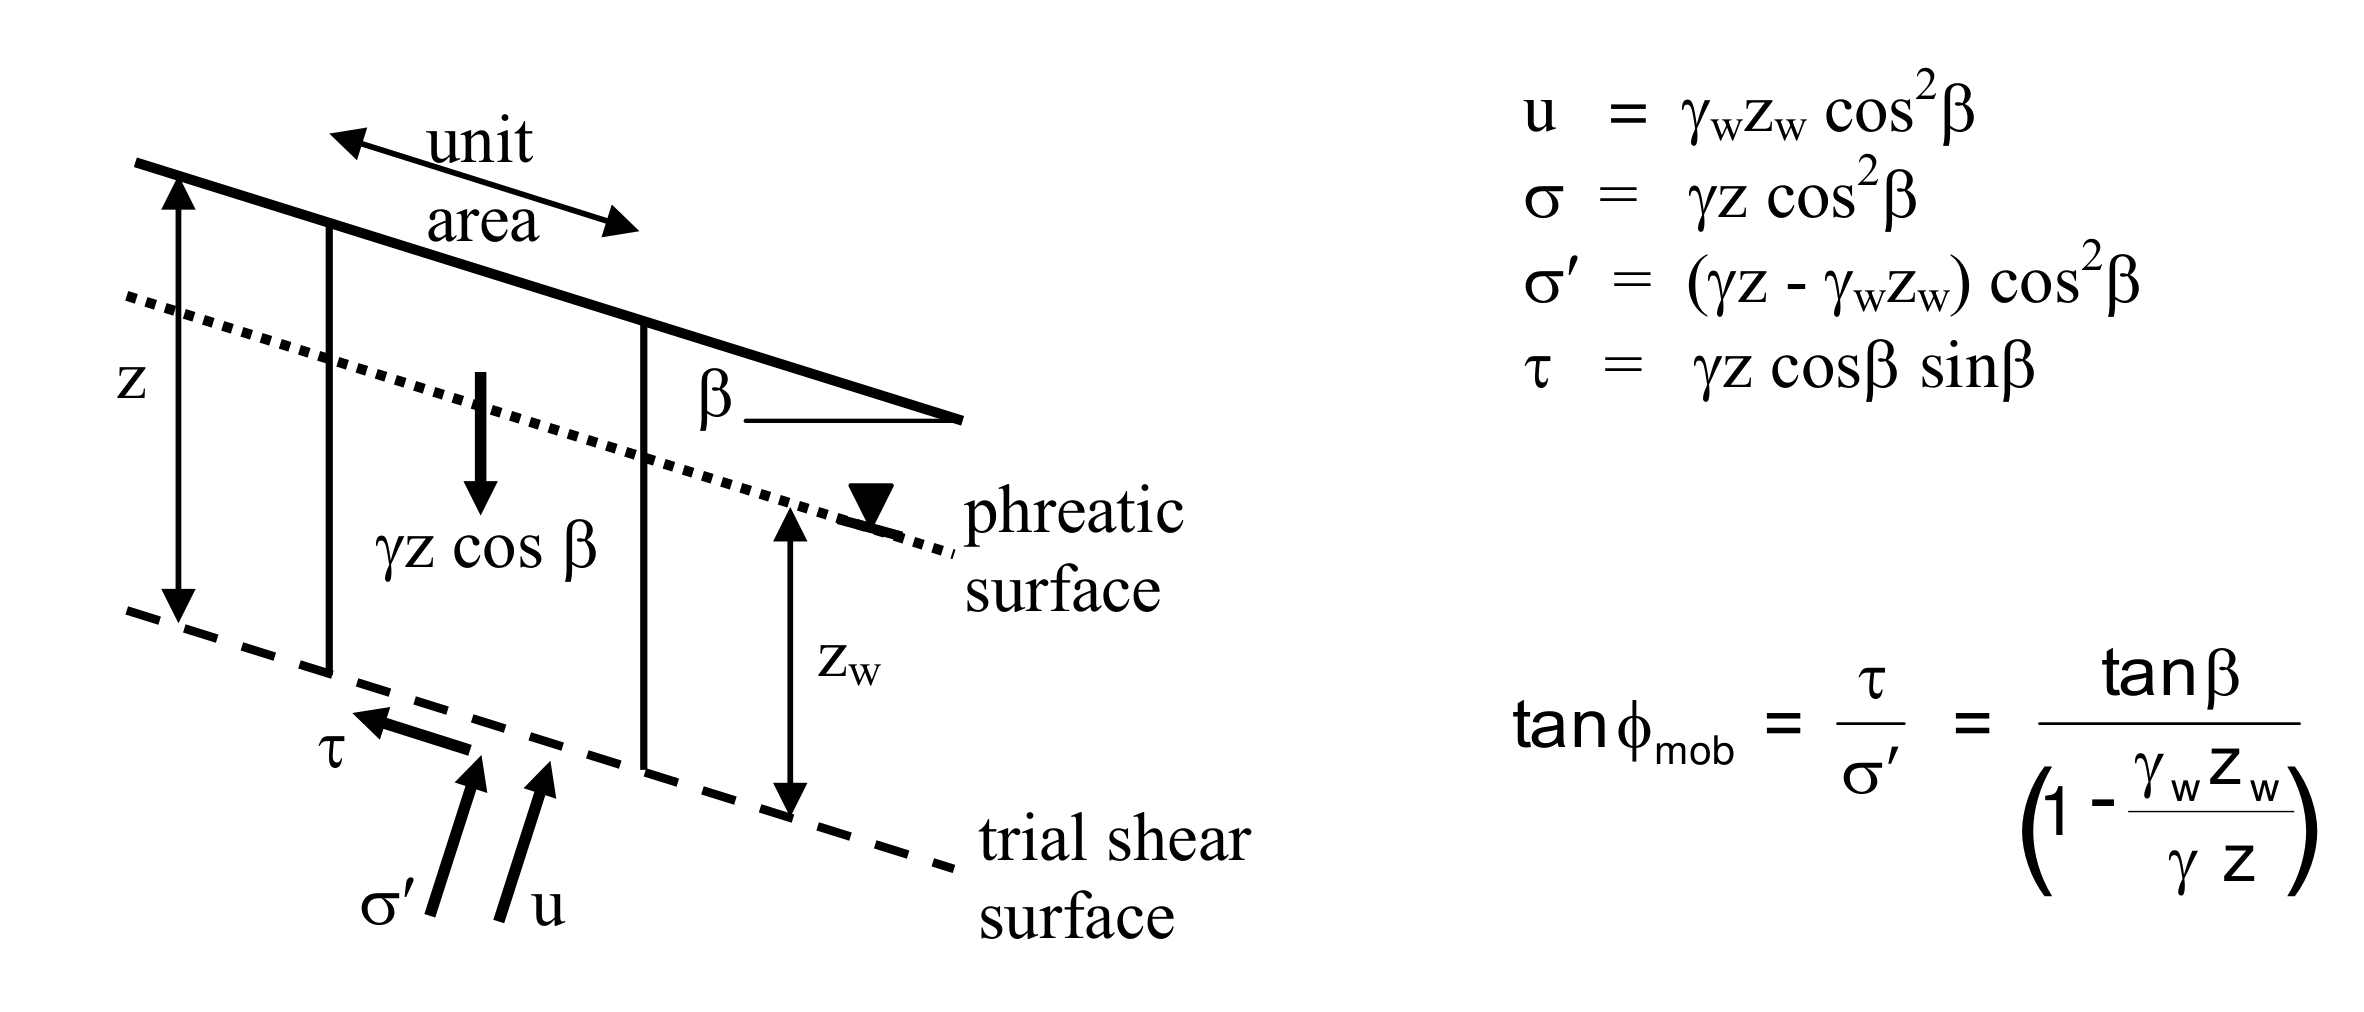
\includegraphics[width=0.9\textwidth]{figs/infinite-slope.png}
\end{figure}
Soil fails when (dry): \mode<beamer>{$ \beta = \phi_{\mathrm{mob}}$}
Soil fails when (submerged): \mode<beamer>{$ \beta = \phi_{\mathrm{mob}}$}
\end{frame}

\note{
	Slope with steady state seepage (drained): $\tan(\beta) = (1 – \gamma_w /\gamma) \tan(\phi_{\mathrm{mob}})$

}

%------------------------------------------------
\begin{frame}
\frametitle{Undrained infinite slope (total stress approach)}
\begin{figure}[ht]
	\centering
	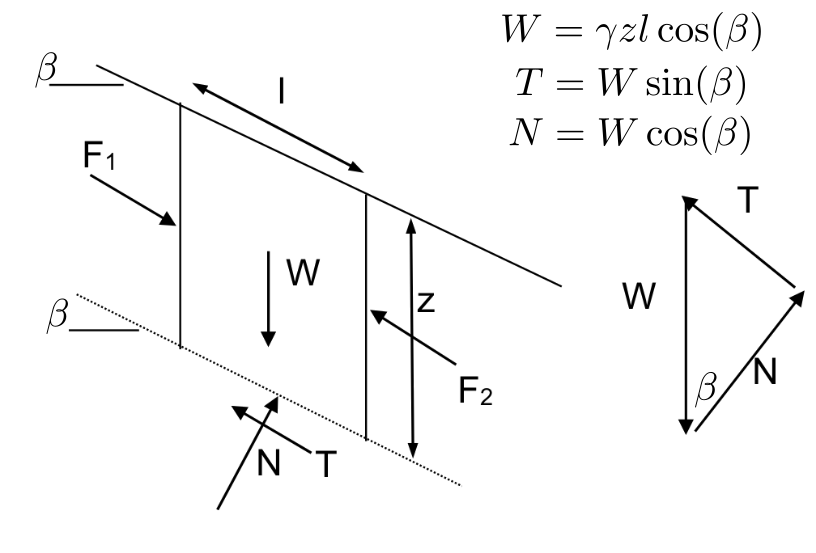
\includegraphics[width=0.85\textwidth]{figs/undrained-infinite-slope.png}
\end{figure}
But also the shear stress: \mode<beamer>{$ T =  s_u l$. The slope failure is governed by $s_u$ profile (with depth).}
\end{frame}


%------------------------------------------------
\begin{frame}
\frametitle{Infinite slope: Summary}
\begin{figure}[ht]
	\centering
	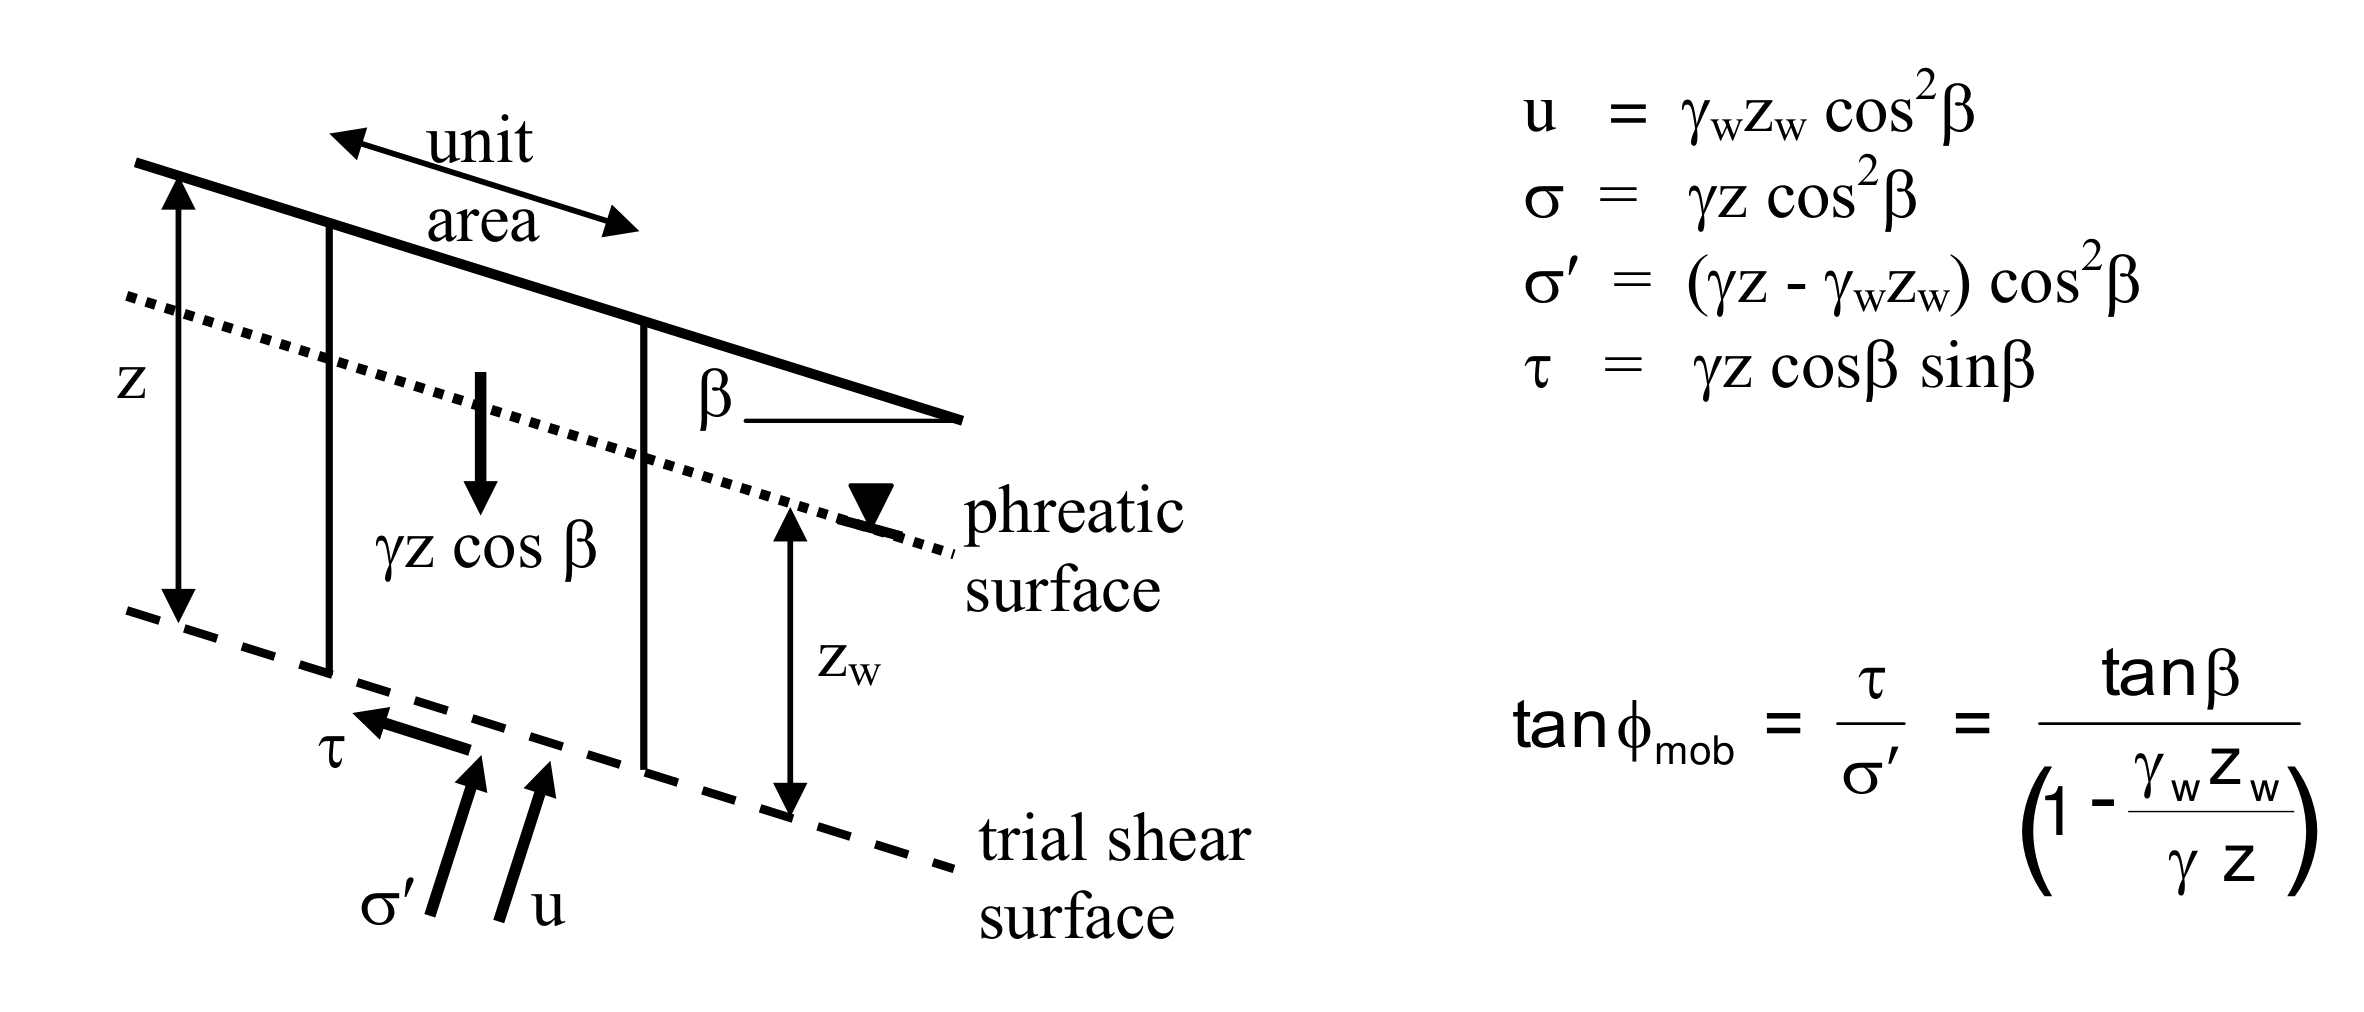
\includegraphics[width=0.6\textwidth]{figs/infinite-slope.png}
\end{figure}
\begin{enumerate}
	\item Factor of Safety = resistance / driving
	\item Dry FoS = $\tan(\phi_{\mathrm{mob}})/\tan(\beta)$
	\item Submerged FoS = $\tan(\phi_{\mathrm{mob}})/\tan(\beta)$
	\item Undrained FoS = $2 s_u / \gamma z \sin(2 \beta)$
	\item Steady state seepage FoS = $(1 - \gamma_w/ \gamma) \tan(\phi_{\mathrm{mob}})/\tan(\beta)$ where the water table is located at the slope surface
\end{enumerate}
\end{frame}

\end{document}